%%%%%%%%%%%%%%%%%%%%%%%%%%%%%%%%%%%%%%%%%%%%%%%%%%%%%%%%%%%%%%%%%%%%%%%%%%%%
%
%  ludwig.tex
%
%  Long-hand documentation for Ludwig. This file is main document
%  with style only. Content is in sections.tex
%
%  Edinburgh Soft Matter and Statistical Physics Group and
%  Edinburgh Parallel Computing Centre
%
%  Kevin Stratford (kevin@epcc.ed.ac.uk)
%  (c) 2008-2014 The University of Edinburgh
%
%%%%%%%%%%%%%%%%%%%%%%%%%%%%%%%%%%%%%%%%%%%%%%%%%%%%%%%%%%%%%%%%%%%%%%%%%%%%

\documentclass[11pt,twoside]{article}

\usepackage{amsmath}
\usepackage{moreverb}
\usepackage{lscape}
\usepackage{epic}
\usepackage[pdftex]{graphicx}
\usepackage{bm}
\usepackage{hyperref}
\usepackage{color}
\usepackage{listings}
\usepackage{mathtools}

\setlength{\hoffset}{-1in}
\setlength{\voffset}{-1in}

\setlength{\topmargin}{2cm}
\setlength{\evensidemargin}{3.1cm}
\setlength{\oddsidemargin}{3.1cm}

\setlength{\textwidth}{14.8cm}
\setlength{\textheight}{23cm}

\setlength{\parindent}{0pt}
\setlength{\parskip}{\smallskipamount}




\newcommand{\inputkey}[1]{\framebox{\textbf{\texttt{#1}}}}
\newcommand{\e}[1]{\cdot10^{#1}}
\newcommand{\beq}{\begin{equation}}
\newcommand{\eeq}{\end{equation}}
\newcommand{\beqa}{\begin{eqnarray}}
\newcommand{\eeqa}{\end{eqnarray}}
\newcommand{\com}[1]{\textcolor{red}{#1}}
\newcommand{\cur}[1]{{\textit{#1}}}

\definecolor{terminalcolour}{gray}{0.96}

\lstdefinestyle{terminalverbatim}{
  basicstyle=\small\ttfamily,
  columns=flexible,
  backgroundcolor=\color{terminalcolour},
  xleftmargin=0pt
}


\begin{document}


\setcounter{page}{1}

%\tableofcontents

\newpage
\lstset{style=terminalverbatim}

\setcounter{page}{1}

% These redefinitions are just compressing the spacing a little.

\makeatletter
\renewcommand*{\section}{%
\@startsection {section}{1}{\z@}%
  {-1.75ex \@plus -0.5ex \@minus -.1ex}%
  {1.15ex \@plus.1ex}%
  {\normalfont\Large\bfseries}%
}
\renewcommand*{\subsection}{%
\@startsection {subsection}{2}{\z@}%
  {-1.75ex \@plus -0.5ex \@minus -.1ex}%
  {1.15ex \@plus.1ex}%
  {\normalfont\large\bfseries}%
}
\renewcommand*{\subsubsection}{%
\@startsection {subsubsection}{1}{\z@}%
  {-1.75ex \@plus -0.5ex \@minus -.1ex}%
  {1.15ex \@plus.1ex}%
  {\normalfont\normalsize\bfseries}%
}

% Sections

%%%%%%%%%%%%%%%%%%%%%%%%%%%%%%%%%%%%%%%%%%%%%%%%%%%%%%%%%%%%%%%%%%%%%%%%%%%%%%
%
%  intro.tex
%
%  Contains introduction and quick start for users.
%
%  Edinburgh Soft Matter and Statistical Physics Group and
%  Edinburgh Parallel Computing Centre
%
%  (c) 2016-2018 The University of Edinburgh
%
%%%%%%%%%%%%%%%%%%%%%%%%%%%%%%%%%%%%%%%%%%%%%%%%%%%%%%%%%%%%%%%%%%%%%%%%%%%%%%

\section{Introduction}

\subsection{Overview}

This introduction provides a brief overview of what the \textit{Ludwig} code
does, how to obtain and build it, and how to run a sample problem.
It is assumed that the reader has at least a general knowledge
of Navier-Stokes hydrodynamics, complex fluids, and to some
extent statistical physics. This knowledge will be required to make sense
of the input and output involved in using the code. Those wanting
to work on or develop the code itself will need knowledge of ANSI C,
and perhaps message passing and CUDA. We assume the reader is using
a Unix-based system.

\subsubsection{Purpose of the code}

The \textit{Ludwig} code has been developed over a number of
years to address specific problems in complex fluids. The underlying
hydrodynamic model is based on the lattice Boltzmann equation
(LBE, or just `LB'). This itself may be used to study simple
(Newtonian) fluids in a number of different scenarios, including porous
media and particle suspensions. However, the
code is more generally suited to complex fluids, where a number of
options are available, among others: symmetric binary fluids and
Brazovskii smectics,
polar gels, liquid crystals, or charged fluid via a Poisson-Boltzmann
equation approach. These features are added in the framework of a
free energy approach, where specific compositional or orientational
order parameters are evolved according to the appropriate
coarse-grained dynamics, but also interact with the fluid in a
fully coupled fashion.

A number of other features are catered for is some or all situations.
These include fluctuating hydrodynamics, and appropriate fluctuating
versions of order parameter dynamics for binary solvents and liquid
crystals. Colloidal particles are available for simulation of
suspensions and dispersions, and with appropriate boundary
conditions binary mixtures, liquid crystals, and charged fluid. Shear
flow is available for fluid-only systems implemented via Lees-Edwards
sliding periodic boundaries. Not all these features play with all the
others: check the specific section of the document for details.

Broadly, the code is intended for complex fluid problems at low
Reynolds numbers, so there is no consideration of turbulence,
high Mach number flows, high density ratio flows, and so on.

\subsubsection{How the code works}

We aim to provide a robust and portable code, written in ANSI C, which
can be used to perform serial and scalable parallel simulations of
complex fluid systems based around hydrodynamics via the lattice
Boltzmann method. Time evolution of modelled quantities takes
place on a fixed regular discrete lattice. The preferred method of
dealing with the corresponding order parameter equations is by
using finite difference. However, for the case of a binary fluid,
a two-distribution lattice Boltzmann approach is also maintained
for historical reference.

Users control the operation of the code via a plain text input file;
output for various data are available. These data may be visualised
using appropriate third-party software (e.g., Paraview). Specific
diagnostic output may require alterations to the code.

Potential users should also note that the complex fluid simulations
enabled by \textit{Ludwig} can be time consuming, prone to instability,
and provide results which are difficult to
interpret. We make no apology for this: that's the way it is.

\subsubsection{Who should read what?}

This documentation is aimed largely at users, but includes information
that will also be relevant for developers. The documentation discusses
the underlying features of the coordinate system, hydrodynamics (LB), and
other generic features, and has a separate section for each free energy.
You will need to consult the section relevant to your problem.


\subsection{Obtaining the code}

The code is publicly available from
\texttt{http://github/ludwig-cf/ludwig/}
which provides revision control via git, issue tracking, and so on.

The current stable release is available as the master branch.


\vfill
\pagebreak

\section{Quick Start for Users}

This section provides a brief overview of compiling and running
the code, which should allow users to get off the ground.
The section assumes the code has been downloaded and you are in the
top level directory.

\subsection{Configuration}

You will need to copy one of the existing configuration files from
the \texttt{config} directory to the top level directory. This file
sets all the relevant local details for compilation and so on. For
example:
\begin{lstlisting}
$ cp config/lunix-gcc-default.mk config.mk
\end{lstlisting}
Edit the new \texttt{config.mk} file to check, or adjust, the options
as required. You will need to identify your local C compiler. The
example uses \texttt{gcc}
in serial, and \texttt{mpicc} in parallel. For MPI in particular,
local details may vary. A quick way to compile the code is via
\begin{lstlisting}
$ cd tests
$ make compile-mpi-d3q19
\end{lstlisting}
This integrates a number of separate stages which are described
indivually in the following sections. The resulting executable
will be \texttt{./src/Ludwig.exe} at the top level.

\subsubsection{targetDP}

A \texttt{targetDP} layer is required by the code in all cases. It
allows compilation for both simple CPU systems and
for a number of accelerator systems using a single source code. This
will make the appropriate choices depending what has been specified
in the top-level \texttt{config.mk} file. From the top-level directory
\begin{lstlisting}
$ cd targetDP
$ make
\end{lstlisting}
should produce the appropriate \texttt{libtarget.a} library.

\subsubsection{Serial}
\label{section:quick-serial}

First, compile the MPI stub library in the \texttt{mpi\_s}
directory. You should be able to build the library and run the
tests using, e.g.:

\begin{lstlisting}
$ make libc
gcc -Wall -I.  -c mpi_serial.c
ar -cru libmpi.a mpi_serial.o
$ make testc
gcc -Wall   mpi_tests.c -L. -lmpi
./a.out
Running mpi_s tests...
Finished mpi_s tests ok.
\end{lstlisting}

Now compile the main code in the \texttt{src} directory.
Compilation should look like:

\begin{lstlisting}
$ make serial
make serial-d3q19
make serial-model "LB=-D_D3Q19_" "LBOBJ=d3q19.o"
make lib
make libar "INC=-I. -I../mpi_s" "LIBS= -L../mpi_s -lmpi -lm"
gcc -D_D3Q19_ -Wall -O2 -I. -I../mpi_s -c model.c
gcc -D_D3Q19_ -Wall -O2 -I. -I../mpi_s -c propagation.c
...
\end{lstlisting}
which shows that the default lattice Boltzmann model is D3Q19.
Successful compilation will provide an executable \texttt{Ludwig.exe}
which is linked against the MPI stub library.

\subsubsection{Parallel}

Here, you do not need to compile the stub library. Simply compile
the main code with, e.g.,:
\begin{lstlisting}
$ make mpi
make mpi-d3q19
make mpi-model "LB=-D_D3Q19_" "LBOBJ=d3q19.o"
make libmpi
make libar "CC=mpicc"
mpicc -D_D3Q19_ -Wall -O2 -I. -c model.c
mpicc -D_D3Q19_ -Wall -O2 -I. -c propagation.c
...
\end{lstlisting}

Again, this should produce an executable \texttt{./Ludwig.exe}
in the current directory, this time linked against the true MPI
library.

\subsection{Running an Example}

\subsubsection{Input file}

The behaviour of \textit{Ludwig} at run time is controlled by
a plain text input file which consists of a series for key value
pairs. Each key value pair controls a parameter or parameters
within the code, for example the system size and number of time steps,
the fluid properties density and viscosity, the free energy type
and associated parameters (if required), frequency and type of
output, parallel decomposition, and so on.

For most keys, the associated property has some default value which
will be used by the code if the relevant key is not present (or
commented out) in the input file. While such default values are
chosen to be at least sensible, users need to be aware that all
necessary keys need to be considered for a given problem. However,
many keys are irrelevant for any given problem.

A significant number of example input files are available as
part of the test suite, and these can form a useful starting
point for a given type of problem. We will consider one which
uses some of the common keys.

\subsubsection{Example input}

We will consider a simple example which computes the motion of
a single spherical colloidal particle in an initially stationary
fluid of given viscosity. The velocity may be measured as a
function of time. Assume we have an executable in the \texttt{src}
directory.

Make a copy of the input file
\begin{lstlisting}
$ cp ../tests/regression/d3q19/serial-auto-c01.inp .
\end{lstlisting}

Inspection of this file will reveal the following: blank lines
and comments --- lines beginning with \texttt{\#} --- may be included,
but are ignored at run time; other lines are parsed as key value
pairs, each pair on a separate line, and with key and value separated
by one or more spaces. Values may be characters or strings, a
scalar integer or 3-vector of integers, or a scalar or 3-vector
of floating point numbers. Values which are 3-vectors are delineated
by an underscore character (not a space), e.g., \texttt{1\_2\_3},
and always correspond to a Cartesian triple $(x,y,z)$.
A given value is parsed appropriately in the context of the associated key.

So, the first few lines of the above file are:
\lstinputlisting[firstline=1, lastline= 16]
{../tests/regression/d3q19/serial-auto-c01.inp}
Here, the first key value pair \texttt{N\_cycles 40} sets the number
of time steps to 40, while the second, \texttt{size 64\_64\_64}, sets
the system size to be 64 points in each of the three coordinate
directions. The \texttt{grid} key relates to the parallel
domain decomposition as is discussed in the following
section.

\subsubsection{Run time}

The executable takes a single argument on the command line which
is the name of the input file, which should be in the same
directory as the executable. If no input file name is supplied,
the executable will look for a default \texttt{input}. If no
input file is located at all, an error to that effect will be
reported.

\textbf{Serial: }
If a serial executable is run in the normal way with the copy of the
input file as the argument the code should take around 10--20 seconds
to execute 40 steps. The fist few lines of output should look like:

\begin{lstlisting}[belowskip=0pt]
$ ./Ludwig.exe ./serial-auto-c01.inp
\end{lstlisting}
\lstinputlisting[aboveskip=0pt, firstline=1, lastline= 16]
{../tests/regression/d3q19/serial-auto-c01.log}
This output shows that the appropriate input file has been read, and
the system size set correspondingly with a number of default settings
including periodic boundary conditions. ``No free energy'' tells us we
are using a single Newtonian fluid.

Normal termination of execution is accompanied by a report
of the time take by various parts of the code, and finally by
\begin{lstlisting}
...
Ludwig finished normally.
\end{lstlisting}

\textbf{Parallel: }
The executable compiled and linked against the MPI library can
be run with the MPI launcher for the local system, often
\texttt{mpirun}. For example, a run on 8 MPI tasks produces a
similar output to that seen in the serial case, but reports
details of the local domain decomposition:
\begin{lstlisting}
$ mpirun -np 8 ./Ludwig.exe ./serial-auto-c01.inp
Welcome to Ludwig v0.1.26 (MPI version running on 8 processes)
...
System details
--------------
System size:    64 64 64
Decomposition:  2 2 2
Local domain:   32 32 32
...
\end{lstlisting}
The decomposition is controlled by the \texttt{grid} key in
the input. Here, \texttt{grid 2\_2\_2} is consistent with the
8 MPI tasks specified on the command line, and the resulting
local decomposition is 32 lattice points in each coordinate direction.
If no grid is specified in the input, or a request is
make for a grid which cannot be met (e.g., the product
of the grid dimensions does not agree with the total number
of MPI tasks available)
the code will try to determine its own decomposition as best
it can. If no valid parallel decomposition is available at all,
the code will exit with a message to that effect.

Further details of various input key value pairs are given in
relevant sections of the documentation.

\subsubsection{Output}

The standard output of the running code produces a number of
aggregate quantities which allow a broad overview of the progress
of the computation to be seen by the user. These include, where
relevant, global statistics related to fluid density and momentum,
the integrated free energy, particle-related quantities, and so on.
The frequency of this information can be adjusted from the input
file (see, e.g., \texttt{freq\_statistics}).

Output for lattice-based quantities (for example, the velocity field
$u(\mathbf{r}; t)$) is via external file. This output is in serial
or in parallel according to how the model is run, and may be in
either ASCII or raw binary format as required. Output files are produced
with time step encoded in the file, and an extension which describes the
parallel output decomposition. Further, each quantity output in this way
is accompanied by a metadata description with \texttt{meta} extension.
For example, the two output files
\begin{lstlisting}
bash-3.2$ ls dist*
dist-00000020.001-001   dist.001-001.meta
\end{lstlisting}
contain the LB distributions for time step 20 (the file is 1 of a total
number of 1 in parallel), and the plain text metadata description,
respectively.

To ensure output for based-based quantities is in the correct order for
analysis, post-processing
may be required (always if the code is run in parallel). This uses a utility
provided for the purpose which required both the data and the metadata
description to recombine the parallel output. This utility is described
ELSEWHERE.

Output for colloidal particle data is again to file with a name encoding
the time step and parallel decomposition of the output. For example,
\begin{lstlisting}
bash-3.2$ ls config*
config.cds00000020.001-001
\end{lstlisting}
contains particle data for time step 20 in a format described in
Section~\ref{section-examples}.
These data may be requested in ASCII or raw binary format.

\subsubsection{Errors and run time failures}

The code attempts to provide meaningful diagnostic error messages
for common problems. Such errors include missing or incorrectly
formatted input files, inconsistent input values, and unacceptable
feature combinations. The code should also detect other run time
problems such as insufficient memory and errors writing output
files. These errors will result in termination.

Instability in the computation will often be manifested by numerically
absurd values in the statistical output (ultimately \texttt{NaN} in
many cases). Instability may or may not result in termination, depending
on the problem. Such instability is very often related to poor parameter
choices, of which there can be many combinations. Check the
relevant section of the documentation for advice on reasonable starting
parameters for different problems.


\subsection{Note on Units}

All computation in \textit{Ludwig} is undertaken in ``lattice
units,'' fundamentally related to the underlying LB fluid model
which expects discrete model space and time steps
$\Delta x = \Delta t = 1$. The natural way to approach problems
is then to ensure that appropriate dimensionless quantities are
reasonable. However, ``reasonable'' may not equate to ``matching
experimental values''. For example, typical flows in colloidal
suspensions my exhibit Reynolds numbers as low as $O(10^{-6})$
to $O(10^{-8})$.
Matching such a value in a computation may imply an impractically
small time step; a solution is to let the Reynolds number rise
artificially with the constraint that it remains small compared to $O(1)$.
Further discussion of the issue of units is provided in, e.g.,
\cite{cates_scaling}. Again, consult the relevant section of the documentation
for comments on specific problems.


\vfill
\pagebreak

%%%%%%%%%%%%%%%%%%%%%%%%%%%%%%%%%%%%%%%%%%%%%%%%%%%%%%%%%%%%%%%%%%%%%%%%%%%%%%
%
%  devel.tex
%
%  Information for users and delvelopers
%
%  Edinburgh Soft Matter and Statistical Physics Group and
%  Edinburgh Parallel Computing Centre
%
%  (c) 2014 The University of Edinburgh
%
%%%%%%%%%%%%%%%%%%%%%%%%%%%%%%%%%%%%%%%%%%%%%%%%%%%%%%%%%%%%%%%%%%%%%%%%%%%%%%

\section{General Information for Users and Developers}

This section contains information on the design of the code, along
with details of compilation an testing procedures
which may be of interest to both users and developers.
\textit{Ludwig} is named for Ludwig Boltzmann (1844--1906) to
reflect its background in lattice Boltzmann hydrodynamics.

\subsection{Manifest}

The top level ludwig directory should contain at least the following:
\begin{lstlisting}
$ ls
bash-3.2$ ls
config  LICENSE      mpi_s   src       tests  version.h
docs    Makefile.mk  README  targetDP  util
\end{lstlisting}
The code is released under a standard BSD license; the current version
number is found in \texttt{version.h}. The main source is found in
the \texttt{src} directory, with other relevant code in \texttt{tests}
and \texttt{util}. The \texttt{targetDP} directory holds code related
to the targetDP abstraction layer \cite{gray2013}. These documents are
found in \texttt{docs}.

\subsection{Code Overview}

The code is ANSI C (1999), and can be built without any external
dependencies, with the exception of the message passing interface
(MPI), which is used to provide domain-decomposition based parallelism.
Note that the code will also compile under NVIDIA \texttt{nvcc}, i.e.,
it also meets the C++ standard.

\subsubsection{Design}

The \textit{Ludwig} code has evolved and expanded over a number of
years to its present state. Its original purpose was to investigate
specifically spinodal decomposition in binary fluids (see, e.g.,
\cite{kendon2001}). This work used a free-energy based formulation
combined with a two-distribution approach to the binary fluid problem
(with lattice Boltzmann model D3Q15 at that time). This approach  is
retained today, albeit in a somewhat updated form. The wetting problem
for binary fluid at solid surfaces has also been of consistent interest.
The code has always been developed with
parallel computing in mind, and has been run on a large number of
different parallel machines including the Cray T3E at Edinburgh. These
features, developed by J.-C. Desplat and others,  were reflected in the
early descriptive publication in \textit{Comp.\ Phys.\ Comm} in 2001
\cite{desplat2001}. 

The expansion of the code to include a number of additional features
has occasioned significant alterations over time, and little of the
original code remains. However, the fundamental idea that the code
should essentially operate for high performance computers and be
implemented using ANSI C with message passing via MPI has remained
unchanged.

The code has a number of basic building blocks which are encapsulated
in individual files.

\subsubsection{Parallel environment}

The code is designed around message passing using MPI. A stub MPI
library is provided for platforms where a real MPI is not available
(an increasingly rare occurrence), in which case the code runs in
serial. The parallel environment (interface defined in \texttt{pe.h})
therefore underpins
the entire code and provides basic MPI infrastructure such as
\texttt{info()},
which provides \texttt{printf()} functionality at the root process
only. The parallel environment also provides information on version
number etc. MPI parallelism is implemented via standard domain
decomposition based on the computational lattice (discussed
further in the following section on the coordinate system).

\subsubsection{targetDP: threaded parallelism and vector parallelism}

To allow various threaded models to be included without duplicating
source code, we have developed a lightweight abstraction of the
thread level parallelism, This currently supports a standard single-threaded
model, OpenMP, or CUDA. targetDP (``target data parallel'') allows single
kernels to be written which can then be compiled for the different threaded
models which may be appropriate on different platforms. targetDP can also
be used as a convenient way to express vector parallelism
(typically SSE or AVX depending on processor architecture). targetDP allows
explicit specification of the vector length at compile time.

targetDP does not automatically identify parallelism; this must still be
added appropriately by the developer. It is merely a concise way to include
different threaded models. It is only available in the development version.

\subsubsection{Coordinate system}

It is important to understand the coordinate system used in the
computation. This is fundamentally a regular, 3-dimensional Cartesian
coordinate system . (Even if a D2Q9 LB model is employed, the code is
still fundamentally 3-dimensional, so it is perhaps not as efficient  
for 2-dimensional problems as it might be.)

The coordinate system is centred around the (LB) lattice, with lattice
spacings $\Delta x = \Delta y = \Delta z = 1$. We will refer, in general,
to the lattice spacing as $\Delta x$ throughout, its generalisation to
three dimensions $x,y,z$ being understood. Lattice sites in the
$x-$direction therefore have unit spacing and are located at
$x = 1, 2, \ldots, N_x$.
The length of the system $L_x = N_x$, with the limits of
the computational domain begin $x = 1/2$ and $x = L_x + 1/2$. This allows
us to specify a unit control volume centred on each lattice site $x_i$
being $i-1/2$ to $i + 1/2$. This will become particularly significant for
finite difference (finite volume) approaches discussed later.

Information on the coordinate system, system size and so on is
encapsulated in \texttt{coords.c}, which also deals with the
regular domain decomposition in parallel. Decompositions may be
explicitly requested by the user in the input. or computed by
the code itself at run time. \texttt{coords.h} also provides
basic functionality for message passing within a standard MPI
Cartesian communicator, specification of periodic boundary
conditions, and so on.

Three-dimensional fields are typically stored on the lattice,
but are addressed in compressed one-dimensional format. This
avoids use of multidimensional arrays in C. This addressing
must take account of the width of the halo region required at
the edge of each sub-domain required for exchanging information
in the domain decomposition. The extent of the halo region
varies depending on the application required, and is selected
automatically at run time.

\subsubsection{Lattice Boltzmann hydrodynamics}

The hydrodynamic core of the calculation is supplied by the lattice
Boltzmann method, which was central at the time of first development.
LB is also the basis for hydrodynamic solid-fluid interactions at
stationary walls and for moving spherical colloids. The LB approach
is described in more detail in Section~\ref{section:lb-hydrodynamics}.
For general
and historical references, the interested reader should consider,
e.g., Succi \cite{succi}.

\subsubsection{Free energy}

For complex fluids, hydrodynamics is augmented by the addition of
a free energy for the problem at hand, expressed in terms of an
appropriate order parameter. The order parameter may be a three
dimensional field, vector field, or tensor field. For each problem
type, appropriate tome evolution of the order parameter is supplied.

Coupling between the thermodynamic sector and the hydrodynamics is
abstracted so that the hydrodynamic core does not require alteration
for the different free energies. This is implemented via a series of
call back functions in the free energy which are set appropriately
at run time to correspond to that specified by the user in the
input.

Different (bulk) fluid free energy choices are complemented by
appropriate surface free energy contributions which typically
alter the computation of order parameter gradients at solid
surface. Specific gradient routines for the calculation of
order parameter gradients may be selected or added by the
user or developer.

Currently available free energies are:
\begin{itemize}
\item Symmetric binary fluid with scalar compositional order parameter
$\phi(\mathbf{r})$ and related Cahn-Hilliard equation;
\item Brazovskii smectics, again which scalar compositional order parameter
$\phi(\mathbf{r})$;
\item Polar (active) gels with vector order parameter $P_\alpha (\mathbf{r})$
and related Leslie-Erikson equation;
\item Landau-de Gennes liquid crystal free energy with tensor
orientational order parameter $Q_{\alpha\beta}(\mathbf{r})$, extended to
apolar active fluids and related Beris-Edwards equation;
\item a free energy appropriate for electrokinetics for charged fluids
and related Nernst-Planck equations (also requiring the solution of the
Poisson equation for the potential);
\item a coupled electrokinetic binary fluid model;
\item a liquid crystal emulsion free energy which couples a binary
composition to the liquid crystal.
\end{itemize}
See the relevant sections on each free energy for further details.

\subsection{Compilation}

Compilation of the main code is controlled by the \texttt{config.mk} in
the  top-level directory. A number of example \texttt{config.mk} files
are provided in the \texttt{config} directory (which can be copied and
adjusted as needed). This section discusses a number of issues
which influence compilation.

\subsubsection{Dependencies on third-party software:}
There is the option to use PETSC to solve the Poisson equation required in
the electrokinetic problem. A rather less efficient in-built method
can be used if PETSC is not available.
We suggest using PETSC
v3.4 or later available from Argonne National Laboratory
\texttt{http://www.mcs.anl.gov/petsc/}.

The tests use the lightweight implementation of exceptions provided
under the GPL Lesser General Public License by Guillermo Calvo. This
is included with the source.

\subsubsection{Makefile}

The \texttt{Makefile.mk} and \texttt{config.mk} files in the top level
directory control options for compilation. Before compilation,
the \texttt{config.mk} file must be edited provide details of the local
C compiler(s). The relevant lines are usually limited to, e.g.:
\begin{lstlisting}
CC = cc
MPICC = mpicc
CFLAGS = -O2
\end{lstlisting}
where \texttt{CC} is the compiler used for serial compilation,
\texttt{MPICC} is the compiler used for compilation against
MPI, and \texttt{CFLAGS} provides compiler switches (often
related to optimisation).

The \texttt{Makefile} provided in each subdirectory includes
the \texttt{config.mk} file via the top level \texttt{Makefile.mk}.
Changes to the individual Makefiles should therefore not be required.

If GPU compilation is required, the \texttt{config.mk} file should
specify the local details concerning \texttt{nvcc}. This includes
explicit information on the location of MPI headers and libraries
if an MPI-parallel GPU version is required.

\subsubsection{C assertions}

The code makes quite a lot of use of standard C assertions, which
are useful to prevent errors. They do result in a considerably
slower execution in some instances, so production runs should
switch off the assertions with the standard \texttt{NDEBUG}
preprocessor flag. Add \texttt{-DNDEBUG} to \texttt{CFLAGS} in
the \texttt{config.mk}.

\subsubsection{Targets for serial and parallel code}

The code can be compiled with or without a true MPI library.
For serial execution, the MPI stub library must be compiled
first (see ``Quick Start for Users'' Section \ref{section:quick-serial}).
The appropriate target is:
\begin{lstlisting}
bash-3.2$ make serial
make serial-d3q19
make serial-model ``LB=-D_D3Q19_'' ``LBOBJ=d3q19.o''
...
\end{lstlisting}
from which it will be seen that the default LB model is D3Q19. This is
the same for the true MPI target
\begin{lstlisting}
bash-3.2$ make mpi
make mpi-d3q19
make mpi-model ``LB=-D_D3Q19_'' ``LBOBJ=d3q19.o''
...
\end{lstlisting}

\subsubsection{Targets for different LB models}

Specific targets are provided if an alternative LB model is wanted.
The available options are:
\begin{lstlisting}
make [ serial-d2q9 | serial-d3q15 | serial-d3q19 ]
make [ mpi-d2q9 | mpi-d3q15 | mpi-d3q19 ]
\end{lstlisting}
A further set of targets is supplied if `reverse' or structure-of-array
memory ordering is wanted (e.g., for GPU computing):
\begin{lstlisting}
make [ serial-d2q9r | serial-d3q15r | serial-d3q19r ]
make [ mpi-d2q9r | mpi-d3q15r | mpi-d3q19r ]
\end{lstlisting}
This will only influence efficiency of the code: results are unchanged.

\subsection{Tests}

A series of tests are provided in the \texttt{./tests} directory. These
are of two types. Unit tests are generally written when units of code
are first introduced to ensure basic operation is error free. The unit
tests are encoded in an executable linked against the appropriate
\textit{Ludwig} library.
Regression
tests are introduced and updated when physical results are (broadly)
validated. The regression tests use the stand-alone executable for
the appropriate model, and read input files which define the different
tests.
Both are run regularly as the basis of a nightly test procedure, but
they can be run independently, e.g., after adding or changing code.


\subsubsection{Running the tests}

A number of different \texttt{Makefile} targets are provided for
running serial, parallel,
or GPU tests. For each test, there is the option to run either
the relevant unit tests, or regression tests, or both. For example, to
run both serial unit tests and serial regression tests for the D3Q19
model, invoke
\begin{lstlisting}
$ cd tests
$ make compile-run-serial
\end{lstlisting}
in the test directory.
The model selection follows the naming scheme described for compilation
in the previous section.


\subsection{Additional Notes for Developers}
\label{xref:developers}

Developers who wish to contribute code to the SVN repository
please consider the following pleas concerning standards.

\subsubsection{Coding standards}

While definitive statements on style are avoided, please try to
maintain some basic standards: (0) code should be strictly ANSI C99
standard; (1) code should compile without warnings when appropriate
compiler flags are set (e.g., \texttt{-Wall} under \texttt{gcc});
(2) avoid long lines of code for readability reasons;
(3) avoid confusing commented-out code; (4) avoid conditional pre-processor
directives if possible; (5) add meaningful and descriptive comments;
(6) use standard \texttt{assert()} to trap programming errors;
(7) explicitly trap possible run time errors (8) add appropriate
tests.

\subsubsection{Documentation standards}

Additions and alterations to the code need to be reflected in the
documentation. These should be checked in at the same time as the
code itself.

\subsubsection{Protocol}

Before checking in code, please follow procedure: (1) increment the
patch version number in \texttt{version.h} consistent with the SVN
(if a minor version increment is required, communication with
other developers must be considered); (2) run at least the unit
tests and the short regression tests; (3) add a note to the change
log; and (4) SVN update and commit.

\vfill
\pagebreak


%%%%%%%%%%%%%%%%%%%%%%%%%%%%%%%%%%%%%%%%%%%%%%%%%%%%%%%%%%%%%%%%%%%%%%%%%%%%%%
%
%  lb.tex
%
%  Section on lattice Boltzmann hydrodynamics
%
%%%%%%%%%%%%%%%%%%%%%%%%%%%%%%%%%%%%%%%%%%%%%%%%%%%%%%%%%%%%%%%%%%%%%%%%%%%%%%


\section{Lattice Boltzmann Hydrodynamics}
\label{section:lb-hydrodynamics}

We review here the lattice Boltzmann method applied to a simple
Newtonian fluid with particular emphsis on the relevant
implementation in \textit{Ludwig}.

\subsection{The Navier Stokes Equation}

We seek to solve the isothermal Navier-Stokes equations which, often
written in vector form, express mass conservation
\begin{equation}
\partial_t \rho + \boldsymbol{\nabla}.(\rho\mathbf{u}) = 0
\label{eq_mass1}
\end{equation}
and the conservation of momentum
\begin{equation}
\partial_t (\rho\mathbf{u}) + \boldsymbol{\nabla}.(\mathbf{\rho uu}) =
-\boldsymbol{\nabla}p + \eta \nabla^2 \mathbf{u}
+\zeta \boldsymbol{\nabla}(\boldsymbol{\nabla}.\mathbf{u}).
\label{eq_momentum1}
\end{equation}
Equation~\ref{eq_mass1} expresses the local rate of change of the
density $\rho(\mathbf{r}; t)$ as the divergence of the flux of
mass associated with the velocity field $\mathbf{u}(\mathbf{r}; t)$.
Equation~\ref{eq_momentum1} expresses Newton's second law for
momentum, where the terms on the right hand side represent the
force on the fluid.

For this work, it is more convenient to rewrite these equations
in tensor notation, where Cartesian coordinates ${x,y,z}$ are
represented by indices $\alpha$ and $\beta$, viz
\begin{equation}
\partial_t \rho + \nabla_\alpha (\rho u_\alpha) = 0
\end{equation}
and
\begin{equation}
\partial_t (\rho u_\alpha) + \nabla_\beta (\rho u_\alpha u_\beta)
= -\nabla_\alpha p
+  \eta \nabla_\beta (u_\alpha \nabla_\beta + \nabla_\alpha u_\beta)
+ \zeta \nabla_\alpha (\nabla_\gamma u_\gamma).
\end{equation}
Here, repeated Greek indices are understood to be summed over.
The conservation law is seem better if the forcing terms of the
right hand side are combined in the fluid stress $\Pi_{\alpha\beta}$
so that
\begin{equation}
\partial_t (\rho u_\alpha) +\nabla_\beta \Pi_{\alpha\beta} = 0.
\end{equation}
In this case the expanded expression for the stress tensor is
\begin{equation}
\Pi_{\alpha\beta} = p \delta_{\alpha\beta} + \rho u_\alpha u_\beta 
+ \eta \nabla_\alpha v_\beta + \zeta (\nabla_\gamma v_\gamma)\delta_{\alpha\beta}
\end{equation}
where $\delta_{\alpha\beta}$ is that of Kroneker. Th Navier-Stokes
equations in three dimensions have 10 degrees of freedom
(or hydrodynamic modes) being
$\rho$, three components of the mass flux $\rho u_\alpha$, and 6 independent
modes from the (symmetric) stress tensor $\Pi_{\alpha\beta}$.

\subsection{The Lattice Boltzmann Equation}

The Navier-Stokes equation may be approximated in a discrete system
by the lattice Boltzmann equation (LBE). A discrete density
distribution function $f_i(\mathbf{r}; t)$ at lattice points $\mathbf{r}$
and time $t$ evolves according to
\begin{equation}
f_i (\mathbf{r} + \mathbf{c}_i \Delta t; t + \Delta t) =
f_i (\mathbf{r}; t) + \sum_j \mathcal{L}_{ij}
\big( f_i(\mathbf{r};t) - f_i^{\mathrm{eq}}(\mathbf{r};t) \big)
\end{equation}
where $\mathbf{c}_i$ is the discrete velocity basis and $\Delta t$
is the discrete time step. The collision operator
$\mathcal{L}_{ij}$ provides the mechanism to compute a discrete
update from the non-equilibrium distribution
$f_i(\mathbf{r}; t)- f_i^\mathrm{eq}(\mathbf{r};t)$. Additional terms
may be added to this equation to represent external body forces,
thermal fluctuations, and so on. These additional terms are discussed
in the following sections.

\subsubsection{The distribution function and its moments}

In lattice Boltzmann, the density and velocity of the continuum fluid
are complemented by the  distribution function
$f_i(\mathbf{r}; t)$ defined with reference to the
discrete velocity space $c_{i\alpha}$.
It is possible to relate the hydrodynamic quantities to the distribution
function via its moments, that is
\begin{equation}
\rho(\mathbf{r};t) = \sum_i f_i(\mathbf{r};t),  \quad
\rho u_\alpha(\mathbf{r};t) = \sum_i f_i(\mathbf{r};t) c_{i\alpha},  \quad
\Pi_{\alpha\beta}(\mathbf{r};t) =
\sum_i f_i(\mathbf{r};t) c_{i\alpha} c_{i\beta}.
\label{lb-f-moments}
\end{equation}
Here, the index of the summation is over the number of discrete
velocities used as the basis, a number which will be denoted
$N_\mathrm{vel}$. For example, in three dimensions
$N_\mathrm{vel}$ is often 19 and the basis is referred to as D3Q19.

The number of moments, or modes, supported by a velocity
set is exactly $N_\mathrm{vel}$, and these can be written in general as
\begin{equation}
M^a(\mathbf{r};t) = \sum_i m_i^a f_i(\mathbf{r};t),
\end{equation}
where the $m_i$ are the eigenvectors of the collision matrix in the LBE.
For example, in the case of the density, all the 
$m_i^a = 1$ and the mode $M^a$ is the density $\rho = \sum_i f_i$. Note
that the number of modes supported by a given basis will generally excceed the
number of hydrodynamic modes; the excess modes have no direct physical
interpretation and are variously referred to as non-hydrodynamic, kinetic,
or ghost, modes.
The ghost modes take no part in bulk hydrodynamics, but may become important
in other contexts, such as thermal fluctuations and near boundaries.
The distribution function can be related to the modes
$M^a(\mathbf{r};t)$ via
\begin{equation}
f_i(\mathbf{r};t) = w_i \sum_a m_i^a N^a M^a(\mathbf{r};t).
\end{equation}
In this equation, $w_i$ are the standard LB weights appearing in the
equilibrium distribution function, while the $N^a$ are a per-mode
normalising factor uniquely determined by the orthogonality condition
\begin{equation}
N^a \sum_i w_i m_i^a m_i^b = \delta_{ab}.
\end{equation}
Writing the basis this way has the advantage that the equilibrium
distribution projects directly into the hydrodynamic modes only.
Putting it another way, we may write
\begin{equation}
f_i^\mathrm{eq} = w_i \big(\rho + \rho c_{i\alpha}u_\alpha / c_s^2
+ (c_{i\alpha} c_{i\beta} - c_s^2\delta_{\alpha\beta})
(\Pi_{\alpha\beta}^\mathrm{eq} - p\delta_{\alpha\beta})/2c_s^4 \big)
\end{equation}
where only (equilibrium) hydrodynamic quantities appear on the right hand side.

\subsubsection{Collision and relaxation times}



\subsection{Model Basis Descriptions}

\subsubsection{D2Q9}

The D2Q9 model in two dimensions consists one zero vector (0,0), four
vectors of length unity being $(\pm 1,0)$ and $(0, \pm 1)$, and four
vectors of length $\sqrt{2}$ being $(\pm 1, \pm 1)$. The eigenvectors of
the collision matrix, with associated weights and normalisers are shown
in Table~\ref{table-d2q9-spec}. In two dimensions there are six hydrodynamic
modes and a total of three kinetic modes, or ghost modes.

\begin{table}[t]
\begin{center}
\begin{tabular}{|l|r|rrrrrrrrr|r|l|}
\hline\hline
$M^a$ & $p$ & \multicolumn{9}{c|}{$m_i^a$} & $N^a$  &\\
\hline
$\rho$ & - & 1 &  1 &  1 &  1 &  1 &  1 &  1 &   1 &  1 & 1 &$\mathbf{1}$ \\
\hline
$\rho c_{ix}$ & - & 0 &  1 &  1 & 1 & 0 &  0 & -1 &  1 & -1 & 3 & $c_{ix}$ \\
\hline
$\rho c_{iy}$ & - & 0 & 1 &  0 &  -1 &  1 &  -1 & 1 & 0 & -1 & 3  &$c_{iy}$ \\
\hline
$Q_{xx}$ & 1/3 & -1 &  2 &  2 & 2 & -1 & -1 & 2 & 2 & 2 & 9/2 
& $c_{ix} c_{ix} - c_s^2$ \\
\hline
$Q_{xy}$ & - & 0 &  1 & 0 & -1 & 0 & 0 & -1 & 0 & 1 & 9 & $c_{ix} c_{iy}$ \\
\hline
$Q_{yy}$ & 1/3 & -1 &  2 & -1 & 2 & 2 & 2 & 2 & -1 & 2 & 9/2
& $c_{iy} c_{iy} - c_s^2$ \\
\hline\hline
$\chi^1$ & - &  1 & 4 & -2 & 4 & -2 & -2 & 4 & -2 & 4 & 1/4 & $\chi^1$ \\
\hline
$J_{ix}$ & - & 0 &  4 & -2 & 4 & 0 & 0 & -4 & -2 & -4 & 3/8
& $\chi^1 \rho c_{ix}$\\
\hline
$J_{iy}$ & - & 0 & 4 & 0 & -4 & -2 & 2 & 4 & 0 & -4 & 3/8
& $\chi^1 \rho c_{iy}$\\
\hline\hline
$w_i$ & 1/36 & 16 & 1 & 4 & 1 & 4 & 4 & 1 & 4 & 1 & & $w_i$\\
\hline\hline
\end{tabular}
\end{center}
\caption{Table showing the details of the basis used for the D2Q9 model
in two dimensions. The nine modes $M^a$ include six hydrodynamic modes,
one scalar kinetic mode $\chi^1$, and one vector kinetic mode $J_{i\alpha}$.
The weights in the equilibrium distribution function are $w_i$ and the
normaliser for each mode is $N^a$. The eigenvectors of the collision
matrix are the columns of the transformation matrix $m^a_i$. The prefactor
$p$ (where present) multiplies all the elements to the right in that row.}
\label{table-d2q9-spec}
\end{table}



\subsubsection{D3Q15}

The D3Q15 model in three dimensions consists of a set of vectors:
one zero vector $(0,0,0)$, six vectors of length unity being
$(\pm 1, 0, 0)$ cyclically permuted, and 8 vectors of length
$\sqrt{3}$ being $(\pm 1, \pm 1, \pm 1)$.
The eigenvalues and eigenvectors of the collision
matrix used for D3Q15 are given in Table~\ref{table-d3q15-spec}.


\begin{table}[t]
\centering
\tabcolsep=4pt
\begin{tabular}{|l|r|r|rrrrrr|rrrrrrrr|r|l|}
\hline\hline
$M^a$ & $p$ & \multicolumn{15}{c|}{$m_i^a$} & $N^a$  &\\
\hline
$\rho$ & - &
 1 &  1 &  1 &  1 &  1 &  1 &  1 &  1 &  1 &  1 &  1 &  1 &  1 &  1 &  1 &
1 &$\mathbf{1}$ \\
\hline
$\rho c_{ix}$ & - &
 0 &  1 & -1 &  0 &  0 &  0 &  0 &  1 & -1 &  1 & -1 &  1 & -1 &  1 & -1 &
3  & $c_{ix}$ \\
\hline
$\rho c_{iy}$ & - &
 0 &  0 &  0 &  1 & -1 &  0 &  0 &  1 &  1 & -1 & -1 &  1 &  1 & -1 & -1 &
3  &$c_{iy}$ \\
\hline
$\rho c_{iz}$ & - &
 0 &  0 &  0 &  0 &  0 &  1 & -1 &  1 &  1 &  1 &  1 & -1 & -1 & -1 & -1 &
3  & $c_{iz}$ \\
\hline
$Q_{xx}$ & 1/3 &
-1 &  2 &  2 & -1 & -1 & -1 & -1 &  2 &  2 &  2 &  2 &  2 &  2 &  2 &  2 &
9/2  & $c_{ix} c_{ix} - c_s^2$ \\
\hline
$Q_{yy}$ & 1/3 &
-1 & -1 & -1 &  2 &  2 & -1 & -1 &  2 &  2 &  2 &  2 &  2 &  2 &  2 &  2 &
 9/2 & $c_{iy} c_{iy} - c_s^2$ \\
\hline
$Q_{zz}$ & 1/3 &
-1 & -1 & -1 & -1 & -1 &  2 &  2 &  2 &  2 &  2 &  2 &  2 &  2 &  2 &  2 &
 9/2 & $c_{iz} c_{iz} - c_s^2$ \\
\hline
$Q_{xy}$ & - &
 0 &  0 &  0 &  0 &  0 &  0 &  0 &  1 & -1 & -1 &  1 &  1 & -1 & -1 &  1 &
9  & $c_{ix} c_{iy}$ \\
\hline
$Q_{yz}$ & - &
 0 &  0 &  0 &  0 &  0 &  0 &  0 &  1 &  1 & -1 & -1 & -1 & -1 &  1 &  1 &
9  & $c_{iy} c_{iz}$ \\
\hline
$Q_{zx}$ & - &
 0 &  0 &  0 &  0 &  0 &  0 &  0 &  1 & -1 &  1 & -1 & -1 &  1 & -1 &  1 &
9  & $c_{iz} c_{ix}$ \\
\hline\hline
$\chi^1$ & - &
-2 &  1 &  1 &  1 &  1 &  1 &  1 & -2 & -2 & -2 & -2 & -2 & -2 & -2 & -2 &
1/2 & $\chi^1$ \\
\hline
$J_{ix}$ & - &
 0 &  1 & -1 &  0 &  0 &  0 &  0 & -2 &  2 & -2 &  2 & -2 &  2 & -2 &  2 &
3/2 & $\chi^1 \rho c_{ix}$\\
\hline
$J_{iy}$ & - &
 0 &   0 &  0 &  1 & -1 &  0 &  0 & -2 & -2 &  2 &  2 & -2 & -2 &  2 &  2 &
3/2 & $\chi^1 \rho c_{iy}$\\
\hline
$J_{iz}$ & - &
 0 &   0 &  0 &  0 &  0 &  1 & -1 & -2 & -2 & -2 & -2 &  2 &  2 &  2 &  2 &
3/2 & $\chi^1 \rho c_{iz}$\\
\hline
$\chi^3$ & - &
 0 &   0 &  0 &  0 &  0 &  0 &  0 &  1 & -1 & -1 &  1 & -1 &  1 &  1 & -1 &
9 & $c_{ix} c_{iy} c_{iz}$ \\
\hline\hline
$w_i$ & 1/72 &
$16$ & 8 & 8 & 8 & 8 & 8 & 8 & 1 & 1 & 1 & 1 & 1 & 1 & 1 & 1 &
 & $w_i$\\
\hline\hline
\end{tabular}

\caption{Table showing the details of the basis used for the D3Q15 model
in three dimensions. The fifteen modes $M^a$ include two scalar kinetic
modes $\chi^1$ and $\chi^3$, and one vector kinetic mode $J_{i\alpha}$.
The weights in the equilibrium distribution are $w_i$ and the normaliser
for each mode is $N^a$. The eigenvectors of the collision matrix are the
columns of the transformation matrix $m_i^a$. The prefactor $p$ simply
multiplies all elements of $m_i^a$ in that row as a convenience.
\label{table-d3q15-spec}
}
\end{table}


\subsubsection{D3Q19}

The D3Q19 model in three dimensions is constructed with velocities:
one zero vector $(0,0,0)$, three vectors of length unity being
$(\pm 1, 0, 0)$ cyclically permuted, and twelve vectors of length
$\sqrt{2}$ being $(\pm 1, \pm 1, 0)$ cyclically permuted. The
details of the D3Q19 model are set out in Table~\ref{table-d3q19-spec}.

\begin{table}[t]
\centering
\tabcolsep=4pt
\begin{tabular}{|l||r|rrrrrr|rrrr|rrrr|rrrr|r||}
\hline\hline
$M^a$ & \multicolumn{19}{c||}{$m_i^a$} & $N^a$\\
\hline
$\rho $ & 1 &  1 &  1 &  1 &  1 &  1 &  1 & 
         1 &  1 &  1 &   1 &  1 &  1 &  1 & 1 & 1 & 1 & 1 & 1
& 1\\
\hline
$\rho c_{ix}$ & 0 &  1 &  -1 &  0 &  0 &  0 &  0 & 
         1 &  1 &  -1 &   -1 &  1 &  1 &  -1 & -1 & 0 & 0 & 0 & 0
& 3 \\
\hline
$\rho c_{iy}$ & 0 &  0 &  0 &  1 &  -1 &  0 &  0 & 
         1 &  -1 &  1 &   -1 &  0 &  0 &  0 & 0 & 1 & 1 & -1 & -1
& 3\\
\hline
$\rho c_{iz}$ & 0 &  0 &  0 &  0 &  0 &  1 &  -1 & 
         0 &  0 &  0 &   0 &  1 &  -1 &  1 & -1 & 1 & -1 & 1 & -1
& 3\\
\hline
$Q_{ixx}$ & -1 &  2 &  2 &  -1&  -1 &  -1 &  -1 & 
         2 &  2 &  2 &   2 &  2 &  2 &  2 & 2 & -1 & -1 & -1 & -1
& 9/2\\
\hline
$Q_{iyy}$ & -1 &  -1 &  -1 &  2&  2 &  -1 &  -1 & 
         2 &  2 &  2 &   2 &  -1 &  -1 &  -1 & -1 & 2 & 2 & 2 & 2
& 9/2\\
\hline
$Q_{izz}$ & -1 &  -1 &  -1 &  -1&  -1 &  2 &  2 & 
         -1 &  -1 &  -1 &   -1 &  2 &  2 & 2 & 2 & 2 & 2 & 2 & 2
& 9/2\\
\hline
$Q_{ixy}$ & 0 &  0 &  0 &  0&  0 &  0 &  0 & 
          1 &  -1 &  -1 &    1 &  0 &  0 & 0 & 0 & 0 & 0 & 0 & 0
& 9\\
\hline
$Q_{ixz}$ & 0 &  0 &  0 &  0&  0 &  0 &  0 & 
          0 &   0 &   0 &   0 &  1 & -1 & -1 & 1 & 0 & 0 & 0 & 0
& 9\\
\hline
$Q_{iyz}$ & 0 &  0 &  0 &  0&  0 &  0 &  0 & 
          0 &   0 &   0 &   0 &  0 & 0 & 0 & 0 & 1 & -1 & -1 & 1
& 9\\
\hline\hline
$\chi^1$ & 0 &  1 &  1 &  1 &  1 &  -2 &  -2 & 
         -2 &  -2 &  -2 &  -2 &  1 &  1 & 1 & 1 & 1 & 1 & 1 & 1
& 3/4\\
\hline
$\chi^1 \rho c_{ix}$ & 0 &  1 &  -1 &  0&  0 &  0 &  0 & 
         -2 &  -2 &  2 &  2 &  1 &  1 & -1 & -1 & 0 & 0 & 0 & 0
& 3/2\\
\hline
$\chi^1 \rho c_{iy}$ & 0 &  0 &  0 &  1&  -1 &  0 &  0 & 
         -2 &  2 &  -2 &  2 &  0 &  0 & 0 & 0 & 1 & 1 & -1 & -1
& 3/2\\
\hline
$\chi^1 \rho c_{iz}$ & 0 &  0 &  0 &  0&  0 &  -2 &  2 & 
         0 &  0 &  0 &  0 &  1 &  -1 & 1 & -1 & 1 & -1 & 1 & -1
& 3/2\\
\hline
$\chi^2$ & 0 &  1 &  1 &  -1&  -1 &  0 &  0 & 
         0 &  0 &  0 &  0 &  -1 &  -1 & -1 & -1 & 1 & 1 & 1 & 1
& 9/4\\
\hline
$\chi^2 \rho c_{ix}$ & 0 &  1 &  -1 &  0&  0 &  0 &  0 & 
         0 &  0 &  0 &  0 &  -1 &  -1 & 1 & 1 & 0 & 0 & 0 & 0
& 9/2\\
\hline
$\chi^2 \rho c_{iy}$ & 0 &  0 &  0 & -1&   1 &  0 &  0 & 
         0 &  0 &  0 &  0 &   0 &  0 & 0 & 0 & 1 &  1 & -1 & -1
& 9/2\\
\hline
$\chi^2 \rho c_{iz}$ & 0 &  0 &  0 &  0&  0 &  0 &  0 & 
         0 &  0 &  0 &  0 &  -1 &  1 & -1 & 1 & 1 & -1 & 1 & -1
& 9/2\\
\hline
$\chi^3$ & 1 &  -2 &  -2 &  -2&  -2 &  -2 &  -2 & 
         1 &  1 &  1 &  1 &  1 &  1 & 1 & 1 & 1 & 1 & 1 & 1
& 1/2\\
\hline\hline
$w_i$ & 12 & 2 & 2 & 2 & 2 & 2 & 2 & 
1 & 1 & 1 & 1 & 1 & 1 & 1 & 1 & 1 & 1 & 1 & 1
& \\
\hline\hline
\end{tabular}
\caption{Table showing the details of the basis used for the D3Q19 model in
three dimensions. The nineteen modes $M^a$ include ten hydrodynamic modes,
three scalr kinetic modes $\chi^1$, $\chi^2$, and $\chi^3$; there are also
two vector kinetic modes $\chi^1 \rho c_{i\alpha}$
and $\chi^2 \rho c_{i\alpha}$. The weights in the equilibrium distribution
function are $w_i$, and the normaliser for each mode is $N^a$. The
eigenvectors of the collision matrix are the columns of the transformation
matrix $m^a_i$.
\label{table-d3q19-spec}
}
\end{table}


\subsection{Fluctuating LBE}

It is possible \cite{adhikari2005} to simulate fluctuating
hydrodynamics for an isothermal fluid via the inclusion of
a fluctuating stress $\sigma_{\alpha\beta}$:
\begin{equation}
\Pi_{\alpha\beta} = p\delta_{\alpha\beta} + \rho u_\alpha u_\beta
+ \eta_{\alpha\beta\gamma\delta} \nabla_\gamma u_\delta + \sigma_{\alpha\beta}.
\end{equation}
The fluctuation-dissipation theorem relates the magnitude of this
random stress to the isothermal temperature and the viscosity.

In the LBE, this translates to the addition of a random contribution
$\xi_i$ to the distribution at the collision stage, so that
\begin{equation}
\ldots + \xi_i.
\end{equation}

For the conserved modes $\xi_i = 0$. For all the non-conserved modes,
i.e., those with dissipation, the fluctuating part may be written
\begin{equation}
\xi_i (\mathbf{r}; t) = w_i m_i^a \hat{\xi}^a (\mathbf{r}; t) N^a
\end{equation}
where $\hat{\xi}^a$ is a noise termwhich has a variance determined
by the relaxation time for given mode
\begin{equation}
\left< \hat{\xi}^a \hat{\xi}^b \right> =
\frac{\tau_a + \tau_b + 1}{\tau_a \tau_b}
\left< \delta M^a \delta M^b \right>.
\label{eq_fvar}
\end{equation}

\subsubsection{Fluctuating stress}

For the stress, the random contribution to the distributions is
\begin{equation}
\xi_i = w_i \frac{Q_{i\alpha\beta} \hat{\sigma}_{\alpha\beta}}{4c_s^2}
\end{equation}
where $\hat{\sigma}_{\alpha\beta}$ is a symmtric matrix of random
variates drawn from a Gaussian distribution with variance given
by equation~\ref{eq_fvar}. In the case that the shear and bulk
viscosities are the same, i.e., there is a single relaxation
time, then the variances of the six independent components of
the matrix are given by
\begin{equation}
\left< \hat{\sigma}_{\alpha\beta} \hat{\sigma}_{\mu\nu} \right> =
\frac{2\tau + 1}{\tau^2}
(\delta_{\alpha\mu}\delta_{\beta\nu} + \delta_{\alpha\nu} \delta_{\beta\mu}).
\end{equation}


\subsection{Hydrodynamic Boundary Conditions}

\subsubsection{Bounce-Back on Links}

A very general method for the representation of solid objects
within the LB approach was put forward by Ladd \cite{l94a, l94b}.
Solid objects (of any shape) are defined by a boundary surface
which intersects some of the velocity vectors $\mathbf{c}_i$
joining lattice nodes. Sites inside are designated solid, while
sites outside remain fluid. The correct boundary condition is
defined by identifying \textit{links} between fluid and solid
sites, which allows those elements of the distribution which would
cross the boundary at the propagation step to be ``bounced-back''
into the fluid. This bounce-back on links is an efficient method
to obtain the  correct hydrodynamic interaction between solid
and fluid.

\subsubsection{Fixed objects}

\subsubsection{Moving objects}

Colloidal particles are assumed to be spherical with a geometrical
centre $\mathbf{r}_c$, which is also the centre of mass. The
centre is allowed to move continuously across the lattice
with velocity $\mathbf{U}$; the particle has an angular velocity
$\mathbf{\Omega}$. The surface of the colloid is defined by an
input radius, $a_0$, which determines which lattice nodes are
inside or outside the colloid. (The hydrodynamic properties of
the colloid are specified by a different radius $a_h$ --- more
of this later.) The boundary links are then the set of vectors
joining lattice nodes which intersect the spherical surface
$\{\mathbf{c}_b\}$. Note that a lattice node exactly at
the solid-fluid interface is defined to be outside the colloid.

In the original approach of Ladd, fluid occupied nodes both inside
and outside the particle. The effect of the ``internal fluid'' is
known to be restricted to short time scales (compared to the
characteristic time $a_0^2/\nu$), on which the fluid inside the
particle relaxes to a solid body rotation \cite{heemels}. However,
we use fully solid particles via the approach introduced by
Nguyen and Ladd \cite{nguyen-ladd2002}.



A boundary link is defined as joining a node $\mathbf{r}$
inside the particle to one outside at $\mathbf{r} + \mathbf{c}_b \Delta t$.
If the post-collision distributions are denoted by $f^\ast$, then
the distributions must be reflected at the solid surface so that
\begin{equation}
\label{eq:colloid_bbl1}
f_{b'}(\mathbf{r}; t + \Delta t) = f_b^\ast (\mathbf{r}; t)
- \frac{2w_{c_b} \rho_0 \mathbf{u}_b.\mathbf{c}_b}{c_s^2}
\end{equation}
where the boundary link $\mathbf{c}_{b'} = -\mathbf{c}_b$.
Note that the local density at the fluid site $\rho(\mathbf{r};t)$
is replaced by
the mean fluid density $\rho_0$. in the second term on the right-hand side.
The velocity at the boundary is
\begin{equation}
\label{eq-colloid-ub}
\mathbf{u}_b = \mathbf{U} + \mathbf{\Omega}\times\mathbf{r}_b.
\end{equation}

The force exerted on a
single link is
\begin{equation}
\mathbf{F}_b(\mathbf{r} + {\scriptstyle\frac{1}{2}}\mathbf{c}_b\Delta t;
t + {\scriptstyle\frac{1}{2}}\Delta t) = \frac{\Delta x^3}{\Delta t}
\Big[ 2f_b^\ast(\mathbf{r}; t) - \frac{2w_{c_b}\rho_0 \mathbf{u}_b .
\mathbf{c}_b}{c_s^2} \Big] \mathbf{c}_b,
\label{eq-colloid-fb}
\end{equation}
with corresponding torque $\mathbf{T}_b = \mathbf{r}_b \times \mathbf{F}_b$.
The total hydrodynamic force on the particle is then found by taking
the sum of
$\mathbf{F}_b$ over all the boundary links defining the particle.
There is an associated torque on each link of $\mathbf{r}_b\times\mathbf{F}_b$,
which again is summed over all links to give the total torque on the colloid.
Colloid dynamics is discussed in more detail in Section~\ref{section:colloids}.




% End section
\vfill
\pagebreak

%%%%%%%%%%%%%%%%%%%%%%%%%%%%%%%%%%%%%%%%%%%%%%%%%%%%%%%%%%%%%%%%%%%%%%%%%%%%%%%
%
%  leesedwards.tex
%
%  Lees Edwards Sliding Perioidic Boundary Conditions
%
%  Edinburgh Soft Matter and Statistical Physics Group and
%  Edinburgh Parallel Computing Centre
%
%  (c) 2016 The University of Edinburgh
%
%  Contributing authors:
%  Kevin Stratford (kevin@epcc.ed.ac.uk)
%
%%%%%%%%%%%%%%%%%%%%%%%%%%%%%%%%%%%%%%%%%%%%%%%%%%%%%%%%%%%%%%%%%%%%%%%%%%%%%%%


\section{Lees Edwards Sliding Periodic Boundary Conditions}

\subsection{Background}

The idea of introducing a Galilean transformation in a periodic
computation to model uniform shear was introduced by Lees and
Edwards in 1972 \cite{lees-edwards1972}. It was first adapted
to the lattice Boltzmann picture by Wagner and Pagonabarraga
in 2000 \cite{wagner-pagonabarraga2002}. The current
implementation follows the description of Adhikari
et~al.\ \cite{adhikari-desplat2005}.

\subsection{Distributions crossing the LE planes}

With the planes conceptually half-way between lattice sites, the
propagation moves some of the distributions (namely, those with
$c_x = \pm1$) between different sliding blocks. While the collision
stage is unaffected, action must be taken to adjust these
distributions when the LE boundary conditions are active. This
is done in a two-stage process of reprojection and interpolation
implemented between the collision and propagation.

\subsubsection{Reprojection}
The post-collision distributions with
$c_x = \pm 1$ at sites adjacent to a boundary are modified to
take account of the velocity jump $\pm u^{LE}_y$ between the sliding
blocks. In terms of the hydrodynamic moments we have:
\begin{eqnarray}
\rho &\rightarrow& \rho', \\
\rho u_\alpha &\rightarrow& (\rho u_\alpha)' \pm \rho' u^{LE}_\alpha, \\
S_{\alpha\beta} &\rightarrow&
S'_{\alpha\beta} \pm (\rho u_\alpha)' u^{LE}_\beta
\pm (\rho u_\beta)' u^{LE}_\alpha + \rho' u^{LE}_\alpha u^{LE}_\beta.
\end{eqnarray}
If we work with the changes to the moments, then the density is
unaffected $\delta\rho =  0$, the velocity is changed by
$\delta u_\alpha = \pm u^{LE}_\alpha$, with an analogous expression for
the change in the stress
\begin{equation}
\delta S_{\alpha\beta} =
\pm (\rho u_\alpha)' u^{LE}_\beta
\pm (\rho u_\beta)' u^{LE}_\alpha + \rho' u^{LE}_\alpha u^{LE}_\beta.
\end{equation}
We can then work out the change in the distributions by reprojecting
via Eq.\ref{eq:}, i.e.,
\begin{equation}
f_i \rightarrow f_i' + w_i \Bigg(
\frac{\rho \delta u_\alpha c_{i\alpha}}{c_s^2} +
\frac{\delta S_{\alpha\beta}Q_{i\alpha\beta}}{2c_s^4} \Bigg).
\end{equation}
A similar set of expressions are given for the order parameter
distributions in Adhikari \textit{et al.} \cite{adhikari-desplat2005}.

\subsubsection{Interpolation of reprojected distributions}
As the sliding blocks are displaced continuously with
$\delta y = u_y^{LE}t$, which is not in general a whole number of
lattice spacings, an interpolation is also required before
propagation can take place. Consider the situation  from
a stationary frame where the frame above has translated a small
distance to the right ($\delta y < \Delta y$). In the stationary frame
we must interpolate the distributions with $c_x = 1$ to a
`departure point' from which the propagation will move the
distribution exactly to the appropriate lattice site in the moving
frame. Schematically,
\begin{equation}
f_i'(x, y + \delta y, z) = 
 (1 - \delta y) f_i^\star(x, y, z) +
\delta y f_i^\star(x, y + \Delta y, z),
\end{equation}
where $f_i'$ here represents the interpolated value and $f_i^\star$
is the reprojected post-collision quantity.

In the case where the displacement $\delta y > 1$, the relevant
lattice sites involved in the interpolation are displaced to the right
by the integral part of $\delta y$, while the relative weight given to
the two sites involves
the fractional part of $\delta y$. To take account of the periodic
boundary conditions
in the $y$-direction, all displacements are modulo $L_y$.


\subsection{Order parameter gradients}

When the order parameter gradient is computed at a given point
near the LE boundaries, the stencil may extend out of the stationary
frame. The process of interpolation is slightly different to that
for the distributions.

Here, we need to interpolate values in the moving frame to the position
which is seen by the rest frame. If a five-point
stencil is used to calculate the gradient at the central point
$(x,y,z)$ in the
rest frame. An interpolation of the $\phi$-field of the form
\begin{equation}
\phi'(x + \Delta x, y - \delta y, z) =
\delta y \phi(x + \Delta x,  y - \Delta y, z) + 
(1 - \delta y) \phi(x + \Delta x, y, z)
\end{equation}
must then take place. In practice, the interpolated values are stored
in the offset buffer. As the gradient calculation requires $\phi$
values in the halo regions, interpolated values for the buffer halo
region are also required.

In parallel, the interpolation requires data from at most two adjacent
processes in the along-plane $y-$direction as long as the $\phi$ halo
regions are up-to-date. The rank of the processes involved is
determined by the displacement $\delta y$ as a function of time.


\subsection{Velocities and finite-difference fluxes}

For the finite-difference implementation, the velocity field at
the cell boundaries is required. At the planes, this means an
interpolation which takes the same form as that for
$\phi$ is needed.

In computing the advective fluxes between cells, we must then
allow for the presence of the planes. This is done by computing
separately the 'east' and 'west' face fluxes in the $x$-direction
(the flux that crosses the plane). Away from the planes, face-flux
uniqueness $f_{ijk}^e = f_{i+1jk}^w$ ensures conservation of order
parameter. However, at the planes, the non-linear combination of
velocity field and order parameter field does not in general give
rise to consistent fluxes. In order to restore conservation, we
reconcile east and west face fluxes at the plane by taking an
average
\begin{eqnarray}
f_{ijk}^{e\star}&=&{\textstyle\frac{1}{2}}(f_{ijk}^e + f_{i+1j'k}^w),\quad 
f_{i+1j'k}^w  = \delta y f_{i+1 j-1 k}^w + (1 - \delta y) f_{i+1jk}^w,\\
f_{i+1 j k}^{w\star} &=& {\textstyle\frac{1}{2}}(f_{ij'k}^e + f_{i+1jk}^w),\quad
f_{ij'k}^e = (1 - \delta y) f_{ijk}^e + \delta y f_{ij+1k}^e.
\end{eqnarray}
In this way, we average the east face flux in the rest frame $f_{ijk}^e$
with the interpolated value of the west face flux in the moving frame
$f_{i+1j'k}^w$, and vice-versa. One can then easily show that when
integrated over the length of the plane, the average fluxes are
consistent, i.e.,
\begin{equation}
\sum_j (f_{ijk}^{e\star} - f_{i+1jk}^{w\star}) = 0 \quad\forall k,
\end{equation}
thus ensuring order parameter conservation.

A similar correction is required when computing the force on the fluid
directly via the divergence of the thermodynamic stress
$F_\alpha = \nabla_\beta P_{\alpha\beta}^{th}$. This is implemented
by computing fluxes of momentum at cell faces in each direction, and
then taking the divergence to compute the force. At the planes, an
averaging procedure is again used to ensure conservation of momentum.



% End section
\vfill
\pagebreak

%%%%%%%%%%%%%%%%%%%%%%%%%%%%%%%%%%%%%%%%%%%%%%%%%%%%%%%%%%%%%%%%%%%%%%%%%%%%%%%
%
%  colloid.tex
%
%%%%%%%%%%%%%%%%%%%%%%%%%%%%%%%%%%%%%%%%%%%%%%%%%%%%%%%%%%%%%%%%%%%%%%%%%%%%%%%

\section{Colloid Examples}


\subsection{Initialisation from file}

We present a number of examples taken from the regression tests, the inputs
for which are found in
\begin{verbatim}
trunk/tests/regression
\end{verbatim}
For each test there is an input file, and an ASCII file containing the
details of the initial colloid state which is read at run time by means
of the key value pair
\begin{verbatim}
colloid_init    from_file
\end{verbatim}

A file of colloid information may be created with the utility
\begin{verbatim}
util/colloid_file.c
\end{verbatim}
As a minimum, this file must specify:
\begin{enumerate}
\item
A unique integer id for each particle;
\item
a radius and hydrodynamic radius $a_0$ and $a_h$ (use the same value
if unsure);
\item
an initial position ($x_{min} < x < x_{max}$) with $x_{min} = 0.5$
and $x_{max} = L_x + 0.5$ etc, where $L_x$ is the appropriate system
size for the problem at hand;
\item
the initial velocity etc may be safely initialised to zero.
\end{enumerate}
Note that is an inter-particle potential is to be specified at run time,
the initial position of the particles should not be so close that a
large force is experienced at time $t=0$. This can destabilise the
dynamics.

A single file of colloid information is produced in either ASCII or binary
format, which can be read in by specifying the appropriate
\begin{verbatim}
colloid_io_format_input   ASCII_SERIAL
\end{verbatim}
or \texttt{BINARY\_SERIAL} key value in both serial and parallel.


\subsubsection{Very short range potential}

See
\begin{verbatim}
tests/regression/test_spin_solid2_input
tests/regression/config.cds.init.001-001
tests/regression/test_spin_solid2_d3q19.ref*
\end{verbatim}

An example of a moderate volume fraction of particles is given for
a binary fluid undergoing spinodal decomposition. Here,
the capillary interaction between the neutrally wetting colloids
causes a strong effective attraction between particles. It is therefore
necessary to ensure the particles do not collide to the point of
overlapping at their hard-sphere radius. A counterbalancing short-range
soft-sphere potential is then defined in the input file:
\begin{verbatim}
soft_sphere_on 1
soft_sphere_epsilon 0.0004
soft_sphere_sigma 0.1
soft_sphere_nu 1.0
soft_sphere_cutoff 0.25
\end{verbatim}
where, following Eq.~\ref{eq_ss_shift}, we have
$v(r) \sim \epsilon (\sigma /r)^\nu$ ``cut-and-shifted'' so that
both potential and force smoothly match to zero at the cut-off
distance $r_c$ (here $0.25\Delta x$). The energy scale $\epsilon$
will need to be adjusted depending on the exact problem at hand
(here it will be related to the fluid-fluid interfacial tension).

Other relevant parameters here are
\begin{verbatim}
colloid_cell_min 8.0
lubrication_on 0
\end{verbatim}
which control, respectively, the minimum cell list width used to
help identify interactions, and the lubrication correction (here
switched off).


\subsubsection{Short-range potential}

See
\begin{verbatim}
tests/regression/test_yukawa_input
tests/regression/test_yukawa_cds.001-001
tests/regression/test_yukawa_d3q10.ref1
\end{verbatim}

This example involves a number of interacting particles in a simple
fluid including Brownian motion. The potential is Yukawa-like,
representative of a screened Coulomb interaction.

We have the parameters:
\begin{verbatim}
yukawa_on 1
yukawa_epsilon  1.330764285
yukawa_kappa 0.72463768115
yukawa_cutoff 16.0
\end{verbatim}
where the potential is $v(r) \sim \epsilon (-\kappa r) / r$. Again,
both potential and force are smoothly matched to zero at the
cut-off distance $r_c$ (here $r_c = 16\Delta x$). The relatively
long cut-off distance means that the minimum cell list cell width
must be correspondingly large (16 lattice units) which limits the
minimum parallel domain size.

This example also includes Brownian motion by means of fluctuating
hydrodynamics. The relevant parameters in the input are:
\begin{verbatim}
isothermal_fluctuations on 
temperature 0.0002133333
\end{verbatim}
Note that the \texttt{temperature} parameter here specifies
$k_BT = \langle c_x^2\rangle = \langle c_y^2 \rangle = \langle c_z^2 \rangle$
in three dimensions (at equilibrium);
this is reported in the output of the code at run time.

\subsubsection{Long range forces}

An Ewald sum is available for magnetic dipoles.

%%%%%%%%%%%%%%%%%%%%%%%%%%%%%%%%%%%%%%%%%%%%%%%%%%%%%%%%%%%%%%%%%%%%%%%%%%%%%%
%
%  binary.tex
%
%  Symmetric binary fluids and Brazovskii Smetics
%
%  Edinburgh Soft Matter and Statistical Physics Group and
%  Edinburgh Parallel Computing Centre
%
%  (c) 2016 The University of Edinburgh
%
%  Contributing authors:
%  Kevin Stratford (kevin@epcc.ed.ac.uk) and I've taken material from
%  Grace Kim's                           doctoral thesis (UoE 2009)
%
%%%%%%%%%%%%%%%%%%%%%%%%%%%%%%%%%%%%%%%%%%%%%%%%%%%%%%%%%%%%%%%%%%%%%%%%%%%%%%

\section{Binary Fluids}

In this section we discuss symmetric two-component fluids, and the closely
related subject of Brazovskii smectics.\ \textit{Ludwig} was first developed
to study issues such as spinodal decomposition in binary mixtures,
so we will introduce the background in that
context (see, e.g., Swift \textit{et al.} \cite{swift1996} and Kendon
\textit{et al.}, \cite{kendon2001} for pioneering work).

Early versions of \textit{Ludwig} used, exclusively, a two lattice
Boltzmann distribution scheme to introduce the relevant dynamical update
for the binary fluid \cite{desplat2001}.
While this approach is retained in the code
for historical reasons it is often advantageous, for a number of reasons
which are set out in the following, to use a coupled lattice
Boltzmann finite-difference approach. We describe both approaches in what
follows, but reccmmend using the finite-difference approach for all current
applications. First, we consider
the common theoretical background for the two-component binary fluid.


\subsection{The Symmetric Free Energy}

\subsubsection{Thermodynamics}

For a symmetric fluid of fixed content, we define a single coarse-grained
composition
variable, or order parameter, $\phi(\mathbf{r})$. At a finer level,
one can interpret the order parameter as
$\phi(\mathbf{r}) = (n_1 - n_2)/(n_1 + n_2)$
where the $n$ are number densities of the two components. In either case,
it is an important
feature of these systems that the order parameter is conserved so that
\begin{equation}
\int \mathrm{d}\mathbf{r} (\phi - \phi_0) = 0
\end{equation}
at all times, where $\phi_0$ is the mean order parameter. In general,
if the order parameter values associated with the two components are
$\phi_1$ and $\phi_2$, then the volume fraction of the first component is
$v_1 = (\phi_2 - \phi_0)/(\phi_2 - \phi_1)$, and $v_2 = 1 - v_1$.

For a uniform
state at constant volume and temperature we can write the density of the
(Helmholtz) free energy as $V(\phi)$. In mean field theory, it is predicted
that $V(\phi)$ has uniform positive curvature at high temperature, but
becomes concave below a critical temperature $T_c$. This is illustrated
in the left panel of Fig.~\ref{figure-symmetric-schematic}.
For temperatures larger than $T_c$, there is a homogeneous state with
$\phi = 0$ everywhere, i.e., the state is fully mixed. For temperatures
below $T_c$, the free energy is minimised by creating two separate
domains, each composed of a single constituent. This results in a
phase diagram of the sort 
shown in Fig.~1 (right panel) with mixed and
separated phases bounded by a co-existance curve.

In an initially mixed system spinodal decomposition occurs when a
temperature change leaves the system below the spinodal line in the
phase diagram. This leaves the system in a globally unstable state,
and the response is initially small changes in composition
everywhere which grow smoothly in time. These small changes
ultimately create interfaces between fluid domains;
minimisation of energy then translates to minimisation of interfacial
curvature which drives the fluid domains to grow. If the quench leaves
the system between the coexistance line and the spinoal line, the
system is in a metastable state, and the response is local changes
in composition which nucleate droplets.

Note that in some real fluid mixtures, the phase diagram is inverted,
and a quench into the coexistance region is upwards in temperature.
See, e.g., Chaikin and Lubensky \cite{chaikin-lubensky} for an extended
discusion of spinodal decomposition.

Quantitatively, fluid domains together with interfaces are described
by a free energy functional with two contributions. An appropriate
choice is the Ginzburg-Landau functional, sometimes referred to as the
squared gradient model:
\begin{equation}
F[\phi]  = \int \mathrm{d}\mathbf{r} [ V(\phi) + {\textstyle\frac{1}{2}}
\kappa (\partial_\alpha \phi)^2 ] 
\end{equation}
where the $V(\phi)$ is as before and the second term penalises gradients
in the composition with parameter $\kappa > 0$. The explicit form of
$V(\phi)$ is taken here from a general Landau expansion:
\begin{equation}
V(\phi) = {\textstyle\frac{1}{2}} A \phi^2
        + {\textstyle\frac{1}{4}} B \phi^4.
\end{equation}
The minima in the
potential (cf.\ Fig.~\ref{figure-symmetric-schematic}) can then be
identified by setting
$dV / d \phi = 0$, that is, $A\phi + B\phi^3 = \phi (A + B\phi^2) = 0$.
If we take $B>0$, this condition has two cases: we denote the
solutions $\phi^\star$ in both. The first is the mixed case
which has $A > 0$ so that we
must have $\phi^\star = 0$, and the second is the separated case
which has $A < 0$ and so 
$\phi^\star = \pm (-A/B)^{1/2}$.

The combination of parameters $A,B$ and $\kappa$ also determine the
interfacial tension and the interfacial width.
The stationary values of the free energy functional can be obtained
from the Euler-Lagrange equation for $\phi$. The relevant case is
where we have a functional the density of which is written
$f(\phi, \partial_\alpha \phi)$ and the corresponding Euler-Lagrange
equation is
\begin{equation}
\frac{\partial f}{\partial \phi}
- \partial_\alpha \frac{\partial f}{\partial\, \partial_\alpha \phi} = 0.
\end{equation}

\begin{figure}[t]

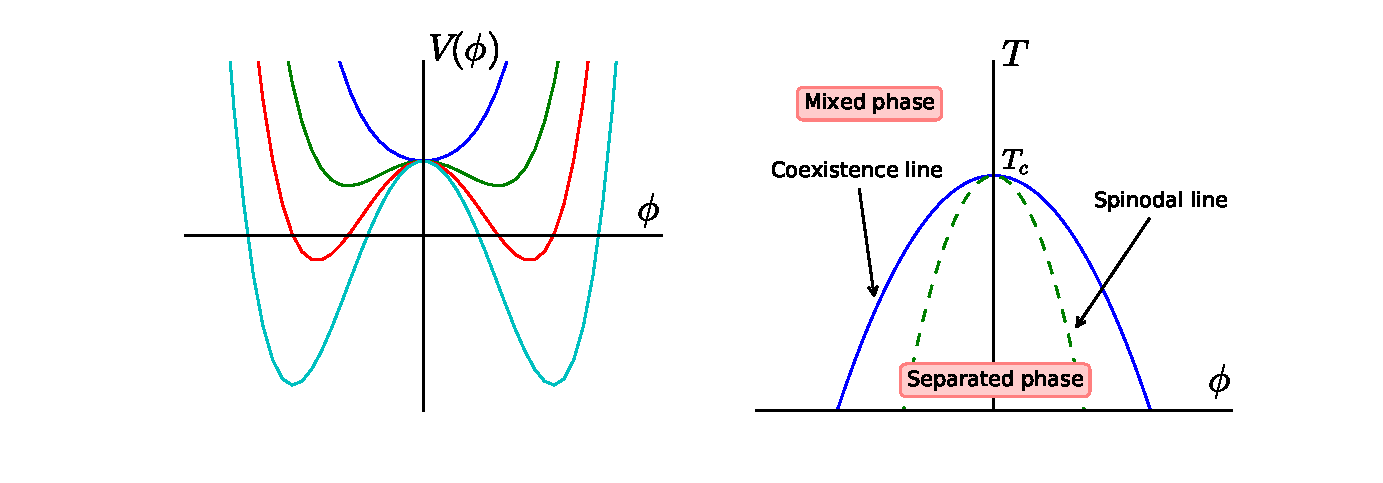
\includegraphics[width=0.9\textwidth]{figures/symmetric.eps}

\caption{Two panels showing (left) the form of the free energy density
$V(\phi)$ for the binary fluid for a number of different
temperatures. At temperatures above
the critical temperature, there is a single minimum (top curve), while
below $T_c$, two symmetric minima are present (lower curves). The related
phase diagram (right) in the temperature-composition plane shows mixed
and separated phases the boundary of which is the coexistence 
line. This (sometimes referred to as the binodal line) is the locus of
points which are the minima of $V(\phi)$ at different temperatures. The
spinodal line is formed by the locus of points which are the inflections
of $V(\phi)$.}
\label{figure-symmetric-schematic}
\end{figure}


If we consider a one-dimensional case, this is
\begin{equation}
A\phi + B\phi^3 - \kappa \frac{d^2 \phi}{dx^2} = 0.
\end{equation}
Note that the conservation of order parameter means this should be a
constrained minimisation, which can be handled by adding the
a Lagrange multiplier $\Lambda = \partial f / \partial \phi |_{\phi_0}$.
The resulting ordinary differential equation has a solution
$\phi(x) = \phi^\star \tanh(x/\xi)$ where $\xi$ is identified
as the interfacial width. It can be confirmed that this is a solution
if
\begin{equation}
\xi = (-2\kappa / A)^{1/2}.
\end{equation}
The one-dimensional case can also be used to determine the interfacial
tension, which is the excess energy associated with the interface.
If we denote the interfacial tension $\sigma$, then the excess
energy is
\begin{equation}
\sigma = \int_{-\infty}^{+\infty} \mathrm{d} x
\Big[
{\textstyle \frac{1}{2}} \kappa (d_x \phi)^2 + V(\phi) - V(\phi^\star)
\Big],
\end{equation}
which can be evaluated from the equilibrium profile with the interface
placed at the origin $\phi(x) = \phi^\star\tanh(x/\xi)$, along with a number
of standard integrals, to give
\begin{equation}
\sigma =  4\kappa\phi^{\star 2}/3\xi
 = \big(-8\kappa A^3/9B^2\big)^{1/2}.
\end{equation}
Further discussion of the practical choice of the free energy parameters,
and their
impact on interfacial width and tension is deferred until LATER.

\subsubsection{Dynamics}

In a purely diffusive regime, the time evolution of a conserved
order parameter may be expressed as the local divergence of a flux
$j_\alpha(\mathbf{r})$, that is,
$\partial_t \phi(\mathbf{r}) + \partial_\alpha j_\alpha(\mathbf{r}) = 0$.
In this picture, the system responds to small local changes in composition
by diffusion, which acts to reduce the energy. Formally, this
response of the free energy to a small change in composition is described
by the chemical potential
\begin{equation}
\mu = \frac{\delta F}{\delta \phi} = \frac{dV}{d\phi} - \kappa \partial_\alpha^2 \phi,
\end{equation}
being the functional derivative of the free energy with respect to the
order parameter. The dynamics is usually described in the context of the
model of Cahn and Hilliard \cite{cahn-hilliard-1958}, otherwise known as
Model B, where
\begin{equation}
\frac{\partial \phi}{\partial t} =
M\partial_\alpha^2 \frac{\delta F}{\delta \phi}.
\label{eq-cahn-hilliard}
\end{equation}
Here, the diffusive flux is related to the gradient of chemical potential
via $j_\alpha = -M \partial_\alpha \mu$, where $M$ is a mobilty
(taken to be uniform). 

In the presence of a fluid with velocity field $u_\alpha(\mathbf{r})$,
the full equation for the time evolution of the order parameter is
\begin{equation}
\partial_t \phi + \partial_\alpha (\phi u_\alpha + M\partial_\alpha \mu) = 0.
\label{eq-cahn-hilliard-final}
\end{equation}
This form again stresses the nature of the dynamics as a conservation law,
involving the divergence of advective fluxes $\phi u_\alpha$ and diffusive
fluxes $j_\alpha = -M\partial_\alpha \mu$. It
also admits that the mobility may be a function of position, e.g., via
$M = M(\phi)$. Equation~\ref{eq-cahn-hilliard-final} will form the basis of
the numerical solution of the binary fluid problem, coupled to the
Navier-Stokes equation.

The presence of a interface, or non-uniform composition, can lead to
thermodynamic stresses on the fluid which we denote $P_{\alpha\beta}$,
in additional to the usual viscous
stresses. The divergence of this
additional stress represents a body force density in the Navier-Stokes
equation, which is related to the chemical potential via
$f_\alpha = -\phi\partial_\alpha \mu = -\partial_\beta P_{\alpha\beta}$.
The full form of the additional stress may be related to the order
parameter by
\begin{equation}
P_{\alpha\beta} = p_0 \delta_{\alpha\beta}
  + \kappa \partial_\alpha \phi \partial_\beta \phi
\end{equation}
with isotropic contribution
\begin{equation}
p_0 = \phi \frac{dV(\phi)}{d\phi} -  V(\phi)
-\kappa\phi\partial_\alpha^2 \phi - \textstyle{\frac{1}{2}} \kappa (\partial_\alpha \phi)^2.
\end{equation}
Note that the stress $P_{\alpha\beta}$ is symmetric. At (local) equilibrium,
one expects gradients in the chemical potential to vanish,
and there will be neither diffusive fluxes ($j_\alpha = 0$) nor force on
the fluid ($f_\alpha = 0$).

\subsubsection{Surface (or wetting) free energy}

In the presence of a solid surface, the two component fluid gives
rise to the possiblity of a solid-fluid-fluid contact line. In the
symmetric case, the fluid-fluid interface will be at right angles to
a uniform flat surface. If one component wets the solid preferentially
(that is, it is energetically favourable for that component to be
in contact with the solid) the angle may move away from
90~degrees.
In general, the equilibrium contact angle $\theta$ is given by the
Young equation
\begin{equation}
\sigma_1 - \sigma_2 - \sigma \cos\theta = 0,
\end{equation}
where there are two solid-fluid surface tensions for components 1 and 2,
and the fluid-fluid interfacial tension is $\sigma$ as before.

This may be described in the free energy picture by adding a free
energy density per unit area assoicated with the surface:
\begin{equation}
f_s (\phi_s)= \textstyle{\frac{1}{2}} C \phi_s^2 + H \phi_s,
\end{equation}
where $\phi_s$ is the order parameter at the surface, and $C$ and $H$ are
constant parameters.

\subsection{Implementation}

\subsubsection{Lattice kinetic approach}

A second distribution function is introduced, denoted $g_i(\mathbf{r};t)$,
which describes the composition. The moments of this distribution, by
analogy with the hydrodynamic case with distribution
$f_i(\mathbf{r};t)$ given in
Eq.~\ref{equation-lb-f-moments}, are written
\begin{equation}
\phi(\mathbf{r};t) = \sum_i g_i (\mathbf{r};t), \quad
j_\alpha(\mathbf{r};t) = \sum_i g_i(\mathbf{r};t) c_{i\alpha}, \quad
\Phi_{\alpha\beta}(\mathbf{r};t) = \sum_i g_i(\mathbf{r};t)
c_{i\alpha}c_{i\beta}.
\end{equation}
Again, the summation is over index $i$ which counts the number of
discrete velocity components for the relevant lattice Boltzmann
model $N_{\mathrm{vel}}$. However, for the Cahn-Hilliard equation,
the only relevant physical moments are the order parameter
$\phi(\mathbf{r};t)$ and the flux $j_\alpha(\mathbf{r};t)$, so
the quantity $\Phi_{\alpha\beta}(\mathbf{r};t)$ is counted among
the kinetic modes and has no precise physical interpretation. In
contrast to the previous section, here $j_\alpha(\mathbf{r};t)$
is used to represent the total flux (advective
plus diffusive) rather than the purely diffusive flux.

The lack of direct physical interpretation for the second moment
means there are a number of possible choices at the collision
stage for the $g_i(\mathbf{r};t)$ distribution.
\begin{enumerate}
\item
Following Stratford \textit{et al.} \cite{j-stat-phys-2005}:
relax $j_\alpha$ toward the equilibrium $\phi u_\alpha$
at a rate related to the mobility and fix $\Phi_{\alpha\beta} =
\phi u_\alpha u_\beta + \mu \delta_{\alpha\beta}$.
\item
Following Kendon \textit{et al.} \cite{kendon2001}: fix both
$j_\alpha = \phi$ and
$\Phi_{} = \phi u_\alpha u_\beta + M\mu \delta_{\alpha\beta}$ so the
mobilty enters explicitly with the chemical potential.
\end{enumerate}

In both cases a reprojection is used to recover the post-collision
distributions $g_i^\star(\mathbf{r};t)$. This explicitly eliminates
kinetic modes other than $\Phi_{\alpha\beta}$. Hence
\begin{equation}
g_i = w_i \big(\phi + \phi u_\alpha c_{i\alpha}/c_s^2 +
(\mu\delta_{\alpha\beta} + \phi u_\alpha u_\beta) Q_{i\alpha\beta}/2c_s^4\big).
\end{equation}
In practice, this is not stable, and we use
\begin{equation}
g_i = \phi\delta_{i0} + w_i \big( j_\alpha c_{i\alpha} / c_s^2
+ \Phi_{\alpha\beta}Q_{i\alpha\beta} / 2c_s^4\big)
\end{equation}
where the $\delta_{i0}$ has the effect of moving most of the order
parameter into the non-propagating rest distribution $g_0$. 
This reprojection approach has the advantage that it eliminates several
spurious anisotropic terms which are introduced by a single relaxation
time approach (used by Kendon \textit{et al.}).

In the relaxation approach, the form of the relaxation for the
three components of the order parameter flux is
\begin{equation}
j_\alpha^\star =
j_\alpha - \tau_\phi^{-1} (j_\alpha - \phi u_\alpha),
\end{equation}
where $j_\alpha^\star$ is the post-collision flux and the relaxation
time $\tau_\phi$ is related to the mobility  via
\begin{equation}
\tau = {\textstyle\frac{1}{2}} + M\rho_0/\Delta t.
\end{equation}

\subsubsection{Finite difference approach}

For a number of reasons, it is advantageous to replace the lattice
kinetic approach by a conventional finite difference/finite volume
treatment of the Cahn-Hilliard equation
\begin{equation}
\partial_t \phi + \partial_\alpha ( \phi u_\alpha - M \partial_\alpha \mu) = 0.
\end{equation}
(Note that the finite difference and finite volume terminology will
be used somewhat interchanably here.) Briefly, the advantages are:
\begin{enumerate}
\item
The ambiguity in interpretation of the kinetic modes is avoided,
along with the corresponding computational overhead in memory and
memory movement.
\item
Additional features may be added to the Cahn-Hilliard equation more
easily. These might include a heterogeneous mobility $M=M(\phi)$, and
order parameter fluctuations (see below).
\end{enumerate}

\vfill
\pagebreak

%%%%%%%%%%%%%%%%%%%%%%%%%%%%%%%%%%%%%%%%%%%%%%%%%%%%%%%%%%%%%%%%%%%%%%%%%%%%%%%
%
%  liquidcrystal.tex
%
%  For nematics, cholesterics, blue phases based on the Landau
%  de Gennes approach.
%
%  Edinburgh Soft Matter and Statistical Physics Group and
%  Edinburgh Parallel Computing Centre
%
%  Contributing authors:
%  Kevin Stratford (kevin@epcc.ed.ac.uk)
%  Davide Marenduzzo was the source of the original LC approach.
%
%%%%%%%%%%%%%%%%%%%%%%%%%%%%%%%%%%%%%%%%%%%%%%%%%%%%%%%%%%%%%%%%%%%%%%%%%%%%%%%

\section{Liquid Crystals}
\label{section-lc}

\subsection{The Landau-de Gennes Approach}

\subsubsection{Tensor order parameter}

The liquid crystal order is described by a symmetric traceless tensor
$Q_{\alpha\beta}(\mathbf{r}; t)$. The largest eigenvalue and
associated eigenvector of $Q_{\alpha\beta}$ represent the magnitude
and local direction of liquid crystal molecular order. A theory based
on the tensor $Q_{\alpha\beta}$ has the advantage of being able to
describe disclinations where the local order vanishes and a director
is not defined. Readers are referred to, e.g., de Gennes and Prost
\cite{degennes-prost2002}, and Wright and Mermin \cite{wright-mermin}
for further information.

\subsubsection{Free Energy Density}

The free energy is a functional whose density
$f(Q_{\alpha\beta}, \partial_\gamma Q_{\alpha\beta})$
has bulk contributions depending on $Q_{\alpha\beta}$,
and elastic (distortion) contributions dependent on the
gradients of the order parameter
$\partial_\gamma Q_{\alpha\beta}$.

The bulk contributions are
\begin{equation}
\label{eq-lc-fed-bulk}
f(Q_{\alpha\beta}) =
{\textstyle\frac{1}{2}} A_0 (1 - \gamma / 3) Q_{\alpha\beta}^2
-{\textstyle\frac{1}{3}} A_0 \gamma Q_{\alpha\beta} Q_{\beta\pi} Q_{\pi\alpha}
+ {\textstyle\frac{1}{4}} A_0 \gamma (Q_{\alpha\beta}^2)^2.
\end{equation}
Here, $A_0$ is a constant which sets the overall energy scale; $\gamma$
is a temperature-like parameter which controls the position in the
phase diagram relative to the isotropic-nematic transition.

The bend, splay and twist distortions making up the gradient free
energy are modelled with two elastic
constants $\kappa_0$ and $\kappa_1$ as
\begin{equation}
f(\partial_\gamma Q_{\alpha\beta}) = 
{\textstyle\frac{1}{2}} \kappa_0 (\partial_\alpha Q_{\alpha\beta})^2
+ {\textstyle\frac{1}{2}} \kappa_1
(\epsilon_{\alpha\mu\nu} \partial_\mu Q_{\nu\beta} + 2q_0 Q_{\alpha\beta})^2.
\label{equation-lc-gradient-fe}
\end{equation}
Here, $\epsilon_{\alpha\mu\nu}$ is the permutation tensor and
$q_0 = 2\pi/p$ is a wavevector related to the pitch~$p$ of the
cholesteric. Setting $q_0 = 0$ permits a nematic state.
The one-constant approximation makes the simplification that
$\kappa_0 = \kappa_1 = \kappa$; the distinction between
$\kappa_0$ and $\kappa_1$ will be kept
in what follows unless otherwise stated.


\subsubsection{Molecular Field}

The molecular field $H_{\alpha\beta}$ is defined as the functional
derivative of the
free energy density with respect to the order parameter which here
gives
\begin{equation}
H_{\alpha\beta} = -\Bigg[
  \frac{\partial f(Q_{\alpha\beta})}{\partial Q_{\alpha\beta}}
- \partial_\gamma \frac{\partial f(\partial_\gamma Q_{\alpha\beta})}
{\partial Q_{\alpha\beta,\gamma}} \Bigg].
\end{equation}
In the absence of flow, the molecular field determines how the
order parameter relaxes toward equilibrium.

As the final expression for $H_{\alpha\beta}$ is somewhat complex, it
is useful to 
account for the individual terms here. First, the terms from the bulk free
energy density give rise to:
\begin{equation}
-A_0 (1 - \gamma/3) Q_{\alpha\beta} + A_0 \gamma Q_{\alpha\pi} Q_{\pi\beta}
- A_0 \gamma Q_{\pi\sigma}^2 Q_{\alpha\beta}.
\nonumber
\end{equation}
The second term in this expression
(arising from the cubic term in the free energy) is
forced to be traceless by subtracting one third of
Tr$(Q_{\alpha\pi}Q_{\pi\beta}) = Q_{\alpha\beta}^2$
so that we have
\begin{equation}
- A_0 (1 - \gamma/3) Q_{\alpha\beta}
+ A_0 \gamma (Q_{\alpha\pi} Q_{\pi\beta}
               - {\textstyle\frac{1}{3}} Q_{\pi\sigma}^2\delta_{\alpha\beta})
- A_0 \gamma Q_{\pi\sigma}^2 Q_{\alpha\beta}.
\nonumber
\end{equation}

The gradient term in $\kappa_0$, along with the first term in $\kappa_1$
arising from the expansion of the brackets in
Equation~\ref{equation-lc-gradient-fe}, give
\begin{equation}
\kappa_0 \partial_\alpha \partial_\gamma Q_{\gamma\beta}.
+
\kappa_1 \partial_\gamma
( \partial_\gamma Q_{\alpha\beta} - \partial_\alpha Q_{\gamma\beta}).
\nonumber
\end{equation}
Note that in the one constant approximation, this term collapses
to $\kappa \partial^2 Q_{\alpha\beta}$. The cross term in the expansion
of the brackets in~\ref{equation-lc-gradient-fe}, having been symmetrised,
contributes
\begin{equation}
-2\kappa_1 q_0
( \epsilon_{\alpha\mu\nu} \partial_\mu Q_{\nu\beta}
+ \epsilon_{\beta\mu\nu} \partial_\mu Q_{\nu\alpha}),
\nonumber
\end{equation}
which must again be forced to be traceless to give
\begin{equation}
-2\kappa_1 q_0 \big\{
( \epsilon_{\alpha\mu\nu} \partial_\mu Q_{\nu\beta}
+ \epsilon_{\beta\mu\nu} \partial_\mu Q_{\nu\alpha})
- {\textstyle\frac{1}{3}}( 
   \epsilon_{\pi\mu\nu} \partial_\mu Q_{\nu\pi}
  +\epsilon_{\pi\mu\nu} \partial_\mu Q_{\nu\pi} )
   \delta_{\alpha\beta} \big\}.
\nonumber
\end{equation}
The final term in is
$-4 \kappa_1 q_0^2 Q_{\alpha\beta}$. The complete expression for the molecular
field is then
\begin{eqnarray}
\label{eq-lc-h-full}
H_{\alpha\beta} &=&
- A_0 (1 - \gamma/3) Q_{\alpha\beta}
+ A_0 \gamma (Q_{\alpha\pi} Q_{\pi\beta}
               - {\textstyle\frac{1}{3}} Q_{\pi\sigma}^2\delta_{\alpha\beta})
- A_0 \gamma Q_{\pi\sigma}^2 Q_{\alpha\beta}
\nonumber\\
&&
+\kappa_0 \partial_\alpha \partial_\gamma Q_{\gamma\beta}
+
\kappa_1 \partial_\gamma
( \partial_\gamma Q_{\alpha\beta} - \partial_\alpha Q_{\gamma\beta})
\nonumber\\
&&
-2\kappa_1 q_0 \big(
( \epsilon_{\alpha\mu\nu} \partial_\mu Q_{\nu\beta}
+ \epsilon_{\beta\mu\nu} \partial_\mu Q_{\nu\alpha})
- {\textstyle\frac{1}{3}}( 
   \epsilon_{\pi\mu\nu} \partial_\mu Q_{\nu\pi}
  +\epsilon_{\pi\mu\nu} \partial_\mu Q_{\nu\pi} )
   \delta_{\alpha\beta} \big)
\nonumber\\
&& - 4 \kappa_1 q_0^2 Q_{\alpha\beta}.
\end{eqnarray}


\subsection{Surface Anchoring}

\label{section-lc-anchoring}

The preferred orientation of the liquid crystal fluid at a solid surface,
usually referred to as the surface anchoring, is relevant for both
solid walls and colloids.

\subsubsection{General boundary condition}

To impose a suitable boundary condition for the order parameter tensor
at a solid-fluid interface, we consider again the gradient terms in
the free energy
\begin{equation}
f (\partial_\gamma Q_{\alpha\beta}) = 
{\textstyle\frac{1}{2}} \kappa_0 (\partial_\beta Q_{\alpha\beta})^2
+ {\textstyle\frac{1}{2}}
 \kappa_1 (\epsilon_{\alpha\gamma\sigma} \partial_\gamma
Q_{\sigma\beta} + 2q_0 Q_{\alpha\beta})^2
\end{equation}
where we retain
two elastic constants $\kappa_0$ and $\kappa_1$;
the cholesteric pitch $p = 2\pi/q_0$.

Also relevant is a surface free energy (an area density), the exact form
of which is determined by the type of anchoring required. In general, we
expect this to depend on the order parameter, but not its gradients, so
write
\begin{equation}
f_s = f_s (Q_{\alpha\beta}, Q^0_{\alpha\beta})
\end{equation}
where $Q^0_{\alpha\beta}$ is some preferred order parameter configuration
at the surface (to be either normal or planar as discussed in the following
sections).

The boundary condition we wish to apply is derived from the Euler-Lagrange
equations, and for the fluid and surface terms gives rise to the equation
\begin{equation}
n_\gamma \frac{\partial f}{\partial Q_{\alpha\beta,\gamma}}
+ \frac{\partial f_s}{\partial Q_{\alpha\beta}} = 0,
\label{equation-lc-general-bc}
\end{equation}
where $n_\gamma$ is the outward unit normal at the surface (pointing into
the fluid). Note that the first term in the derivative of the fluid free
energy term with respect to
$Q_{\alpha\beta,\gamma}$ can be expended as
\begin{equation}
\kappa_0 n_\beta \partial_\gamma Q_{\alpha\gamma}
+ \kappa_1 n_\gamma
(\partial_\gamma Q_{\alpha\beta} - \partial_\alpha Q_{\gamma\beta})
- 2\kappa_1 q_0 n_\gamma \epsilon_{\alpha\gamma\sigma} Q_{\sigma\beta}.
\nonumber
\end{equation}
However, we should use a symmetric form (the derivative with respect to
$Q_{\beta\alpha,\gamma}$ is just as good) so we write this as:
\begin{eqnarray}
&
{\textstyle\frac{1}{2}} \kappa_0 (n_\alpha \partial_\gamma Q_{\beta\gamma}
+ n_\beta \partial_\gamma Q_{\alpha\gamma})
+ \kappa_1 n_\gamma \partial_\gamma Q_{\alpha\beta}
- {\textstyle\frac{1}{2}} \kappa_1 n_\gamma ( \partial_\alpha Q_{\gamma\beta}
+ \partial_\beta Q_{\gamma\alpha})
\nonumber
\\
&
- \kappa_1 q_0 n_\gamma (\epsilon_{\alpha\gamma\sigma} Q_{\sigma\beta}
+ \epsilon_{\beta\gamma\sigma}Q_{\sigma\alpha}).
\nonumber
\end{eqnarray}
The exact boundary condition will contain this term plus one
depending on the exact choice of the surface free energy which
describes a given anchoring condition.

\subsubsection{Normal or homeotropic anchoring}
The preferred direction of the surface order here is, as the name
suggests, normal to surface. We can write
\begin{equation}
f_s = {\textstyle\frac{1}{2}} w (Q_{\alpha\beta} - Q_{\alpha\beta}^0)^2
\end{equation}
where $w$ is a constant.
The preferred orientation $Q^0_{\alpha\beta}$ is based on the unit normal
at the surface $n_\gamma$, and is computed via the uniaxial approximation:
\begin{equation}
Q^0_{\alpha\beta}
= {\textstyle \frac{1}{2}} A (3n_\alpha n_\beta - \delta_{\alpha\beta}).
\end{equation}
The amplitude $A$ is provided by 
\begin{equation}
\label{equation-lc-amplitude}
A=\frac{2}{3}\left(\frac{1}{4}+\frac{3}{4}\sqrt{1 - \frac{8}{3\gamma}}\right).
\end{equation}
The full boundary condition for the gradient of the tensor order parameter
at the solid-fluid boundary from Equation~\ref{equation-lc-general-bc}
is then:
\begin{eqnarray}
{\textstyle\frac{1}{2}} \kappa_0 (n_\alpha \partial_\gamma Q_{\beta\gamma}
+ n_\beta \partial_\gamma Q_{\alpha\gamma})
+ \kappa_1 n_\gamma \partial_\gamma Q_{\alpha\beta}
- {\textstyle\frac{1}{2}} \kappa_1 n_\gamma ( \partial_\alpha Q_{\gamma\beta}
+ \partial_\beta Q_{\gamma\alpha})
\nonumber
\\
- \kappa_1 q_0 n_\gamma (\epsilon_{\alpha\gamma\sigma} Q_{\sigma\beta}
+ \epsilon_{\beta\gamma\sigma}Q_{\sigma\alpha})
- w(Q_{\alpha\beta} - Q_{\alpha\beta}^0) = 0.
\label{equation-lc-bc-normal}
\end{eqnarray}

\subsubsection{Planar (degenerate) anchoring}

For planar anchoring, the preferred orientation is in the local tangent
plane at the surface: this is a degenerate case as any orientation in
the plane is energetically equivalent. An appropriate boundary
condition is described by Fournier and Galatola \cite{fournier2005}
which we write as:
\begin{equation}
f_s =
{\textstyle\frac{1}{2}} w_1 (\tilde{Q}_{\alpha\beta} - \tilde{Q}^\perp_{\alpha\beta})^2
+ {\textstyle\frac{1}{2}} w_2 (\tilde{Q}_{\alpha\beta}^2 - A^2)^2.
\end{equation}
Here again, the amplitude $A$ is provided by
Equation~\ref{equation-lc-amplitude}. To compute this term we take
the local fluid order parameter $Q_{\alpha\beta}$, form the quantity
$$
\tilde{Q}_{\alpha\beta}
= Q_{\alpha\beta} + {\textstyle \frac{1}{2}A\delta_{\alpha\beta} }
$$
which is then projected onto the tangent plane via
$
\tilde{Q}^\perp_{\alpha\beta}
= P_{\alpha\gamma} \tilde{Q}_{\gamma\sigma} P_{\sigma\beta}
$
with the local surface normal entering through
$P_{\alpha\beta} = \delta_{\alpha\beta} - n_\alpha n_\beta$.
The full boundary condition resulting from
Equation~\ref{equation-lc-general-bc} is then
\begin{eqnarray}
{\textstyle\frac{1}{2}} \kappa_0 (n_\alpha \partial_\gamma Q_{\beta\gamma}
+ n_\beta \partial_\gamma Q_{\alpha\gamma})
+ \kappa_1 n_\gamma \partial_\gamma Q_{\alpha\beta}
- {\textstyle\frac{1}{2}} \kappa_1 n_\gamma ( \partial_\alpha Q_{\gamma\beta}
+ \partial_\beta Q_{\gamma\alpha})
\nonumber
\\
- \kappa_1 q_0 n_\gamma (\epsilon_{\alpha\gamma\sigma} Q_{\sigma\beta}
+ \epsilon_{\beta\gamma\sigma}Q_{\sigma\alpha})
- w_1 (\tilde{Q}_{\alpha\beta} - \tilde{Q}_{\alpha\beta}^\perp)
- 2w_2(\tilde{Q}_{\alpha\beta}^2 - A^2)\tilde{Q}_{\alpha\beta} = 0.
\label{equation-lc-bc-planar}
\end{eqnarray}



\subsection{Dynamics}

The time evolution of the orientational order parameter $Q_{\alpha\beta}$
in the presence of flow can be described by the Beris-Edwards equation
\cite{beris-edwards}.

\begin{equation}
\partial_t Q_{\alpha\beta} + \partial_\gamma (u_\gamma Q_{\alpha\beta})
+ S_{\alpha\beta}(W_{\alpha\beta}, Q_{\alpha\beta}) = -\Gamma  H_{\alpha\beta}.
\label{equation-lc-beris-edwards}
\end{equation}
This relates the time rate of change of the order parameter to terms
involving advection, the response to shear
$S_{\alpha\beta}(W_{\alpha\beta},Q_{\alpha\beta})$, and the molecular
field.

The advective term involves the fluid velocity $u_\alpha$ and the shear
term involves the velocity gradient tensor
$W_{\alpha\beta}= \partial_\beta u_\alpha$. The full definition of the
shear term is:
\begin{eqnarray}
S_{\alpha\beta} (W_{\alpha\beta}, Q_{\alpha\beta})
& = 
(\xi D_{\alpha\pi} + \Omega_{\alpha\pi})
(Q_{\pi\beta} + {\textstyle \frac{1}{3}} \delta_{\pi\beta})
+
(Q_{\alpha\pi} + {\textstyle \frac{1}{3}} \delta_{\alpha\pi})
(\xi D_{\pi\beta} - \Omega_{\pi\beta})
\nonumber\\
&-
2\xi(Q_{\alpha\beta} + {\textstyle\frac{1}{3}}\delta_{\alpha\beta})
Q_{\pi\sigma}W_{\sigma\pi}
\nonumber
\end{eqnarray}
where $D_{\alpha\beta} = \frac{1}{2}(W_{\alpha\beta} + W_{\beta\alpha})$ and
 $\Omega_{\alpha\beta} = \frac{1}{2}(W_{\alpha\beta} - W_{\beta\alpha})$
are the symmetric and antisymmetric contributions to the velocity gradient
tensor and $\xi$ is a material constant representing an effective
molecular aspect ratio.


The thermodynamic contribution to the stress on the fluid can be viewed as
the sum of three parts:
\begin{equation}
\Pi_{\alpha\beta} = \sigma_{\alpha\beta} + \tau_{\alpha\beta}
-
\partial_\alpha Q_{\pi\nu}
\frac{\delta {\cal F}}{ \delta \partial_\beta Q_{\pi\nu}}
\label{equation-lc-stress}
\end{equation}
where $\sigma_{\alpha\beta}$ and $\tau_{\alpha\beta}$ are the symmetric
and antisymmetric contributions from the liquid crystal order:
\begin{equation}
\sigma_{\alpha\beta} =
-p_0 \delta_{\alpha\beta} 
- \xi H_{\alpha\pi}(Q_{\pi\beta} + {\textstyle\frac{1}{3}}\delta_{\pi\beta})
- \xi (Q_{\alpha\pi} + {\textstyle\frac{1}{3}}\delta_{\alpha\pi}) H_{\pi\beta}
+ 2\xi (Q_{\alpha\beta} + {\textstyle \frac{1}{3}}\delta_{\alpha\beta} )
Q_{\pi\nu} H_{\pi\nu},
\end{equation}
where $p_0$ is the isotropic pressure, and
\begin{equation}
\tau_{\alpha\beta} = Q_{\alpha\pi} H_{\pi\beta} - H_{\alpha\pi} Q_{\pi\beta}. 
\end{equation}
The final term in Equation~\ref{equation-lc-stress} is expanded as
$$
-\kappa_0 \partial_\alpha Q_{\pi\beta} \partial_\nu Q_{\pi\nu}
-\kappa_1 \partial_\alpha Q_{\pi\nu}
\left[ \partial_\beta Q_{\pi\nu} - \partial_\pi Q_{\nu\beta}
+ 2q_0 \epsilon_{\gamma\beta\pi} Q_{\gamma\nu} \right].
$$


\subsubsection{Active stress}

An additional term may be added to the stress to model an active
apolar fluid. This term is
\begin{equation}
\Pi_{\alpha\beta}^a = -\zeta
(Q_{\alpha\beta} - {\textstyle\frac{1}{3}}\delta_{\alpha\beta})
\end{equation}
where $\zeta$ is an activity parameter: $\zeta < 0$ gives
contractile behaviour and $\zeta > 0$ gives extensile behaviour.

\subsection{Implementation}

\subsubsection{Fluid}

The time evolution of the order parameter is computed by a hybrid
approach where the hydrodynamics is in the LB sector, and the
Beris-Edwards Equation is solved in a finite difference approach.
The hydrodynamic quantities and the order parameter share the same
regular lattice. The velocity field, computed via LB, supplies
advective fluxes and the velocity gradient tensor using an appropriate
finite difference stencil.

Coupling to the Navier-Stokes equations is via a body force computed
locally at each lattice site via the divergence of the stress in
Equation~\ref{equation-lc-stress}.

It is also possible to compute solely relaxational dynamics where there
is no flow, and evolution only depends on the molecular field, and the
rotational diffusion constant.


\subsubsection{Solid}

First, we note that the assignment of solid and fluid lattice
nodes for the order parameter follows that for the density:
inside and outside are distinguished using the nominal radius
of the colloid $a_0$ and its position. It is useful, in addition,
to think about a series of control volumes surrounding each lattice
node whose faces are aligned with the lattice
(see Figure~\ref{figure-lc-hybrid}). A set of these
faces constitute the solid-fluid boundary in the hybrid picture.
Advective fluxes of order parameter are computed at the faces
of the control volumes, and the boundary condition is zero
normal flux at solid-fluid interfaces. Note that the colloid
is assumed to be stationary in assigning these fluxes.

\begin{figure}[h]
\begin{center}
%%%%%%%%%%%%%%%%%%%%%%%%%%%%%%%%%%%%%%%%%%%%%%%%%%%%%%%%%%%%%%%%%%%%%%%%%%%%%
%
%  hybrid.tex
%
%  Description of  LB-FD hybrid considerations.
%
%%%%%%%%%%%%%%%%%%%%%%%%%%%%%%%%%%%%%%%%%%%%%%%%%%%%%%%%%%%%%%%%%%%%%%%%%%%%%

\section{BBL and hybrid dynamics}

[I assume this will be preceded by some description of the
governing equations for the tensor order parameter and their
treatment.]

The well-established procedure of bounce-back on links (BBL)
\cite{Ladd04, nguyen} has been employed for the representation
of the colloids as moving solid objects within the LBM.
In the hybrid LB/FD approach used here, BBL is retained for
the distributions, which are simply reflected at the solid-fluid
surface with a correction which depends on the local surface
velocity (see Figure Xa). The resulting change in momentum is
summed over the links to give the net hydrodynamic
force on the colloid, which is then used to update the
particle velocity, and
hence position, in a molecular dynamics-like step. Boundary
conditions for the finite difference equations for the order
parameter tensor are dealt with in a different way.

First, we note that the assignment of solid and fluid lattice
nodes for the order parameter follows that for the density:
inside and outside are distinguished using the nominal radius
of the colloid $a_0$ and its position. It is useful, in addition,
to think about a series of control volumes surrounding each lattice
node whose faces are aligned with the lattice (Figure Xb). A set of
these
faces constitute the solid-fluid boundary in the hybrid picture.

Boundary conditions for $Q_{\alpha\beta}$ are of two types:
homeotropic, where the director  $n_\alpha^0$ is aligned with
the local unit normal to the surface $\hat{n}_\alpha$, and planar,
where the director lies in the plane of the tangent to the
surface. For either choice of director at the surface, we
may set the corresponding value of $Q_{\alpha\beta}$ at
lattice nodes immediately inside the surface via
\begin{equation}
Q_{\alpha\beta}^0 = S^0 (n_\alpha^0 n_\beta^0
- {\scriptstyle\frac{1}{3}}\delta_{\alpha\beta})
\end{equation}
where the constant $S^0$ controls the degree of surface order.
This allows us
to compute, at all fluid nodes, the derivatives
$\nabla_\gamma Q_{\alpha\beta}$ and $\nabla^2 Q_{\alpha\beta}$
using the same finite difference stencil. This allows the
molecular field and hence the diffusive terms in the Beris
Edwards equation to be computed.

Also appearing in the Beris-Edwards equations is the velocity
gradient tensor, which can be handled in a similar fashion
close to the colloid. The velocity field at solid nodes
immediately inside the colloid surface are set to the solid
body velocity $\bf{u} + \bf{\Omega} \times \bf{r}$. Again,
the velocity gradient tensor $\partial_\alpha u_\beta$ may
be computed using the same stencil at all fluid nodes.

Advective fluxes of order parameter are computed at the faces
of the control volumes, and the boundary condition is zero
normal flux at solid-fluid interfaces. Note that the colloid
is assumed to be stationary in assigning these fluxes.

The force on the fluid originating from the order parameter
is computed via the discrete divergence of the stress
$P_{\alpha\beta}$. In the fluid, this is implemented by
interpolating $P_{\alpha\beta}$ to the control volume faces
and taking differences between faces in each direction. This
method has the advantage that, with the introduction of colloids,
an interpolation/extrapolation of $P_{\alpha\beta}$ to the
solid-fluid boundary is possible. This allows one to compute the
divergence of the stress at fluid nodes adjacent to the colloid
in the normal way. At the same time, the discrete equivalent of
\begin{equation}
F_\alpha^\mathrm{coll} = \int P_{\alpha\beta} \hat{n}_\beta dS
\end{equation}
by summing $P_{\alpha\beta}$ over the relevant solid-fluid control
volume faces. By construction, this ensures that momentum lost by
the fluid is gained by the colloid, i.e., global momentum is
conserved.

Finally, movement of the colloid across the lattice is accompanied
by changes in its discrete shape. The events necessitate the
removal or replacement of fluid information. For the replacement
of fluid at newly exposed lattice nodes, this means an
interpolation of nearby order parameter values in the fluid to
provide the new information. This is analogous to what is done
for the LB distributions.


\begin{figure}[h]
\begin{center}

%\input{/home/kevin/doc/rgrid/xfig/hybrid1.epic}
\input{hybrid2.epic}
\end{center}
\caption{The colloid (represented by the solid circle) moves continuously
across the lattice. Lattice sites inside are designated solid, and those
outside fluid (open and closed points, respectively). In the lattice
Boltzmann picture (left) the surface is defined by a set of links
$f_b$, which involve discrete vectors $\mathbf{c}_b \Delta t$ which
connect fluid and solid sites. For the order parameter (right), the
colloid is represented by the set of faces, e.g., that between sites
$i,j$ and $i+1,j$ with unit normal $\hat{n_x}$. Discretisation effects
are found to be negigible for radii greater than about 5 lattice units.}
\end{figure}

\end{center}
\caption{The hybrid picture. In the lattice
Boltzmann picture (left) a surface is defined by a set of links
$f_b$, which involve discrete vectors $\mathbf{c}_b \Delta t$ which
connect fluid and solid sites. For the order parameter (right), the
colloid is represented by the set of faces, e.g., that between sites
$i,j$ and $i+1,j$ with unit normal $\hat{n}_x$. This is a rather small
colloid.}
\label{figure-lc-hybrid}
\end{figure}

The net hydrodynamic force on the colloid is computed via BBL
in the usual way. As discussed above, the force on the fluid
originating from the order parameter is computed via the
discrete divergence of the stress $\Pi_{\alpha\beta}$. In the
fluid, this is implemented by interpolating $\Pi_{\alpha\beta}$
to the control volume faces and taking differences between faces
in each direction. This method has the advantage that, with the
introduction of solid faces, an extrapolation of $\Pi_{\alpha\beta}$
to the solid-fluid boundary is possible. This allows one to compute
the divergence of the stress at fluid nodes adjacent to the colloid
in the normal way. At the same time, the discrete equivalent of
\begin{equation}
F_\alpha^\mathrm{coll} = \int \Pi_{\alpha\beta} \hat{n}_\beta dS
\end{equation}
may be found by summing $\Pi_{\alpha\beta}$ over the relevant solid-fluid
control volume faces. By construction, this ensures that momentum lost by
the fluid is gained by the colloid, i.e., global momentum is
conserved.

Finally, movement of the colloid across the lattice is accompanied
by changes in its discrete shape. When fluid sites are destroyed,
corresponding order parameter information is also lost. If new
fluid sites are created, new order parameter information may be
added locally either by interpolation from nearby fluid sites, or
from geometrical information from the local surface anchoring.


\subsubsection{Boundary conditions}

\begin{table}[t]
\centering
\tabcolsep=4pt
\begin{tabular}{|c|cccccc|}
\hline
&
$Q_{xx,x}$ & $Q_{xy,x}$ & $Q_{xz,x}$ & $Q_{yy,x}$ & $Q_{yz,x}$ & $Q_{zz,x}$\\
\hline
$Q_{xx}$ &
$\kappa_0 n_x$ & $-\kappa_1 n_y$ & $-\kappa_1 n_z$ & & &\\
$Q_{xy}$ &
$\kappa_0 n_y$ & $\kappa' n_x$ & & $-\kappa_1 n_y$  & $-\kappa_1 n_z$ & \\
$Q_{xz}$ &
$\kappa_0 n_z$ & & $\kappa' n_x$ & & $-\kappa_1 n_y$ &$ -\kappa_1 n_z$\\
$Q_{yy}$ &
 & $\kappa_0 n_y$ & & $\kappa_1 n_x$ & &\\
$Q_{yz}$ &
 & $\kappa_0 n_z$ & $\kappa_0 n_y$ & & $2\kappa_1 n_x$ & \\
$Q_{zz}$ &
 & & $\kappa_0 n_z$ & & & $\kappa_1 n_x$\\
\hline
\hline
&
$Q_{xx,y}$ & $Q_{xy,y}$ & $Q_{xz,y}$ & $Q_{yy,y}$ & $Q_{yz,y}$ & $Q_{zz,y}$\\
\hline
$Q_{xx}$ &
$\kappa_1 n_y$ & $\kappa_0 n_x$ & & & &\\
$Q_{xy}$ &
$-\kappa_1 n_x$ & $\kappa' n_y$ & $-\kappa_1 n_z$ & $\kappa_0 n_x$ & &\\
$Q_{xz}$ &
 & $\kappa_0 n_z$ & $2\kappa_1 n_y$ & & $\kappa_0 n_x$ & \\
$Q_{yy}$ &
 & $-\kappa_1 n_x$ & & $\kappa_0 n_y$ & $-\kappa_1 n_z$ & \\
$Q_{yz}$ &
 & & $-\kappa_1 n_x$ & $\kappa_0 n_z$ & $\kappa' n_y$ & $-\kappa_1 n_z$\\
$Q_{zz}$ &
 & & & & $\kappa_0 n_z$ & $\kappa_1 n_y$\\
\hline
\hline
&
$Q_{xx,z}$ & $Q_{xy,z}$ & $Q_{xz,z}$ & $Q_{yy,z}$ & $Q_{yz,z}$ & $Q_{zz,z}$\\
\hline
$Q_{xx}$ &
$\kappa_1 n_z$ & & $\kappa_0 n_x$ & & & \\
$Q_{xy}$ &
 & $2\kappa_1 n_z$ & $\kappa_0 n_y$ & & $\kappa_0 n_x$ & \\
$Q_{xz}$ &
$-\kappa_1 n_x$ & $-\kappa_1 n_y$ & $\kappa' n_z$ & & & $\kappa_0 n_x$  \\
$Q_{yy}$ &
 & & & $\kappa_1 n_z$ & $\kappa_0 n_y$ & \\
$Q_{yz}$ &
 & $-\kappa_1 n_x$ & & $-\kappa_1 n_y$ & $\kappa' n_z$ & $\kappa_0 n_y$ \\
$Q_{zz}$ &
 & & $-\kappa_1 n_x$ & & $-\kappa_1 n_y $ & $\kappa_0 n_z$\\
\hline
\end{tabular}
\caption{Coefficients of the various derivatives of the order parameter
tensor appearing in six equations for the elements of the
order parameter (including $Q_{zz}$).
Note $\kappa_0 + \kappa_1 = \kappa'$ and all the
coefficients have been multiplied by a factor of 2 in the off-diagonal
equations.}
\label{table-lc-bc}
\end{table} 


In three dimensions, the boundary condition Eq.~\ref{equation-lc-general-bc}
provides six equations containing (potentially) 18 unknown derivatives
$\partial_\gamma Q_{\alpha\beta}$
corresponding to the 6 elements of the order parameter
tensor $Q_{xx}$, $Q_{xy}$, $Q_{xz}$, $Q_{yy}$, $Q_{yz}$, $Q_{zz}$.
While the equation corresponding to $Q_{zz}$ must appear to
retain isotropy, $Q_{zz}$ itself, and its derivatives, may be
replaced via the
constraint on the trace of $Q_{\alpha\beta}$. We can therefore either
solve a fully determined system including $Q_{zz}$, and then impose
tracelessness on the result, or replace $Q_{zz}$ and solve six
equations for five unknowns, with the sixth equation acting as the
constraint. These methods provide the same answer for cases where
the surface normal is along the coordinate directions.

In general, Equation~\ref{equation-lc-general-bc} is slightly
cumbersome: the coefficients of the various derivatives for each
of the six equations are shown in Table~\ref{table-lc-bc}. As an
concrete example,
at a flat surface with normal anchoring and, e.g., $n = (1, 0, 0)$,
the number of unknowns (six) are the gradients $\partial_x Q_{\alpha\beta}$
at the boundary --- we assume the tangential gradients
$\partial_y Q_{\alpha\beta}$
and $\partial_z Q_{\alpha\beta}$ can be approximated
using the standard differencing method involving only fluid values of
$Q_{\alpha\beta}$. We proceed by
computing the constant terms relevant for normal anchoring
$$
- \kappa_1 q_0 n_\gamma (\epsilon_{\alpha\gamma\sigma} Q_{\sigma\beta}
+ \epsilon_{\beta\gamma\sigma}Q_{\sigma\alpha})
- w(Q_{\alpha\beta} - Q_{\alpha\beta}^0)
$$
using $Q_{\alpha\beta}$ from the adjacent fluid site. To these
constant terms are added the tangential gradients.
The gradients at the surface are then computed by solving a 6x6
linear algebra problem for $\partial_x Q_{\alpha\beta}$. This
allows the full gradient at the adjacent fluid site to be constructed.

At concave edges or corners, where it is not possible to compute the
tangential gradients from the usual stencil as for a flat interface,
a different approach is required. Here, either a 12$\times$12 or
18$\times$18 system of equations is solved containing the relevant
unknown coefficients from Table~\ref{table-lc-bc} and the relevant
constant terms computed as before.





\vfill
\pagebreak

\section{Electrokinetics}

\subsection{Sress tensor in the electrosymmetic model}

\subsubsection{Definitions}

The total free energy functional is a function of the composition $\phi$, the density of the ionic species $\rho_\alpha$,

\beq
{\cal F}[\phi,\{\rho_\alpha\}] = \int d{\bf r} \;F\left(\phi({\bf r}),\{\rho_\alpha({\bf r})\}\right). 
\eeq

The free energy density can be factorised into a contribution from the composition and an ionic contribution according to

\beqa
F&=&F^{mix} +F^{ion}\\
F^{mix}&=& \frac{1}{2} \,A \,\phi^2 + \frac{1}{4} \,B \,\phi^4+ \frac{1}{2} \kappa(\bm{\nabla}\phi)^2\\
F^{ion,ex}&=& \sum_{\alpha=\pm} \rho_\alpha \left(V^{solv}_\alpha-\mu_\alpha +\frac{z_\alpha e}{2}\Psi \right).
\eeqa

In the ionic contribution we have omitted the ideal gas contribution of the ions.
The solvation energy is given by

\beqa
V^{solv}_\alpha({\bf r})=\Delta\mu_\alpha\frac{1+\phi({\bf r})}{2}
\eeqa

It is convenient to define the total free energy without electric field $F_0$, i.e. with vanishing electric potential:  

\beqa
F_0&=&F^{mix} +F^{ion,ex}|_{\Psi=0}
\eeqa

The Poisson equation reads
\beqa
\bm{\nabla}\left(\varepsilon({\bf r})\bm{\nabla}\Psi({\bf r})\right)=-\sum_{\alpha=\pm} e \,z_\alpha \,\rho_\alpha ({\bf r})
\eeqa

whereas the electric field is given by

\beq
{\bm E}=-{\bm \nabla}\Psi.
\eeq

The permittivity depends on the composition $\phi$ via

\beqa
\varepsilon({\bf r})=\bar{\varepsilon} \,(1-\gamma\,\phi({\bf r}))
\eeqa

The electric displacement field 

\beq
{\bm D}({\bf r})=\varepsilon({\bf r}){\bm E}({\bf r})
\eeq

The 'co-energy' density 

\beq
\tilde{F}=F_0-\frac{\varepsilon}{2}\bm{E}^2
\eeq

has the meaning of a Legendre transform of the free energy density $F_0$.

\subsubsection{Electromechanical stress tensor}

The electromechanical stress tensor is generally defined as \cite{Landau-ED, Melcher}. 

\beqa
\sigma_{i j}=\varepsilon E_i E_j + \delta_{i j}\left( \tilde{F} - \phi \frac{\delta \tilde{\cal F}}{\delta\phi} - \sum_{\alpha=\pm} \rho_\alpha \frac{\delta \tilde{\cal F}}{\delta\rho_\alpha}\right).
\eeqa

The first functional derivative yields

\beqa
\phi \frac{\delta\tilde{\cal F}}{\delta\phi}&=&\phi\left(\frac{\delta {\cal F}_0}{\delta\phi}-\frac{{\bm E}^2}{2} \frac{\partial \varepsilon}{\partial\phi}\right)\\
&=&\phi\left(\frac{\partial F_0}{\partial\phi}-{\bm \nabla}\left(\frac{\partial F_0}{\partial {\bm \nabla}\phi}\right)-\frac{{\bm E}^2}{2} \frac{\partial \varepsilon}{\partial\phi}\right)\\
&=&A\,\phi^2+B\,\phi^4-\kappa\phi({\bm \nabla}^2\phi)+\frac{\phi}{2}\sum_{\alpha=\pm} \rho_\alpha \Delta\mu_\alpha+\phi\,\frac{\bar{\varepsilon}\gamma}{2}{\bm E}^2\\
&=&A\,\phi^2+B\,\phi^4-\kappa\phi({\bm \nabla}^2\phi)+\frac{\phi}{2}\sum_{\alpha=\pm} \rho_\alpha \Delta\mu_\alpha-\frac{\varepsilon-\bar{\varepsilon}}{2}{\bm E}^2,
\eeqa

where we used the above dependence of the permittivity on the composition.
The second functional derivative is given by 

\beqa
\rho_\alpha \frac{\delta \tilde{\cal F}}{\delta\rho_\alpha}&=&\rho_\alpha\left(\frac{\delta {\cal F}_0}{\delta\rho_\alpha}\right)\\
&=&\rho_\alpha(V^{solv}_\alpha-\mu_\alpha)
\eeqa

The co-energy density and the functional derivatives with respect to composition $\phi$ and ionic densities $\rho_\alpha$ add up to 

\beqa
\tilde{F} - \phi \frac{\delta \tilde{F}}{\delta\phi} - \sum_{\alpha=\pm} \rho_\alpha \frac{\delta \tilde{F}}{\delta\rho_\alpha}=&&\nonumber\\
&&\hspace*{-4cm}=-\frac{\varepsilon}{2}\bm{E}^2+\frac{A}{2} \phi^2 + \frac{B}{4} \phi^4+ \frac{\kappa}{2} (\bm{\nabla}\phi)^2 \nonumber\\
&&\hspace*{-3cm}-A\phi^2-B\phi^4+ \kappa\phi({\bm \nabla}^2\phi) -\frac{\phi}{2}\sum_{\alpha=\pm} \rho_\alpha \Delta\mu_\alpha\nonumber\\
&&\hspace*{-3cm}-\phi\,\frac{\bar{\varepsilon}\gamma}{2}{\bm E}^2-\sum_{\alpha=\pm}\rho_\alpha(V^{solv}_\alpha-\mu_\alpha)\\
&&\hspace*{-4cm}=-\frac{\varepsilon}{2}\bm{E}^2-\frac{A}{2}\phi^2 -\frac{3 B}{4} \phi^4+ \frac{\kappa}{2}(\bm{\nabla}\phi)^2 + \kappa\phi({\bm \nabla}^2\phi) \nonumber\\
&&\hspace*{-3cm}-\frac{\phi}{2}\sum_{\alpha=\pm} \rho_\alpha \Delta\mu_\alpha -\phi\,\frac{\bar{\varepsilon}\gamma}{2}{\bm E}^2
\eeqa

This yields

\beqa
\sigma_{ij}&=&\varepsilon E_i E_j - \delta_{i j}\left(\frac{\varepsilon}{2}\bm{E}^2+\frac{A}{2}\phi^2 +\frac{3\,B}{4}\phi^4 - \frac{\kappa}{2} (\bm{\nabla}\phi)^2\right.\nonumber\\
&&\left.- \kappa\phi({\bm \nabla}^2\phi) +\frac{\phi}{2}\sum_{\alpha=\pm} \rho_\alpha \Delta\mu_\alpha +\phi\,\frac{\bar{\varepsilon}\gamma}{2}{\bm E}^2\right).\nonumber\\
\eeqa

In order to satisfy the condition of mechanical equilibrium $\nabla_j \sigma_{ij}=0$ a symmetric contribution has to be added to the above stress tensor. The following lines try to elucidate this.\\

Taking the divergence of the stress tensor gives

\beqa
\nabla_j\sigma_{i j}&=& (\nabla_j \varepsilon E_j) E_i + \varepsilon E_j \nabla_j E_i + \nabla_i\left( \tilde{F} - \phi \frac{\delta \tilde{\cal F}}{\delta\phi} - \sum_{\alpha=\pm} \rho_\alpha \frac{\delta \tilde{\cal F}}{\delta\rho_\alpha}\right)\\
&=& \left({\bm \nabla}\cdot{\bm D}\right) E_i+ D_j \nabla_j E_i +\nabla_i F_0 - D_j \nabla_i E_j \nonumber\\
&&\hspace*{0.5cm} -\nabla_i\left(\phi \frac{\delta \tilde{\cal F}}{\delta\phi} +\sum_{\alpha=\pm} \rho_\alpha \frac{\delta \tilde{\cal F}}{\delta\rho_\alpha}\right)\\
&=& \left({\bm \nabla}\cdot{\bm D}\right) E_i + D_j \left(\nabla_j E_i-\nabla_i E_j\right) + \nabla_i F_0\nonumber\\
&&\hspace*{0.5cm} -\nabla_i\left(\phi \mu_\phi +\sum_{\alpha=\pm} \rho_\alpha \mu_{\rho_\alpha}\right)
\eeqa

According to Gauss' law the first term is 

\beq
\left({\bm \nabla}\cdot{\bm D}\right)E_i = \rho_f E_i=\sum_{\alpha=\pm} z_\alpha e \rho_\alpha E_i,
\eeq
 
whereas $\rho_f$ is the free charge density.
Moreover, due to Faraday's law the curl in the second bracket vanishes.
This leads us to the following intermediate result: 

\beqa
\nabla_j\sigma_{i j}&=& \sum_{\alpha=\pm}z_\alpha e \rho_\alpha E_i + \nabla_i F_0 - \nabla_i\left(\phi \mu_\phi +\sum_{\alpha=\pm} \rho_\alpha \mu_{\rho_\alpha}\right)\\
&=&\sum_{\alpha=\pm} z_\alpha e \rho_\alpha E_i + \frac{\partial F_0}{\partial \phi} \nabla_i \phi + \frac{\partial F_0}{\partial \nabla_j \phi} \nabla_j \nabla_i \phi +\sum_{\alpha=\pm} \left\{\frac{\partial F_0}{\partial \rho_\alpha}\right\} \nabla_i \rho_\alpha\nonumber\\
&&\hspace*{0.5cm} -\nabla_i\left(\phi \mu_\phi +\sum_{\alpha=\pm} \rho_\alpha \mu_{\rho_\alpha}\right)\\
&=& \sum_{\alpha=\pm} z_\alpha e \rho_\alpha E_i + \left\{\frac{\partial F_0}{\partial \phi} - \nabla_j \left(\frac{\partial F_0}{\partial \nabla_j \phi}\right)\right\} \nabla_i \phi +\nabla_j\left(\frac{\partial F_0}{\partial \nabla_j \phi} \nabla_i \phi\right)\nonumber\\
&&\hspace*{0.5cm} +\sum_{\alpha=\pm} \left\{\frac{\partial F_0}{\partial \rho_\alpha} \right\}\nabla_i \rho_\alpha-\nabla_i\left(\phi \mu_\phi +\sum_{\alpha=\pm} \rho_\alpha \mu_{\rho_\alpha}\right).
\eeqa

If we replace the terms in curly brackets the chemical potentials $\mu_\phi$ and $\mu_{\rho_\alpha}$ and use the fact that gradients of the chemical potential vanish in equilibrium, we end up with

\beqa
\nabla_j\sigma_{i j}&=& \sum_{\alpha=\pm}z_\alpha e \rho_\alpha E_i + \nabla_j\left(\frac{\partial F_0}{\partial \nabla_j \phi} \nabla_i \phi\right)
\eeqa

The first term is the external force on the charges, which is zero if we have no counterions and an equal amount of positve and negative ions. Therefore, we have to add a term 

\beq
-\left(\frac{\partial F_0}{\partial \nabla_j \phi} \nabla_i \phi\right)
\eeq

to the stress tensor to fulfill the equilibrium condition. This is equivalent to similar derivations in \cite{Landau-EL}.\\

The total stress tensor reads

\beqa
\sigma_{ij}&=&\varepsilon E_i E_j - \kappa (\nabla_i\phi)(\nabla_j\phi)  - \delta_{i j}\left(\frac{\varepsilon}{2}\bm{E}^2+\frac{A}{2}\phi^2 +\frac{3\,B}{4}\phi^4\right.\nonumber\\
&&\left. - \frac{\kappa}{2} (\bm{\nabla}\phi)^2- \kappa\phi({\bm \nabla}^2\phi) +\frac{\phi}{2}\sum_{\alpha=\pm} \rho_\alpha \Delta\mu_\alpha +\phi\,\frac{\bar{\varepsilon}\gamma}{2}{\bm E}^2\right).
\eeqa

\subsection{Examples}

A number of regression tests 
verify the implemention of the Nernst-Planck equation in 
combination with the SOR solver. They can be found in

\begin{verbatim}
trunk/tests/regression
\end{verbatim}

The original tests we carried out during the first
implementation comprise the Gouy-Chapman theory
for electric double layers in front of a charged wall \cite{Lyklema},
the liquid junction potential emerging between two electrolytes
of slighty different concentration and diffusivity of the charged species \cite{Mafe},
electro-osmotic flow in a slit pore  \cite{Capuani, Rotenberg} 
and Debye-H\"uckel theory for charged 
colloidal particles and small enough potentials \cite{Lyklema}.
They are described in the following paragraphs.


\subsubsection{Gouy-Chapman}

This validation test is a flat surface carrying a surface charge $\sigma$
with counterions and symmetic electrolyte. This is a one-dimensional, 
electroneutral problem of a diffusive electric double layer which has 
an analytical solution \cite{Lyklema}. 
The approximation for low electrostatic 
potentials reads

\begin{figure}[htpb]
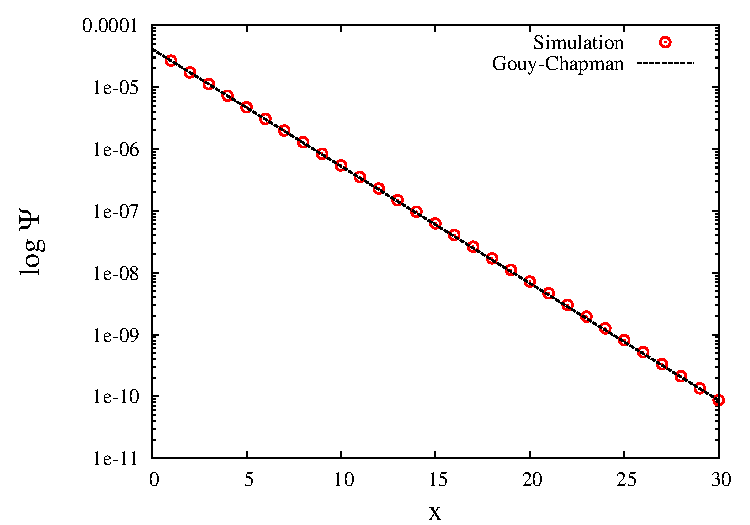
\includegraphics[width=0.495\textwidth]{./pics/test1.pdf}
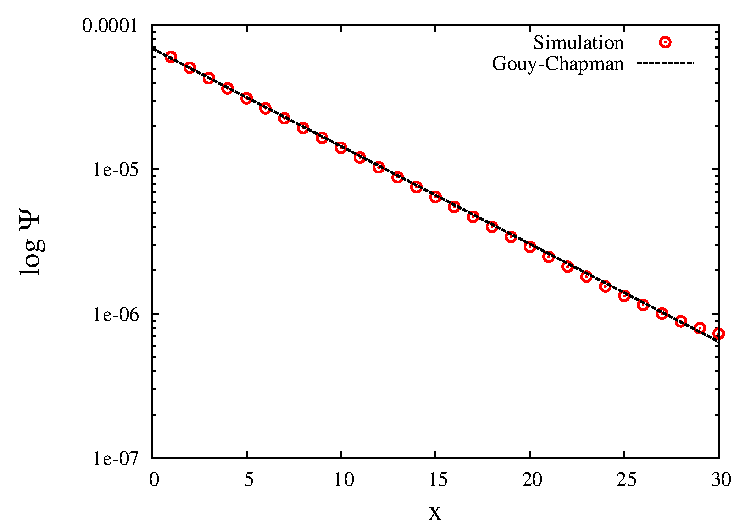
\includegraphics[width=0.495\textwidth]{./pics/test2.pdf}
\caption{Gouy-Chapman theory for electric double layers: The plots compare the simulation results for the electric potential with the analytical solution for $\rho_{0,\pm}=1\e{-2}$ (left) and $\rho_{0,\pm}=1\e{-3}$ (right).} 
\label{fig1} 
\end{figure}


\begin{equation}\label{gouychapman}
\Psi(x) = \Psi_D \exp(-\kappa\, x)
\end{equation}
with $\kappa$ as inverse Debye length 
\begin{equation}
\kappa = l_D^{-1} = \sqrt{8\pi\, l_B \, I}.
\end{equation}
The Bjerrum length $l_B$ is given by 
\begin{equation}
l_B = \frac{\beta\,e^2}{4\pi\,\varepsilon}
\end{equation} 

with $\beta^{-1}=k_B T$, $e$ as unit charge and $\varepsilon=\varepsilon_0\varepsilon_r$ 
as dielectric permittivity.
The parameter 

\begin{equation}
I = \frac{1}{2}\sum_k z_k^2\; \rho_{B,k}
\end{equation} 

is the ionic strength 
of the electrolyte with $z_k$ as valencies of species $k$
($z_\pm=\pm 1$ for simple symmetric electrolyte) and $\rho_{B,k}$ as 
bulk charge density of species $k$ far away from the wall.
The Stern potential $\Psi_D$ at the surface of the wall is related 
to the surface charge $\sigma$ via

\begin{eqnarray}
\Psi_D&=&\frac{2}{\beta \,e} \sinh^{-1}\left(-\sigma\,p\right)\\
\Psi_D&\simeq&\frac{2}{\beta \,e} \ln\left(-\sigma \, p + \sqrt{(\sigma\,p)^2+1}\right)\\
p &=& \frac{1}{\sqrt{8\, \varepsilon\, \beta^{-1} \,\rho_B}}.
\end{eqnarray}

The quantity $\rho_B=\rho_{B,+}=\rho_{B,-}$ is 
the average bulk charge density of the electrolyte.

We solved the Gouy-Chapman problem for a 
system consisting of $L_x \times L_y \times L_z=64\times4\times4$
lattice sites. Periodic boundary conditions were used at all sides 
and a no-flux boundary conditions was set at $L_x=1$ and $L_x=64$.

\begin{figure}[htpb]
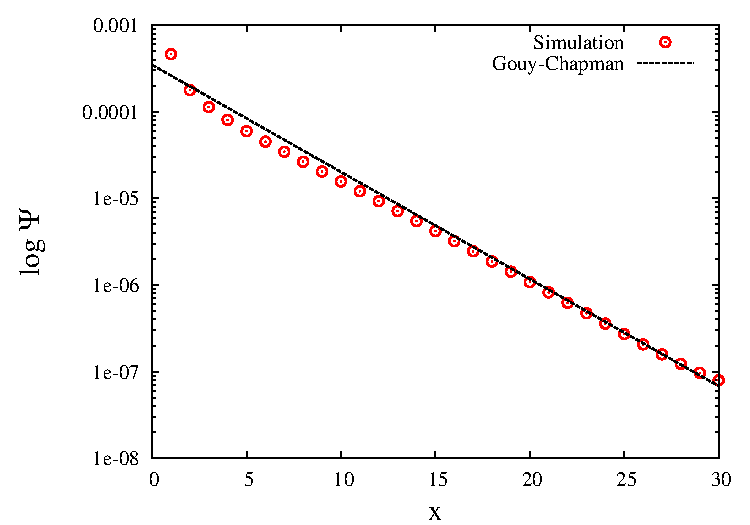
\includegraphics[width=0.495\textwidth]{./pics/test3.pdf}
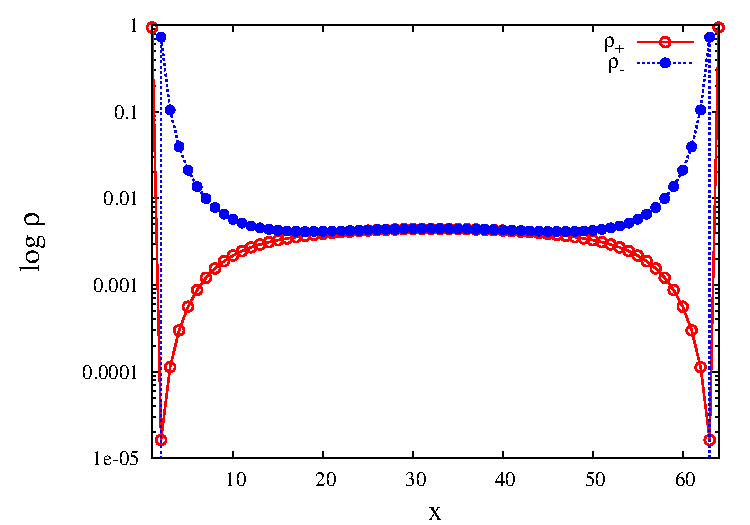
\includegraphics[width=0.495\textwidth]{./pics/test3-rho.pdf}
\caption{Nonlinear regime: For larger surface charges the solution deviates from the low-potential approximation Eq. \ref{gouychapman} to the Gouy-Chapman theory. The righthand picture shows the charge distribution across the gap.} 
\label{fig2} 
\end{figure}

 
The parameters were chosen as follows (all in simulation units):
unit charge $e=1$, temperature $k_B T=\beta^{-1}=3.333\e{-5}$, valency $z_{\pm}=\pm1$, 
dielectric permittivity $\varepsilon=3.3\e{3}$, diffusivities 
of the species $D_{\pm}=1\e{-2}$ and initial densities $\rho_{0,\pm}=1\e{-2}$.
The entire system was electro-neutral and had a Bjerrum length $l_B=0.723$.

At first we tested the linear case applying a small positive surface charge
$\sigma=3.125\e{-2}$, which led to bulk charge density $\rho_{B,+}=\rho_{B,-}=1.044\e{-2}$, 
Debye length $l_D=2.295$ and surface potential $\Psi_D=2.136\e{-5}$.
The potential was initialised with zero and had a value $\Psi_c=-2.364\e{-6}$ 
in the centre of the system after equilibration which we subtracted in the 
following analysis.

We reduced the initial density of the electrolyte to $\rho_{0,\pm}=1\e{-3}$,
which resulted in bulk charge densities  
$\rho_{B,+}=1.298\e{-3}, \rho_{B,-}=1.370\e{-3}$, 
Debye length $l_D=6.420$, surface potential $\Psi_D=5.451\e{-5}$
and centre potential $\Psi_c=-1.256\e{-5}$.
The comparison with the approximate solution Eq. \ref{gouychapman} is shown 
in Fig. \ref{fig1}.

For larger surface charges the low-potential assumption which led to Eq. \ref{gouychapman}
is no longer valid and the nonlinear nature of the Poisson-Boltzmann 
equation becomes evident.
Fig. \ref{fig2} shows the results for a surface charge $\sigma=9.375\e{-1}$
and electrolyte density $\rho_{0,\pm}=3\e{-3}$. We obtained for   
bulk charge densities $\rho_{B,+}=4.443\e{-3}$ and $\rho_{B,-}=4.461\e{-3}$, 
Debye length $l_D=3.514$, the surface potential $\Psi_D=2.267\e{-4}$
and the centre potential $\Psi_c=-3.395\e{-5}$. 

\subsubsection{Liquid-junction potential}

The liquid junction potential 
is a charge separation process that 
occurs when electrolytes with slightly different concentrations
whose species have different diffusivities are brought into contact.
Charges from the regions of higher concentration diffuse   
into the parts with lower concentration. Due to the difference 
in diffusivity they migrate at different speeds, leaving parts of
the system charged. This leads to a build-up of a potential
which balances the diffusive flux.

After the initial build-up phase the potential decreases slowly 
again until the charge concentration has become homogeneous throughout 
the system. Both timescales of emergence and decay of the potential
can be separated by chosing a sufficiently large system size.

This problem allowed us to verify the correct temporal 
behaviour of the Nernst-Planck equation solver by resolving the transient 
dynamics without having to account for advective terms.

\begin{figure}[h!t]
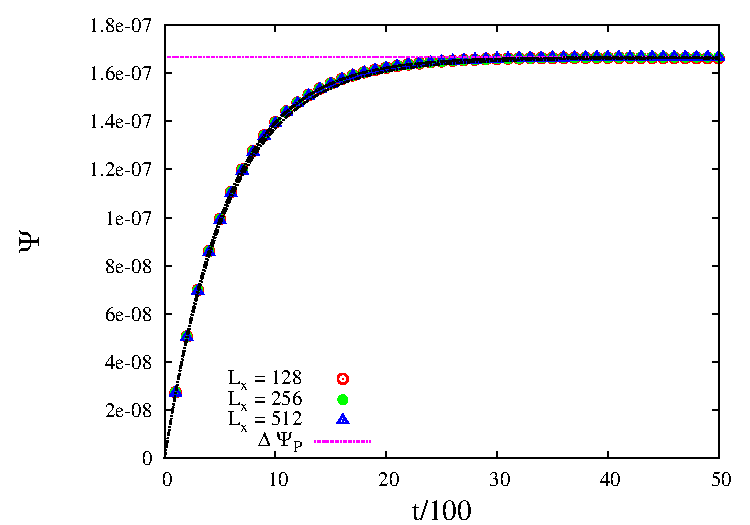
\includegraphics[width=0.495\textwidth]{./pics/test_lj_zoom1.pdf}
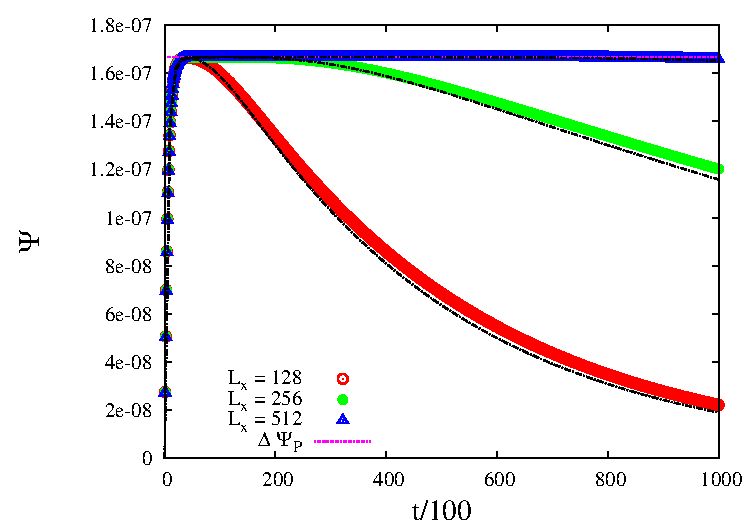
\includegraphics[width=0.495\textwidth]{./pics/test_lj_zoom3.pdf}
\caption{Time evolution of the liquid junction potential for $L_x=128$ (blue), $L_x=256$ (green) and $L_x=512$ (blue). The dashed black curves represent the approximate solution in the limit $l_D/L_x<<1$. Deviations can be seen which are presumably due
to the approximate nature of the analytical solution and the fact that we
have a different asymptotic flux close to the boundary - the theoretical 
analysis assumes no flux at a boundary which is infinitely far away from
the diffusive region.} 
\label{fig3} 
\end{figure}

For simplicity we considered systems of size 
$L_x\times L_y\times Lz=128\times4\times4$ and 
$L_x\times L_y\times Lz=256\times4\times4$ with
periodic boundary conditions at either end.
The two halfs were electroneutral and had ionic concentrations 
$\rho_{L,\pm}=\rho_{0,\pm} + \delta\rho$ and 
$\rho_{R,\pm}=\rho_{0,\pm} - \delta\rho$ 
with $\rho_{0,\pm}=1\e{-2}$ and $\delta\rho = 0.01$.

The potential difference between both sides during the build-up 
obeys approximately

\begin{equation}
\Delta\Psi(t)\simeq\Delta\Psi_P \left\{1-\exp\left(-\frac{t}{\tau_e}\right)\right\}\\
\end{equation}

with 

\begin{equation}
\Delta\Psi_P=\frac{(D_+ D_-)}{\beta e (D_+ + D_-)} \frac{\delta\rho}{\rho_0}\\ 
\end{equation}

as saturation value of the potential difference.
The saturation time scale is given by

\begin{equation}
\tau_e=\frac{\varepsilon}{\beta \, e^2 (D_+ + D_-) \rho_0}.
\end{equation}

\begin{figure}[htpb]
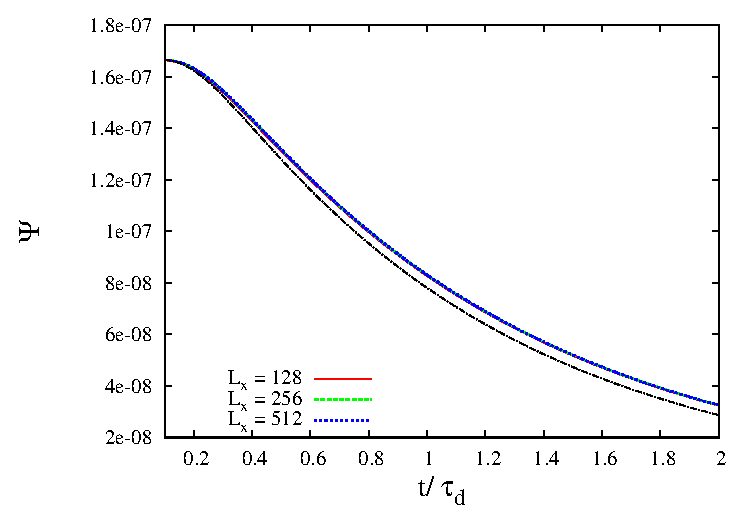
\includegraphics[width=0.9\textwidth]{./pics/test_lj_decay1.pdf}
\caption{Rescaled plot of the decay: Times have been Time evolution of the liquid junction potential for $L_x=128$ (blue), $L_x=256$ (green) and $L_x=512$ (blue). The dashed black curves represent the approximate solution in the limit $l_D/L_x<<1$. Deviations can be seen which are due
to the approximate nature of the analytical solution and the diffusive fluxes close to the boundary.} 
\label{fig4} 
\end{figure}

A more exact solution can be derived in the limit $l_D/L_x<<1, N\to\infty$: 
 
\begin{eqnarray}
\Delta\Psi(t)&=&\Delta\Psi_P \left\{1-\exp\left(-\frac{t}{\tau_e}\right)\right\}\frac{4}{\pi}\left\{\sum_{m=1}^N \frac{\sin^3(m\pi/2)}{m} \exp\left(-\frac{ m^2\, t}{\tau_d}\right)\right\}\\
\tau_d&=&\frac{L^2}{2\pi^2 (D_+ + D_-)}.\label{taud}
\end{eqnarray}

It contains as well the dependence on the decay timescale $\tau_d$.
Only odd indices $m$ contribute to the sum:
 
\begin{eqnarray}
\sum_{m=1}^N \frac{\sin^3(m\pi/2)}{m} \exp\left(-\frac{m^2\, t}{\tau_d}\right)&=&\nonumber\\
&&\hspace*{-4cm} \exp\left(-\frac{t}{\tau_d}\right)-\frac{1}{3} \exp\left(-\frac{9 t}{\tau_d}\right)+\frac{1}{5}\exp\left(-\frac{25t}{\tau_d}\right)-\frac{1}{9}\exp\left(-\frac{81 t}{\tau_d}\right)+\ldots
\end{eqnarray}

A complete discussion of the solution can be found in \cite{Mafe}. 
There, the upper limit of significant modes has been also estimated as $N_{max} = L/\pi l_D$.
Note the factor 2 difference between Eq. \ref{taud} and the corresponding expression in \cite{Mafe}.

The following parameters were used:
dielectric permittivity $\epsilon=3.3\e{3}$, temperature $\beta^{-1}=3.333\e{-5}$, unit charge $e=1$, valency $z_\pm=\pm1$, diffusivities $D_+=0.0125$ and $D_-=0.0075$.
We obtained
$\Delta\Psi_P=1.6667\e{-7}$, $\tau_e=550$, $\tau_d=41501.2\, (L_x=128)$, $\tau_d=166004.6\, (L_x=256)$ and $\tau_d=664018.5 (L_x=512)$.
The results for the potential difference over time are shown in Fig. \ref{fig3}.

Fig. \ref{fig4} shows results with times rescaled to the decay 
time scale $\tau_d$ (cf. Eq. \ref{taud}). Obviously the 
deviations we observe are not due to the limited system size 
and have a more systematic origin. 

The curves coincide if 
the theoretic limit for $\tau_d$ is rescaled by a factor $1.067$,
suggesting the effective system length for this sort of setup is
actually about 3\% larger than the numerical value.

A reason for this might be the approximate nature of the analytical solution 
and the fact that it was gained
for an infinitely large system with constant charge concentrations,
vanishing currents at both ends and finite diffusive zone of size $L_x$.
In our situation the entire system is within the diffusive zone.
This may lead to smaller effective diffusivities or larger effective
system sizes.
Interestingly, all runs with solid walls at both ends resulted in 
oscillatory behaviour and an effective system size of $2L_x$.


\subsubsection{Electroosmotic Flow}

To test the implementation with all couplings to external and 
internal forces we consider a forced charged fluid in a slit
of size $L_z$. An electrostatic field $E_{||}$ is allied
parallel to the walls. The entire system is electroneutral with 
each wall having the surface charge density $\sigma$ 
and compensationg counterions with total charge $2 \sigma A_{wall}$
in the fluid.

In equilibrium the charge density at a distance $x$ from the wall obeys

\begin{equation}
\rho(x)=\frac{\rho_0}{\cos^2(K\,x)}
\end{equation}

with 

\begin{equation}
\rho_0=K^2/2\pi l_B
\end{equation}

and 

\begin{eqnarray}
K \,L_x \tan\left(\frac{K\, L_x}{2}\right)&=&\pi\, l_B\, L_x\, 2\sigma\label{kex} \\
K \,L_x&\simeq&\sqrt{4\pi \,l_B\,L_x\,2\sigma}\label{klin}.
\end{eqnarray}


The liniarised version Eq. \ref{klin} has only a limited range of applicabilty.
We solved Eq. \ref{kex} numerically and found solutions 
$K=0.01959\; (\sigma=0.003125)$ and $K=0.03311\; (\sigma=0.00125)$, 
which is reasonably far away from the 
theoretical limit $K_{max}=\pi/L_x$ set by the tangent. 

Note the factor 2 difference on the lhs of Eq. \ref{kex} with respect 
to \cite{Capuani, Rotenberg}. There is also a factor $L_x$ missing on 
the rhs of Eq. \ref{klin}.

The steady state velocity of the fluid can be derived from the 
force balance of the gradient of the stresses and the electrostatic
forces:

\begin{eqnarray}
v_y(x)&=&\hat{v} \ln\left(\frac{\cos(K\,x)}{\cos(K\,L_x/2)}\right)\label{vy}\\
\hat{v}&=&\frac{e \,E_{||}\rho_o}{\eta\, K^2}=\frac{e \,E_{||}}{2\pi\eta l_B}\label{vhat}
\end{eqnarray}

The result for two different charge densities is shown in Fig. \ref{fig6}.
The accuracy is acceptable with deviations for high surface 
charged potentially being caused by the chosen discretisation or 
by the numerical solution of Eq. \ref{kex} approaching the limit 
of $\pi/L_z\simeq0.049$.  

\begin{figure}[htpb]
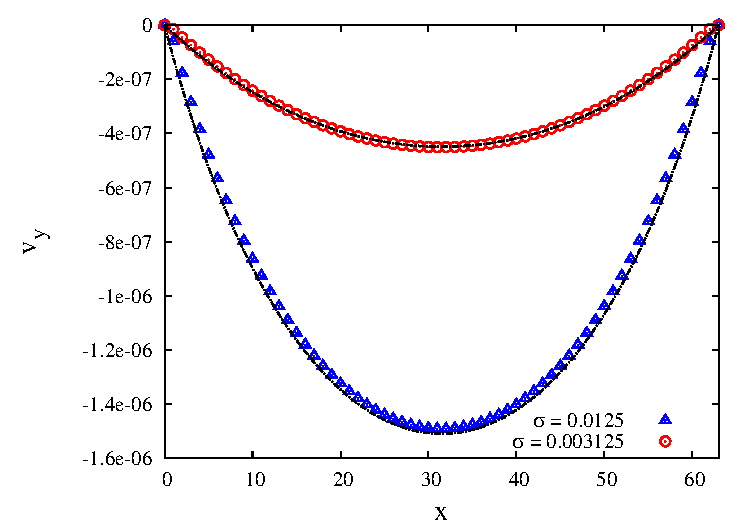
\includegraphics[width=0.9\textwidth]{./pics/test_eo.pdf}
\caption{Steady state flow profile across a slit of width $L_x=63$ for an applied field of magnitude $e \beta E L_x=1.89$ for two different charge densities $\sigma=0.003125$ (red) and $\sigma=0.0125$ (blue), Bjerrum length $l_B=0.7234$, viscosity $\eta=0.1$ and unit charge $e=1$. The dashed black lines correspond to theoretical prediction according to Eqs. \ref{vy} and \ref{vhat}.} 
\label{fig6} 
\end{figure}

\subsubsection{Debye-H\"uckel Theory}

We have tested the implementation for a single fixed
colloid and compared the result with Debye-H\"uckel theory. A result
is shown in Fig.~\ref{fig7}.
We used the following parametrisation:

$L_x \times L_y \times L_z=64\times64\times64$,
$D_+=D_-=0.01$,
$e=1$, 
$z_{\pm}=1$,
$\beta^{-1}=3.333\e{-5}$,
$\varepsilon=3.3\e{3}$,
$l_B=0.723$.

For a central and fixed colloid of radius $R_c=7.5$ carrying a positive unit charge
$q_{c,+}=1.0, q_{c,-}=0$ we obtained 
$\rho_{c,+}=5.58\e{-4}$,
$\rho_{el}=\rho_{B,\pm}=1\e{-2}$, 
$\Psi_D=8.836\e{-7}$ for $2\,R_c=16$.

For a higher larger positive charge $q_{c,+}=4.0$ we got
$\rho_{c,+}=2.23\e{-3}$
$\rho_{el}=\rho_{B,\pm}=5\e{-3}$ 
$\Psi_D=4.993\e{-6}$ for $2\,R_c=16$.

\begin{figure}[htpb]
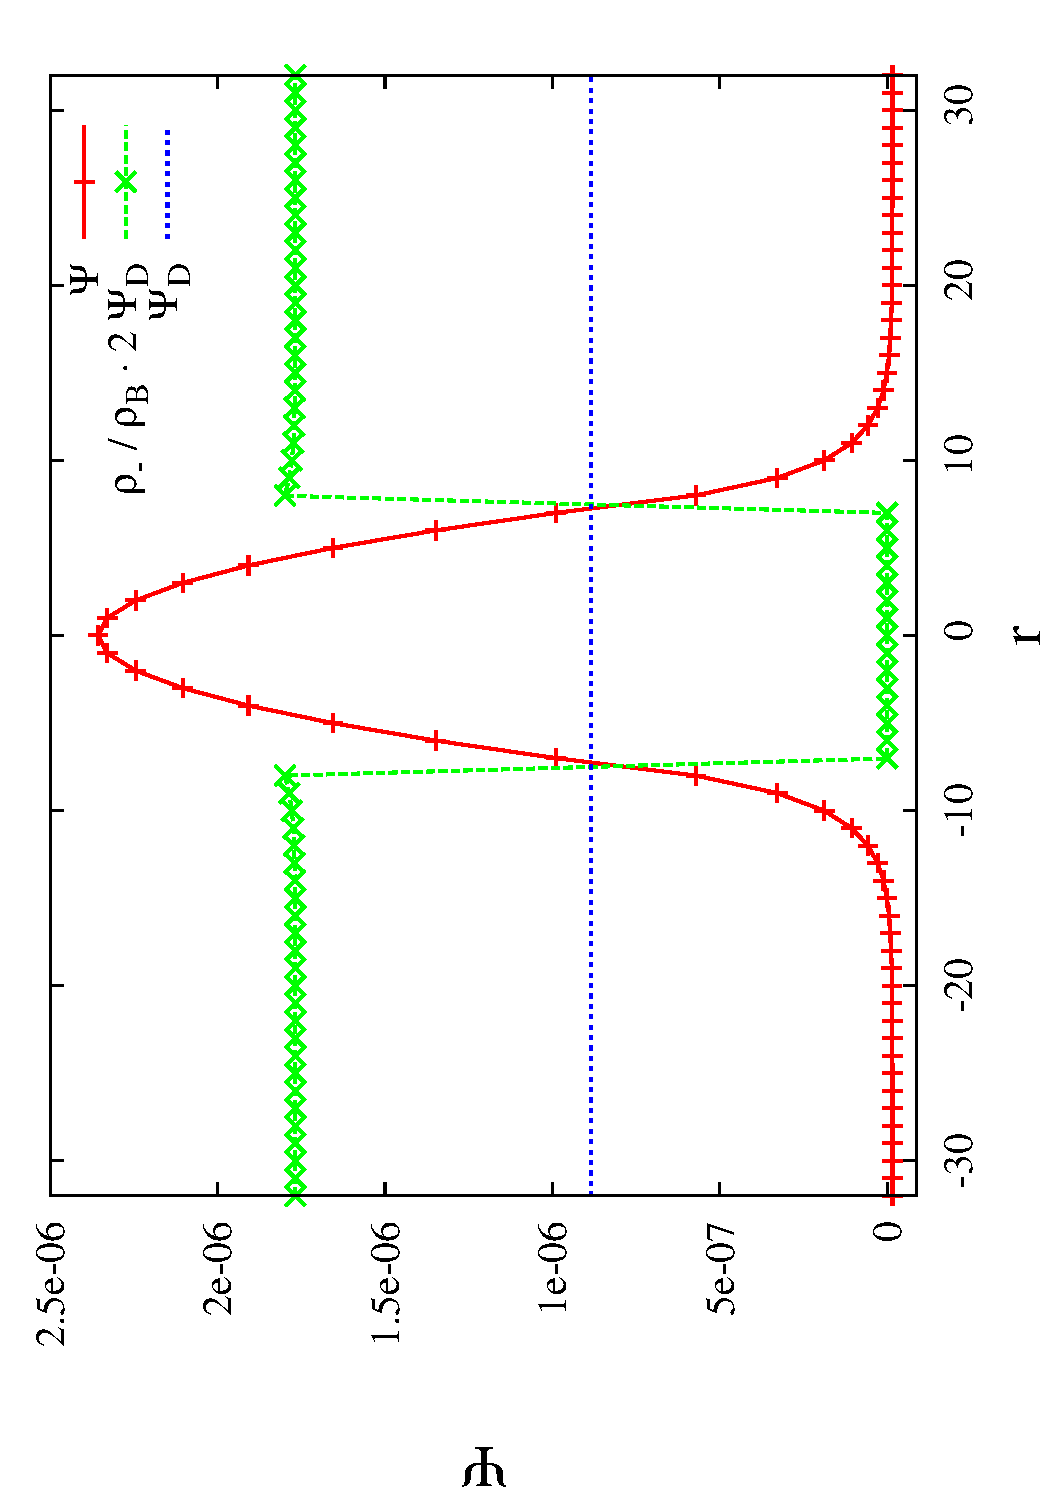
\includegraphics[angle=-90,width=0.9\textwidth]{./pics/test_dh1.pdf}\\
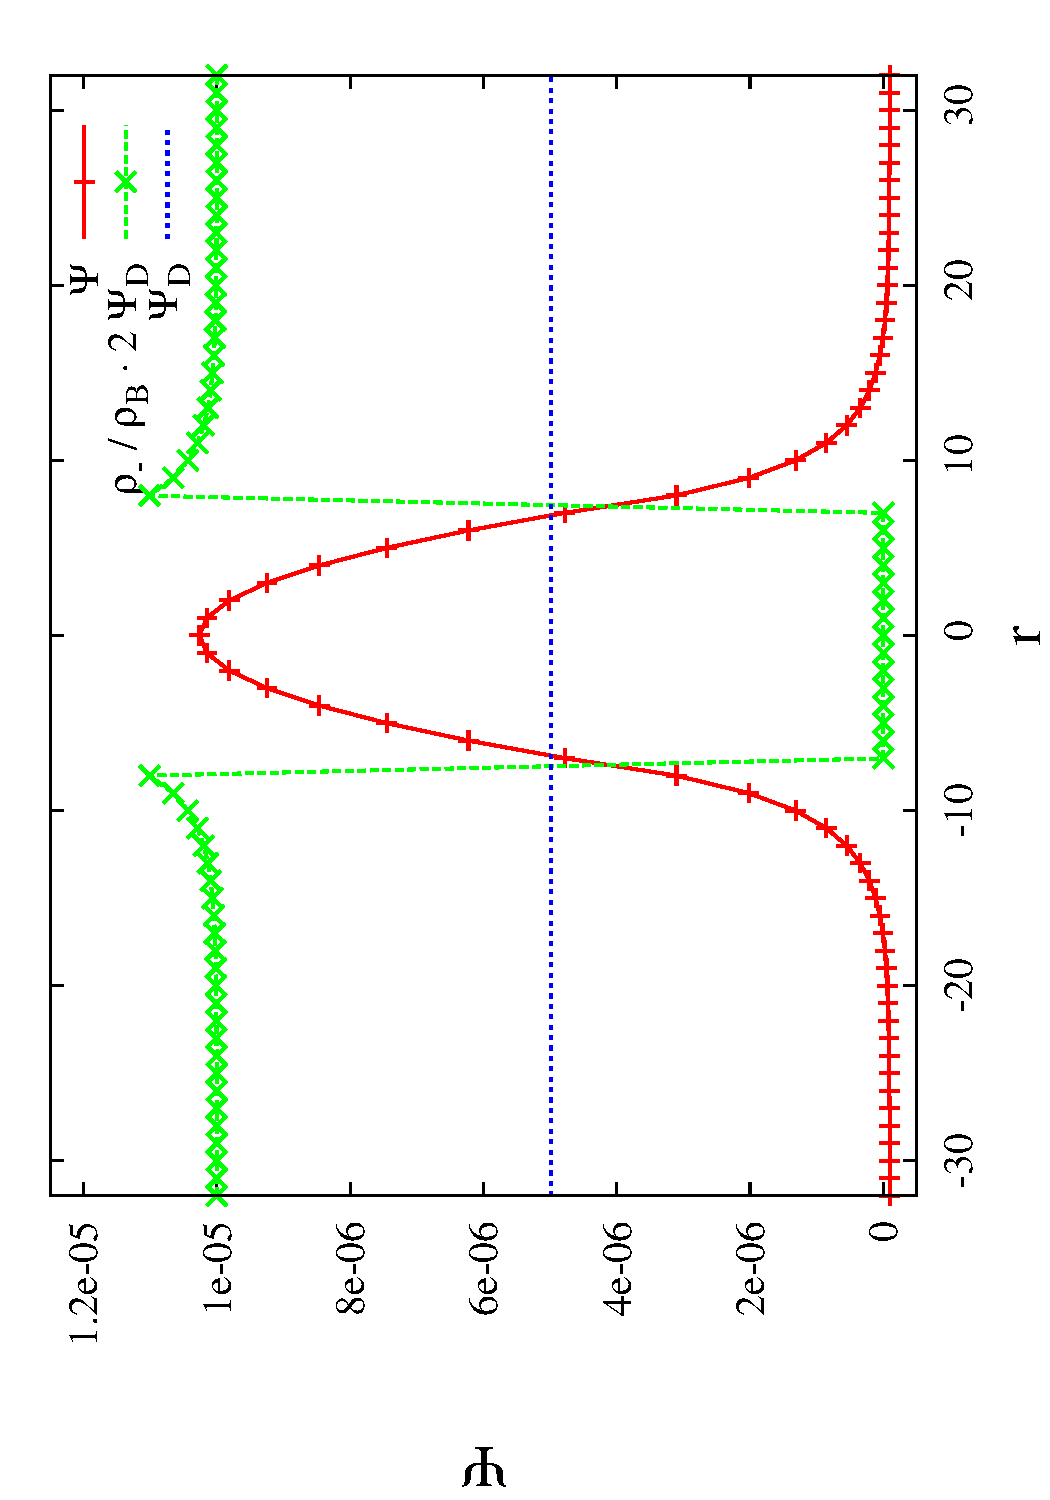
\includegraphics[angle=-90,width=0.9\textwidth]{./pics/test_dh2.pdf}
\caption{Debye-H\"uckel theory for positively charged colloid: the picture
shows a cut through the center of a single colloid in a peridoic system.
The potential is shown in red, the Stern potential in blue, and the negative 
charge density in green. The colloid is in the center.}
\label{fig7}
\end{figure}
\clearpage

\subsubsection{Scaling of the SOR}

We have run some simple scaling tests for the electrokinetic problem
with zero fluid velocity. A system of $128^3$ lattice sites was used
as representative of a small production system. The code was run on
the Mare Nostrum machine in Barcelona for a small number of time
steps to assess performance on up to 512 MPI tasks. The results are
shown in Fig. \ref{fig5}. 

While the scaling for the Nernst Planck part of
the calulcation are reasonable, it can be seen that the SOR routine
used to solve the Poisson equation is not really acceptable. This
was not unexpected. Some improvements might be possible, but the
algorithm is essentailly unsuitable for large systems. 

\begin{figure}[htpb]
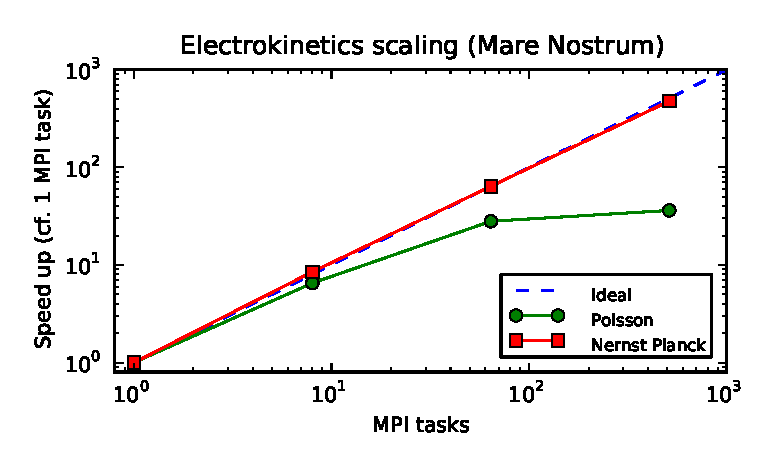
\includegraphics[width=0.9\textwidth]{./pics/scaling.pdf}
\caption{Scaling of a system of $128^3$ lattice sites on up to 512 MPI tasks. 
While the scaling for the Nernst Planck part of the calulcation are reasonable, 
it can be seen that the SOR routine used to solve the Poisson equation deviates
strongly from ideal behaviour.} 
\label{fig5} 
\end{figure}

\subsubsection{Scaling with Krylov Subspace Solver}

We use a Krylov subspace solver from the Portable Extendabl Toolkit for Scientific Computation (PETSc. 

\begin{figure}[htpb]
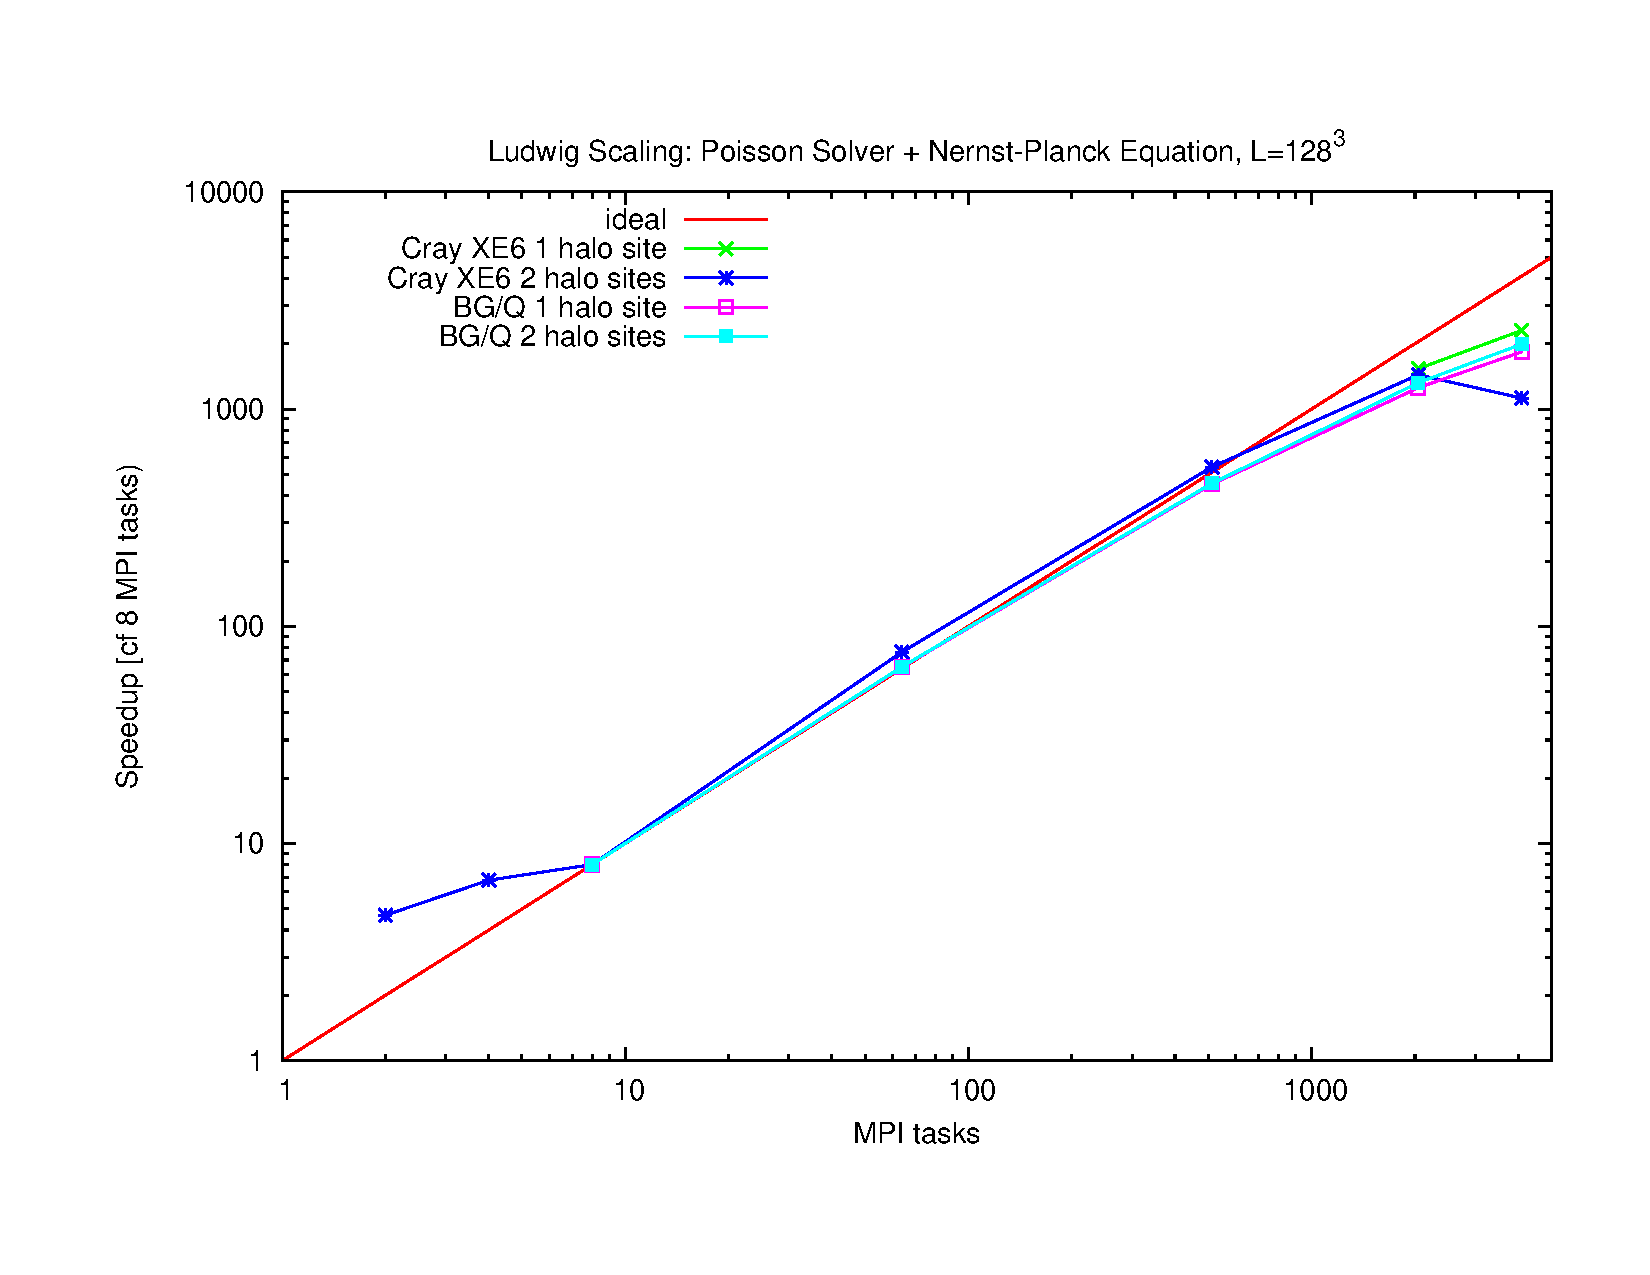
\includegraphics[width=0.9\textwidth]{./pics/petsc_scaling.pdf}
\caption{Scaling of a system of $128^3$ lattice sites on up to 4096 MPI tasks. 
The scaling of both the Nernst Planck part as well as the Poisson solver are only limited by the overhead of communication to computation at very small decompositions.} 
\label{fig6} 
\end{figure}
\clearpage


\subsection{User input}

%%%%%%%%%%%%%%%%%%%%%%%%%%%%%%%%%%%%%%%%%%%%%%%%%%%%%%%%%%%%%%%%%%%%%%%%%%%%%%
%
%  input.tex
%
%  Instructions for contents of the user input file.
%
%  Edinburgh Soft Matter and Statistical Physics Group and
%  Edinburgh Parallel Computing Centre
%
%  (c) 2016-2017 The University of Edinburgh
%
%%%%%%%%%%%%%%%%%%%%%%%%%%%%%%%%%%%%%%%%%%%%%%%%%%%%%%%%%%%%%%%%%%%%%%%%%%%%%%

\section{The Input File}

\subsection{General}

By default, the run time expects to find user input in a file
\texttt{input} in the current working directory. If a different
file name is required, its name
should be provided as the sole command line argument, e.g.,
\begin{lstlisting}
./Ludwig.exe input_file_name
\end{lstlisting}
If the input file is not located in the current working directory
the code will terminate immediately with an error message.

When an input file is located, its content is read by a single MPI
task, and its contents then broadcast to all MPI relevant tasks.
The format of the file is plain ASCII text, and its contents are
parsed on a line by line basis. Lines may contain the following:
\begin{itemize}
\item comments introduced by \texttt{\#}.
\item key value pairs separated by white space.
\end{itemize}
Blank lines are treated as comments. The behaviour of the code is
determined by a set of key value pairs. Any given key may appear
only once in the input file; unused key value pairs are not reported.
If the key value pairs are not correctly formed, the code will terminate
with an error message and indicate the offending input line.

Key value pairs may be present in the input file, but have no effect for
any given run: they are merely ignored. Relevant control parameters for
given input are reported in the standard output.

\subsubsection{Key value pairs}

Key value pairs are made up of a key --- an alphanumeric string with no
white space --- and corresponding value following white space. Values
may take on the follow forms:
\begin{lstlisting}
key_string           value_string

key_integer_scalar  1
key_integer_vector  1_2_3

key_double_scalar    1.0
key_double_vector    1.0_2.0_3.0
\end{lstlisting}
Values which are strings should contain no white space. Scalar parameters
may be integer values, or floating point values with a decimal point
(scientific notation is also allowed).  Vector parameters are introduced
by a set of three values (to be interpreted as $x,y,z$ components of the
vector in Cartesian coordinates) separated by an underscore. The identity
of the key will specify what type of value is expected. Keys and (string)
values are case sensitive.


Most keys have an associated default value which will be used if
the key is not present. Some keys must be specified: an error will
occur if they are missing. The remainder of this part
of the guide details the various choices for key value pairs,
along with any default values, and any relevant constraints.

\subsection{The Free Energy}
\label{input-free-energy}

The choice of free energy is determined as follows:
\begin{lstlisting}
free_energy   none
\end{lstlisting}
The default value is \texttt{none}, i.e., a simple Newtonian fluid is used.
Possible values of the \texttt{free\_energy} key are:
\begin{lstlisting}
#  none                     Newtonian fluid [DEFAULT]
#  symmetric                Symmetric binary fluid (finite difference)
#  symmetric_lb             Symmetric binary fluid (two distributions)
#  brazovskii               Brazovskii smectics
#  surfactant               Surfactants
#  polar_active             Polar active gels
#  lc_blue_phase            Liquid crystal (nematics, cholesterics, BPs)
#  lc_droplet               Liquid crystal emulsions
#  fe_electro               Single fluid electrokinetics
#  fe_electro_symmetric     Binary fluid electrokinetics
\end{lstlisting}

The choice of free energy will control automatically a number of factors
related to choice of order parameter, the degree of parallel communication
required, and so on. Each free energy has a number of associated parameters
discussed in the following sections.

Details of general (Newtonian) fluid parameters, such as viscosity,
are discussed in Section~\ref{input-fluid-parameters}.

\subsubsection{Symmetric Binary Fluids}

We recall that the free energy density is, as a function of compositional
order $\phi$:
\[
{\textstyle \frac{1}{2}} A\phi^2 +
{\textstyle \frac{1}{4}} B\phi^4 +
{\textstyle \frac{1}{2}} \kappa (\mathbf{\nabla}\phi)^2.
\]

Parameters are introduced by (with default values):
\begin{lstlisting}
free_energy  symmetric
A            -0.0625                         # Default: -0.003125
B            +0.0625                         # Default: +0.003125
K            +0.04                           # Default: +0.002
\end{lstlisting}
Common usage has $A < 0$ and $B = -A$ so that $\phi^\star = \pm 1$.
The parameter $\kappa$
(key \texttt{K}) controls
the interfacial energy penalty and is usually positive.

\subsubsection{Brazovskii smectics}
\label{input-brazovskki-smectics}
The free energy density is:
\[
{\textstyle \frac{1}{2}} A\phi^2 +
{\textstyle \frac{1}{4}} B\phi^4 +
{\textstyle \frac{1}{2}} \kappa (\mathbf{\nabla}\phi)^2 +
{\textstyle \frac{1}{2}} C (\nabla^2 \phi)^2 
\]

Parameters are introduced via the keys:
\begin{lstlisting}
free_energy  brazovskii
A             -0.0005                        # Default: 0.0
B             +0.0005                        # Default: 0.0
K             -0.0006                        # Default: 0.0
C             +0.00076                       # Default: 0.0
\end{lstlisting}
For $A<0$, phase separation occurs with a result depending on $\kappa$:
one gets two symmetric phases for $\kappa >0$ (cf.\ the symmetric case)
or a lamellar phase for $\kappa < 0$. Typically, $B = -A$ and the
parameter in the highest derivative $C > 0$.

\subsubsection{Surfactants}
\label{input-surfactants}

The surfactant free energy should not be used at the present time.

\subsubsection{Polar active gels}
\label{input-polar-active-gels}

The free energy density is a function of vector order parameter $P_\alpha$:
\[
{\textstyle \frac{1}{2}} A P_\alpha P_\alpha +
{\textstyle \frac{1}{4}} B (P_\alpha P_\alpha)^2 +
{\textstyle \frac{1}{2}} \kappa (\partial_\alpha P_\beta)^2
\]

There are no default parameters:
\begin{lstlisting}
free_energy        polar_active
polar_active_a    -0.1                       # Default: 0.0
polar_active_b    +0.1                       # Default: 0.0
polar_active_k     0.01                      # Default: 0.0
\end{lstlisting}
It is usual to choose $B > 0$, in which case $A > 0$ gives
an isotropic phase, whereas $A < 0$ gives a polar nematic phase.
The elastic constant $\kappa$ (key \texttt{polar\_active\_k})
is positive.

\subsubsection{Liquid crystal}
\label{input-liquid-crystal}
The free energy density is a function of tensor order parameter
$Q_{\alpha\beta}$:
\begin{eqnarray}
{\textstyle\frac{1}{2}} A_0 (1 - \gamma/3)Q^2_{\alpha\beta} -
{\textstyle\frac{1}{3}} A_0 \gamma
                        Q_{\alpha\beta}Q_{\beta\delta}Q_{\delta\alpha} +
{\textstyle\frac{1}{4}} A_0 \gamma (Q^2_{\alpha\beta})^2
\nonumber \\
+ {\textstyle\frac{1}{2}} \Big(
\kappa_0 (\epsilon_{\alpha\delta\sigma} \partial_\delta Q_{\sigma\beta} +
2q_0 Q_{\alpha\beta})^2 + \kappa_1(\partial_\alpha Q_{\alpha\beta})^2 \Big)
\nonumber
\end{eqnarray}

The corresponding \texttt{free\_energy} value, despite its name, is
suitable for nematics and cholesterics, and not just blue phases:
\begin{lstlisting}
free_energy      lc_blue_phase
lc_a0            0.01                       # Deafult: 0.0
lc_gamma         3.0                        # Default: 0.0
lc_q0            0.19635                    # Default: 0.0
lc_kappa0        0.00648456                 # Default: 0.0
lc_kappa1        0.00648456                 # Default: 0.0
\end{lstlisting}
The bulk free energy parameter $A_0$ is positive and controls the
energy scale (key \texttt{lc\_a0}); $\gamma$ is positive and
influences the position in the phase diagram relative to the
isotropic/nematic transition (key \texttt{lc\_gamma}).
The two elastic constants must be equal, i.e., we enforce the
single elastic constant approximation (both keys \texttt{lc\_kappa0} and
\texttt{lc\_kappa1} must be specified).

Other important parameters in the liquid crystal picture are:
\begin{lstlisting}
lc_xi            0.7                         # Default: 0.0
lc_Gamma         0.5                         # Default: 0.0
lc_active_zeta   0.0                         # Default: 0.0
\end{lstlisting}
The first is $\xi$ (key \texttt{lc\_xi}) is the effective molecular
aspect ratio and should be in the range $0< \xi< 1$. The rotational
diffusion constant is $\Gamma$ (key \texttt{lc\_Gamma}; not to be
confused with \texttt{lc\_gamma}). The (optional) apolar activity
parameter is $\zeta$ (key \texttt{lc\_active\_zeta}).

\subsubsection{Liquid crystal anchoring}

Different types of anchoring are available at solid surfaces, with
one or two related free energy parameters depending on the type.
The type of anchoring may be set independently for stationary
boundaries (walls) and colloids.
\begin{lstlisting}
lc_anchoring_strength     0.01               # free energy parameter w1
lc_anchoring_strength_2   0.0                # free energy parameter w2
lc_wall_anchoring         normal             # ``normal'' or ``planar''
lc_coll_anchoring         normal             # ``normal'' or ``planar''
\end{lstlisting}
See section \ref{section-lc-anchoring} for details of surface anchoring.

\subsubsection{Liquid crystal emulsion}
\label{input-liquid-crystal-emulsion}

This an interaction free energy which combines the symmetric and liquid
crystal free energies. The liquid crystal free energy constant $\gamma$
becomes a
function of composition via $\gamma(\phi) = \gamma_0 + \delta(1 + \phi)$,
and a coupling term is added to the free energy density:
\[
WQ_{\alpha\beta} \partial_\alpha \phi \partial_\beta \phi.
\]
Typically, we might choose $\gamma_0$ and $\delta$ so that
$\gamma(-\phi^\star) < 2.7$ and the $-\phi^\star$ phase is isotropic,
while $\gamma(+\phi^\star) > 2.7$ and the
$+\phi^\star$ phase is ordered (nematic, cholesteric, or blue phase).
Experience suggests that a suitable choice is $\gamma_0 = 2.5$ and
$\delta = 0.25$.

For anchoring constant $W > 0$, the liquid crystal anchoring at the
interface is planar, while for $W < 0$ the anchoring is normal. This
is set via key \texttt{lc\_droplet\_W}.

Relevant keys (with default values) are:
\begin{lstlisting}
free_energy            lc_droplet

A                      -0.0625
B                      +0.0625
K                      +0.053

lc_a0                   0.1
lc_q0                   0.19635
lc_kappa0               0.007
lc_kappa1               0.007

lc_droplet_gamma        2.586                # Default: 0.0
lc_droplet_delta        0.25                 # Default: 0.0
lc_droplet_W           -0.05                 # Default: 0.0
\end{lstlisting}
Note that key \texttt{lc\_gamma} is not set in this case.

\subsection{System Parameters}
\label{input-system-parameters}

Basic parameters controlling the number of time steps
and the system size are:
\begin{lstlisting}
N_start      0                              # Default: 0
N_cycles     100                            # Default: 0
size         128_128_1                      # Default: 64_64_64
\end{lstlisting}
A typical simulation will start from time zero (key \texttt{N\_start})
and run for a certain number of time steps (key \texttt{N\_cycles}).
The system size (key \texttt{size}) specifies the total number of
lattice sites in each dimension. If a two-dimensional system is
required, the extent in the $z$-direction must be set to unity, as
in the above example.

If a restart from a previous run is required, the choice of parameters
may be as follows:
\begin{lstlisting}
N_start      100
N_cycles     400
\end{lstlisting}
This will restart from data previously saved at time step 100, and
run a further 400 cycles, i.e., to time step 500.
% TODO Cross-reference to I/O.

\subsubsection{Parallel decomposition}

In parallel, the domain decomposition is closely related to the
system size, and is specified as follows:
\begin{lstlisting}
size         64_64_64
grid         4_2_1
\end{lstlisting}
The \texttt{grid} key specifies the number of MPI tasks required in
each coordinate direction. In the above example, the decomposition
is into 4 in the $x$-direction, into 2 in the $y$-direction, while
the $z$-direction is not decomposed. In this example, the local domain
size per MPI
task would then be $16\times32\times64$. The total number of MPI tasks
available must match the total implied by \texttt{grid} (8 in the
example).

The \texttt{grid} specifications must exactly divide the system size;
if no decomposition is possible, the code will terminate with an error
message.
If the requested decomposition is not valid, or \texttt{grid} is
omitted, the code will try to supply a decomposition based on
the number of MPI tasks available and \texttt{MPI\_Dims\_create()};
this may be implementation dependent.


\subsection{Fluid Parameters}
\label{input-fluid-parameters}

Control parameters for a Newtonian fluid include:
\begin{lstlisting}
fluid_rho0                 1.0
viscosity                  0.166666666666666
viscosity_bulk             0.166666666666666
isothermal_fluctuations    off
temperature                0.0
\end{lstlisting}
The mean fluid density is $\rho_0$ (key \texttt{fluid\_rho0}) which
defaults to unity in lattice units; it is not usually necessary to
change this. The shear viscosity is
\texttt{viscosity} and as default value 1/6 to correspond to
unit relaxation time in the lattice Boltzmann picture. Reasonable
values of the shear viscosity are $0.2 > \eta > 0.0001$ in lattice
units. Higher values move further into the over-relaxation region, and can
result in poor behaviour. Lower
values increase the Reynolds number and tend to cause
problems with stability. The bulk
viscosity has a default value which is equal to whatever shear
viscosity has been selected. Higher values of the bulk viscosity
may be set independently and can help to suppress large deviations
from incompressibility and maintain numerical stability
in certain situations.

If fluctuating hydrodynamics is wanted, set the value of
 \texttt{isothermal\_fluctuations} to \texttt{on}. The associated
temperature is in lattice units: reasonable values (at $\rho_0 = 1$)
are $0 < kT < 0.0001$. If the temperature is too high, local
velocities will rapidly exceed the Mach number constraint and
the simulation will be unstable.

\subsection{Lees Edwards Planes}

Constant uniform shear may be introduced via a number of Lees Edwards
planes with given speed. This is appropriate for fluid-only
systems with periodic boundaries.
\begin{lstlisting}
N_LE_plane               2           # Number of planes (default: 0)
LE_plane_vel             0.05        # Constant plane speed
\end{lstlisting}
The placing of the planes in the system is as follows.
The number of planes $N$ must
divide evenly the lattice size in the $x$-direction to give an integer
$\delta x$. Planes are then placed at $\delta x / 2, 3\delta x/2, \ldots$.
All planes have the same, constant, velocity jump associated with them:
this is positive in the positive $x$-direction. (This jump is usually
referred to as the plane speed.) The uniform shear rate
will be $\dot{\gamma} = N U_{LE} / L_x$ where $U_{LE}$ is the plane
speed (which is always in the $y$-direction).

The velocity gradient or shear direction is $x$, the flow
direction is $y$ and the vorticity direction is $z$.

The spacing between planes must not be less than twice the halo size
in lattice units; 8--16 lattice units may be the practical limit in
many cases. In additional, the speed of the planes must not cause a
violation of the
Mach number constraint in the fluid velocity on the lattice, which
will match the plane speed in magnitude directly either side of the
planes. A value of around 0.05 should be regarded as a maximum safe
limit for practical purposes.

Additional keys associated with the Lees Edwards planes are:
\begin{lstlisting}
LE_init_profile          1           # Initialise u(x) (off/on)
LE_time_offset           10000       # Offset time (default 0)
\end{lstlisting}
If \texttt{LE\_init\_profile} is set, the fluid velocity is initialised
to reflect a steady state shear flow appropriate for the number of
planes at the given speed (ie., shear rate). If set to zero (the default),
the fluid is initialised with zero velocity.

The code works out the current displacement of the planes by computing
$U_{LE} t$, where $t$ is the current time step. A shear run should then
start from $t = 0$, i.e. zero plane displacement.
It is often convenient to run an equilibration with no shear, and
then to start an experiment after some number of steps. This
key allows you to offset the start of the Lees-Edwards motion.
It should then take the value of the start time (in time steps)
corresponding to the restart at the end of the equilibration
period.

There are a couple of additional constraints to use the Lees-Edwards
planes in parallel. In particular, the planes cannot fall at a
processor boundary in the $x$-direction. This means you should
arrange an integer number of planes per process in the $x$-direction.
(For example, use one plane per process; this will also ensure the number
of planes
still evenly divides the total system size.)
This will interleave the planes with the processor decomposition.
The $y$-direction and $z$-direction may be decomposed without
further constraint.

Note that this means a simulation with one plane will only work
if there is one process in the $x$ decomposition.



\subsection{Colloids}
If no relevant key words are present, no colloids will be
expected at run time. The simulation will progress in the
usual fashion with fluid only.

If colloids are required, the \texttt{colloid\_init}
key word must be present to allow the code to determine where
colloid information will come from. The options for the
\texttt{colloid\_init} key word are summarised below:
\begin{lstlisting}
colloid_init             none

#  none                  no colloids [DEFAULT]
#  input_one             one colloid from input file
#  input_two             two colloids from input file
#  input_three           three colloids from input file
#  input_random          Small number at random
#  from_file             Read a separate file (including all restarts)
\end{lstlisting}

For idealised simulations which require 1, 2, or 3 colloids, relevant
initial state information 
for each particle can be included in the input file. In principle, most
of the colloid state as defined in the colloid
state structure in \texttt{colloid.h} may be specified. (Some state is
reserved for internal use only and cannot be set from the input file.)
Furthermore, not all the state is relevant in all simulations ---
quantities such as charge and wetting parameters may not be required,
in which case they a simply ignored.

A minimal initialisation is shown in the following example:
\begin{lstlisting}
colloid_init              input_one

colloid_one_a0            1.25
colloid_one_ah            1.25
colloid_one_r             12.0_12.0_12.0
\end{lstlisting}
This initialises a single colloid with an input radius $a_0=1.25$,
and a hydrodynamic radius $a_h=1.25$; in general both are required,
but they do not have to be equal.
A valid position is required within the extent of the system
$0.5 < x,y,z < L + 0.5$ as specified by the \texttt{size} key word.
State which is not explicitly defined is initialised to zero.

\subsubsection{General Initialisation}

A full list of colloid state-related key words is as follows. All
the quantities are floating point numbers unless explicitly stated
to be otherwise:
\begin{lstlisting}
# colloid_one_nbonds      (integer) number of bonds
#   colloid_one_bond1     (integer) index of bond partner 1
#   colloid_one_bond2     (integer) index of bond partner 2
# colloid_one_isfixedr    colloid has fixed position (integer 0 or 1)
# colloid_one_isfixedv    colloid has fixed velocity (integer 0 or 1)
# colloid_one_isfixedw    colloid has fixed angular velocity (0 or 1)
# colloid_one_isfixeds    colloid has fixed spin (0 or 1)
# colloid_one_type        ``default'' COLLOID_TYPE_DEFAULT
#                         ``active''  COLLOID_TYPE_ACTIVE
#                         ``subgrid'' COLLOID_TYPE_SUBGRID
# colloid_one_a0          input radius
# colloid_one_ah          hydrodynamic radius
# colloid_one_r           position vector
# colloid_one_v           velocity (vector)
# colloid_one_w           angular velocity (vector)
# colloid_one_s           spin (unit vector)
# colloid_one_m           direction of motion (unit) vector for swimmers 
\end{lstlisting}

Note that for magnetic particles, the appropriate initialisation involves
the spin key word \texttt{colloid\_one\_s} which relates to the dipole
moment $\mu \mathbf{s}_i$, while \texttt{colloid\_one\_m} relates to the
direction of motion vector. Do not confuse the two.
It is possible in principle to have magnetic active particles,
in which case the dipole direction or spin ($\mathbf{s}_i$) and the
direction of swimming motion $\mathbf{m}_i$ are allowed to be distinct. 

\begin{lstlisting}
# colloid_one_b1          Squirmer parameter B_1
# colloid_one_b2          Squirmer parameter B_2
# colloid_one_rng         (integer) random number generator state
# colloid_one_q0          charge (charge species 0)
# colloid_one_q1          charge (charge species 1)
# colloid_one_epsilon     Permeativity
# colloid_one_c           Wetting parameter C
# colloid_one_h           Wetting parameter H
\end{lstlisting}

{\bf Example}: Single active (squirmer) particle

The following example shows a single active particle with initial
swimming direction along the $x$-axis.
\begin{lstlisting}
colloid_init              input_one

colloid_one_type          active
colloid_one_a0            7.25
colloid_one_ah            7.25
colloid_one_r             32.0_32.0_32.0
colloid_one_v             0.0_0.0_0.0
colloid_one_m             1.0_0.0_0.0
colloid_one_b1            0.05
colloid_one_b2            0.05
\end{lstlisting}



\subsubsection{Random initialisation}

For suspensions with more than few colloids, but still at
relatively low volume fraction (10--20\% by volume), it is
possible to request initialisation at random positions.

The additional key word value pair \texttt{colloid\_random\_no}
determines the total number of particles to be placed in
the system. To prevent particles being initialised very
close together, which can cause problems in the first few
time steps if strong potential interactions are present,
a ``grace'' distance or minimum surface-surface separation
may also be specified (\texttt{colloid\_random\_dh}).

The following example asks for 100 colloids to be initialised
at random positions, with a minimum separation of 0.5 lattice
spacing.

\begin{lstlisting}
colloid_init              input_random

colloid_random_no         100             # Total number of colloids
colloid_random_dh         0.5             # ``Grace'' distance

colloid_random_a0         2.30
colloid_random_ah         2.40
\end{lstlisting}

An input radius and hydrodynamic radius must be provided: these
are the same for all colloids.
If specific initialisations of the colloid state (excepting the
position) other than the radii are wanted, values should be provided
as for the single particle case in the preceding section, but using
\texttt{colloid\_random\_a0} in place of
\texttt{colloid\_one\_a0} and so on.

The code will try to initialise the requested number in the current
system size, but only makes a finite number of attempts to place
particles at random with no overlaps. (The initialisation will also
take into account the presence of any solid walls, using the same
grace distance.) If the the number of particles is too large, the
code will halt with a message to that effect.

In general, colloid information for a arbitrary configuration with many
particles should be read from a pre-prepared file. See the section on
File I/O for further information on reading files.


\subsubsection{Interactions}

Note that two-body pair-potential interactions are defined uniformly for
all colloids in a simulation. The same is true for lubrication corrections.
There are a number of constraints related to the computation of
interactions discussed below.

{\bf Boundary-colloid lubrication correction}.
Lubrication corrections (here the normal force) between a flat wall
(see section XREF) are
required to prevent overlap between colloid  and the wall.
The cutoff distance is set via the key word value pair
\begin{lstlisting}
boundary_lubrication_rcnormal    0.5
\end{lstlisting}
It is recommended that this is used in all cases involving walls.
A reasonable value is in the range $0.1 < r_c < 0.5$ in lattice
units, and should be calibrated for particle hydrodynamic radius
and fluid viscosity if exact results are important.

{\bf Colloid-colloid lubrication corrections}.
The key words to activate the calculation of lubrication corrections
are:
\begin{lstlisting}
lubrication_on                   1
lubrication_normal_cutoff        0.5
lubrication_tangential_cutoff    0.05
\end{lstlisting}



{\bf Soft sphere potential}.
A cut-and-shifted soft-sphere potential of the form
$v \sim \epsilon (\sigma/r)^\nu$ is
available. Some trial-and-error with the parameters may be required in
any given situation to ensure simulation stability in the long run. The
following gives an example of the relevant input key words:
\begin{lstlisting}
soft_sphere_on            1                 # integer 0/1 for off/on 
soft_sphere_epsilon       0.0004            # energy units
soft_sphere_sigma         1.0               # a length
soft_sphere_nu            1.0               # exponent is positive
soft_sphere_cutoff        2.25              # a surface-surface separation
\end{lstlisting}
See Section~\ref{section-colloids-soft-sphere} for a detailed description.

{\bf Lennard-Jones potential}.
The Lennard-Jones potential (Section~\ref{section-colloids-lennard-jones})
is controlled by the following key words:
\begin{lstlisting}
lennard_jones_on          1                 # integer 0/1 off/on
lj_epsilon                0.1               # energy units
lj_sigma                  2.6               # potential length scale
lj_cutoff                 8.0               # a centre-centre separation
\end{lstlisting}


{\bf Yukawa potential}.
A cut-and-shifted Yukawa potential of the form
$v \sim \epsilon \exp(-\kappa r)/r$ is
available using the following key word value pairs:

\begin{lstlisting}
yukawa_on                 1                 # integer 0/1 off/on
yukawa_epsilon            1.330             # energy units
yukawa_kappa              0.725             # an inverse length
yukawa_cutoff             16.0              # a centre-centre cutoff
\end{lstlisting}

{\bf Dipole-dipole interactions (Ewald sum)}.
The Ewald sum is completely specified in the input file
by the uniform dipole strength $\mu$ and the real-space cut off $r_c$.  
\begin{lstlisting}
ewald_sum                 1                 # integer 0/1 off/on
ewald_mu                  0.285             # dipole strength mu
ewald_rc                  16.0              # real space cut off
\end{lstlisting}


If short range interactions are required, particle information is stored
in a cell list, which allows efficient computation of the potentially
$N^2$ interactions present. This gives rise to a constraint that the
width of the cells must be large enough that all relevant interactions
are included. This generally means that the cells must be at least
$2a_h + h_c$ where $h_c$ is the largest relevant cut off distance.

The requirement for at least two cells per local domain in parallel
means that there is a associated minimum local domain size. This is
computed at run time on the basis of the input. If the local domain
is too small, the code will terminate with an error message. The
local domain size should be increased.


\subsubsection{External forces}

{\bf External body force (gravity)}.
The following example requests a uniform body force in the negative
$z$-direction on all particles.
\begin{lstlisting}
colloid_gravity           0.0_0.0_-0.001    # vector
\end{lstlisting}
The counterbalancing body force on the fluid which enforces the
constraint of momentum conservation for the system as a whole is
computed automatically by the code at each time step.


\subsection{Porous media}

Porous media calculations can be undertaken when appropriate
solid/fluid status information is supplied. The are a number
of switches available in the input file:
\begin{lstlisting}
porous_media_file
porous_media_format
porous_media_type
\end{lstlisting}

specifies the file stub name to be read at the start of execution.
(If the stub name is \texttt{file} then the code will expect to
find \texttt{file.001-001} in the current directory.

is either \texttt{ASCII} or \texttt{BINARY} as appropriate. Note that
in parallel, a single data file can be supplied, but it must be binary.
The default is \texttt{BINARY}.

is either \texttt{status\_only} (the default) or \texttt{status\_with\_h}.

\subsubsection{File format}

In all cases the status (fluid/solid) information is represented by a
single \texttt{char} (or integer), which must be supplied via the
porous media file. A single file should contain data matching the
current system size, and have the $z-$direction running fastest,
followed by the $y-$direction. Note that in non-periodic directions,
the structure must be 'closed', i.e., all the points at the edge
should be solid.

Fluid sites are designated by \texttt{0} and boundary or solid sites
by \texttt{1}. These data should be of type \texttt{char} in binary,
and may be integer in ASCII.

Where wetting information is required, the free energy parameter $H$
can be supplied by using the \texttt{status\_with\_h} switch. In this
case, the \texttt{char} status is augmented by a single \texttt{double}
value which is the local value of $H$. The order is then
$s_1,h_1, s_2, h_2, \ldots$.

An example of how to construct a porous media file is provided in
\texttt{util/capillary.c}, which builds an appropriate file for
a square or circular capillary tube. Please see the comments in
the file for further details. Note that the allowed
solid/fluid status values are defined in \texttt{src/site\_map.h}.
A solid boundary is \texttt{BOUNDARY}, while fluid is \texttt{FLUID}.



\subsection{Order parameter initialisations}

Free energy choices requiring one or more fluid order parameters can make
use of the following initial coniditions.

\subsubsection{Composition $\phi$}

The following initialisations are available.
\begin{lstlisting}
phi_initialisation          spinodal    # spinodal
phi0                        0.0         # mean
noise                       0.05        # noise amplitude
random_seed                 102839      # +ve integer
\end{lstlisting}
Suitable for initialising isothermal spinodal decomposition, the order
parameter may be set at random at each position via
$\phi = \phi_0 + A(\hat{\phi} - 1/2)$ with the random variate
$\hat\phi$ selected uniformly on the interval $[0,1)$. For symmetric
quenches (mean order parameter $\phi_0 = 0$ and $\phi^\star = \pm 1$),
a value of $A$ in the range 0.05-0.1 is usually appropriate.

For off-symmetric quenches, larger patches of fluid may be required to
initiate decomposition:
\begin{lstlisting}
phi_initialisation          patches     # patches of phi = +/- 1
phi_init_patch_size         2           # patch size
phi_init_patch_vol          0.1         # volume fraction phi = -1 phase
random_seed                 13          # +ve integer
\end{lstlisting}
The initialises cubics patches of fluid of given size with $\phi= \pm 1$
at random. The requested overall volume fractions may be met approximately.

A spherical drop can be initialised at the centre of the system.
\begin{lstlisting}
phi_initialisation          drop        # spherical droplet
phi_init_drop_radius        16.0        # radius
phi_init_drop_amplitude    -1.0         # phi value inside
\end{lstlisting}
The drop is initialised with a $\tanh(r/\xi)$ profile where the
interfacial width $\xi$ is computed via the current free energy
parameters.

% block
% bath

For restarted simulations, the default position is to read order
parameter information from file
\begin{lstlisting}
phi_initialisation          from_file
\end{lstlisting}
in which case a file or files for the appropriate time step should
be present in the working directory.


\subsubsection{Tensor order $Q_{\alpha\beta}$}

A number of different initialisations are available for the liquid
crystal order parameter $Q_{\alpha\beta}$. Some care may be required
to ensure consistency between the choice and the free energy
parameters, the system size, and so on (particularly for the blue phases).

A summmary of choices is:
\begin{lstlisting}
lc_q_initialisation   nematic          # uniform nematic...
lc_init_nematic       1.0_0.0_0.0      # ...with given director

lc_q_initialisation   cholesteric_x    # cholesteric with helical axis x
lc_q_initialisation   cholesteric_y    # cholesteric with helical axis y
lc_q_initialisation   cholesteric_z    # cholesteric with helical axis z

lc_q_initialisation   o8m              # BPI high chirality limit
lc_q_initialisation   o2               # BPII high chirality limit
lc_q_initialisation   o5
lc_q_initialisation   h2d              # 2d hexagonal
lc_q_initialisation   h3da             # 3d hexagonal BP A
lc_q_initialisation   h3db             # 3d hexagonal BP B
lc_q_initialisation   dtc              # double twist cylinders

lc_q_initialisation   bp3

lc_q_initialisation   cf1_x            # cholesteric ``finger'' axis x
lc_q_initialisation   cf1_y            # cholesteric ``finger'' axis y
lc_q_initialisation   cf1_z            # cholesteric ``finger'' axis z

lc_q_initialisation   cf1_fluc_x       # as cf1_x with random perterbations
lc_q_initialisation   cf1_fluc_y       # as cf1_y with random perturbations
lc_q_initialisation   cf1_flux_z       # as cf1_z with random perturbations

lc_q_initialistion    random           # with randomly chosen unit director
\end{lstlisting}
Note many of the initialiations require an initial amplitude of order,
which should be set via
\begin{lstlisting}
lc_q_init_amplitude   0.01             # initial amplitude of order A
\end{lstlisting}
For example, if an initial uniform nematic is requested with
unit director $n_\alpha$, the corresponding initial tensor will be
$$
Q_{\alpha\beta} = 
{\textstyle \frac{1}{2}} A (3 n_\alpha n_\beta - \delta_{\alpha\beta}).
$$

\vfill
\pagebreak

%%%%%%%%%%%%%%%%%%%%%%%%%%%%%%%%%%%%%%%%%%%%%%%%%%%%%%%%%%%%%%%%%%%%%%%%%%%%%%
%
%  examples.tex
%
%  Some worked examples:
%  1. Conductance in simple porous media
%
%  Edinburgh Soft Matter and Statistical Physics Group and
%  Edinburgh Parallel Computing Centre
%
%  (c) 2010-2017 The University of Edinburgh
%
%  Contributing authors:
%  Kevin Stratford (kevin@epcc.ed.ac.uk)
%
%%%%%%%%%%%%%%%%%%%%%%%%%%%%%%%%%%%%%%%%%%%%%%%%%%%%%%%%%%%%%%%%%%%%%%%%%%%%%%

\section{Examples}
\label{section-examples}

\subsection{Permeability calculations in simple porous media}

Single fluid permeability calculations for a given porous structure
can be undertaken by driving a flow via the fluid body force. Note
that the structure must be periodic in the direction of the force
(this may mean duplicating a 'reflected' version of a given sample
to create the correct input). The body force can be specified so
that, e.g., to drive a flow in the positive $x-$direction
\begin{lstlisting}
force 0.001_0.000_0.000
\end{lstlisting}
The force should not be so large that the maximum velocity generated
threatens the Mach number constraint. To get a measurement of the
flow at equilibrium, the calculation should be run at least the
momentum diffusion time for the system ($L^2/\eta$ in LB time steps).

The net flow can be measured by combining the statistics for the
total momemnum and the total density (which is equal to the volume
with $\rho_0 = 1$). We will see an example of this later in the
section.

Note that in the case of porous media with narrow channels at the grid
scale, the wall velocity can be dependent on the viscosity of the fluid.
This is an artefact of the bounce-back on links and will result in a
viscosity-dependent permeability (see, e.g., \cite{lipanmiller}).
To minimise this effect, e.g.,  Ginzburg and d'Humi\`eres \cite{ginzburg}
corrects the viscosity-dependence of the apparent boundary position
using a three relaxation time scheme.

Before considering a concrete example, it's worth reviewing the basic
calculation of the conductance in ideal geometries.


\subsubsection{Circular and rectangular capillaries}

\label{section-examples-exact-conductance}

For an infinite  capillary of circular cross section radius $a$,
the conductance is known analytically\cite{papanastasiou}. The
flow per unit area $J$ is given by
\begin{equation}
J = - \frac{1}{8\eta} \frac{\partial p}{ \partial x} a^2. 
\end{equation}
If the pressure gradient is replaced by a uniform body force
$-\partial p/ \partial x = \rho g$, then one can define a
viscosity-independent conductance $C$ via $ J = C \rho g / \eta$,
i.e., $C = a^2/8$. So, by measuring the volume flux at steady state
for a fixed applied body force, one can compute an estimate of the
conductance to compare with this result.

An analytical expression is also available for the conductance
of a square or rectangular capillary. For an infinite capillary
of square cross section width $w \times h$ (where $h$ is the
longer),
the volume flux per unit area $J$ is expected to be
\cite{papanastasiou,edo1}
\begin{equation}
J = - \frac{1}{3\eta} \frac{\partial p}{\partial x} (h/2)^2
\left[
1 - 6(h/w) \sum_{k=1}^{\infty} \frac{\tanh(\alpha_k w/h)}{\alpha_k^5} 
\right]
\end{equation}
where $\alpha_k = (2k - 1)\pi/2$. The pressure gradient
$-\partial p / \partial x$ is replaced by the body force $\rho g$ and
one can difine the viscosity-independent conductance $C$ via
$J = C\rho g / \eta$. The calculation proceeds as above.

\subsubsection{Setting up a structure}

We will work out the conductance of a simple one-dimensional capillary
of circular cross section. We can set up the structure using the
utility program found in \texttt{util/capillary.c}.

We set the system size to be $(10,10,32)$ in the $x-$, $y-$, and
$z-$directions, respectively. The cross section in $x-y$ will be
a discrete  approximation to a circle. The nominal radius is
$a = 4$ lattice units (allowing for solid sites at each edge).
In \texttt{capillary.c} we
set
\begin{lstlisting}
const int xmax = 10;
const int ymax = 10;
const int zmax = 32;
\end{lstlisting}
Note that the conductance should be independent of the length of the
capillary in the $z-$direction. We will check this later.

We choose a circular cross section via:
\begin{lstlisting}
enum {CIRCLE, SQUARE, XWALL, YWALL, ZWALL, XWALL_OBSTACLES};
const int xsection = CIRCLE;
\end{lstlisting}
For this problem, the wetting parameters are irrelevant, and can be
ignored. In addition we set
\begin{lstlisting}
enum {STATUS_ONLY, STATUS_WITH_H, STATUS_WITH_SIGMA};
const int output_type = STATUS_ONLY;
\end{lstlisting}
to specify that the output will contain only the structural information.
The output filename containing the structure is set via
\begin{lstlisting}
const char * filename = "capillary.001-001";
\end{lstlisting}

The program may be compiled and run via
\begin{lstlisting}
$ make capillary.c -lm
$ ./capillary
\end{lstlisting}
The output provides a simple representation of the cross section,
and a count of the number of solid sites, the number of fluid sites,
and the total. Again, the wetting parameters are irrelevant. For this
case we have
\begin{lstlisting}
Cross section (0 = fluid, 1 = solid)
 1 1 1 1 1 1 1 1 1 1
 1 1 1 0 0 0 0 1 1 1
 1 1 0 0 0 0 0 0 1 1
 1 0 0 0 0 0 0 0 0 1
 1 0 0 0 0 0 0 0 0 1
 1 0 0 0 0 0 0 0 0 1
 1 0 0 0 0 0 0 0 0 1
 1 1 0 0 0 0 0 0 1 1
 1 1 1 0 0 0 0 1 1 1
 1 1 1 1 1 1 1 1 1 1
n = 3200 nsolid = 1536 nfluid = 1664
\end{lstlisting}
Note that the outermost sites in each direction here are solid. There
should be a file \texttt{capillary.001-001} in the current directory.
This should be moved to the executable directory.


\subsubsection{Setting up the input}

Assuming we have compiled the serial code, we must now set up the
input file to be consistent with the capillary structure we want
to use. The \texttt{src/input.ref} file can be used as a template.
We should set the system size
\begin{lstlisting}
size 10_10_32
\end{lstlisting}
The location of the porous media file is specified using
\begin{lstlisting}
porous_media_format BINARY
porous_media_file   capillary
porous_media_type   status_only
\end{lstlisting}
Note that the extension \texttt{.001-001} of the filename has been
removed in the input file (it gets added back automatically by the
main code at run time).

As this is a single fluid calculation with no free energy involved
we must set
\begin{lstlisting}
free_energy none
\end{lstlisting}
What are the fluid parameters? We will set the viscosity to
$1/6$ in lattice units (and the bulk viscosity to the default
value by commenting it out; the default value is the same as
the shear viscosity):
\begin{lstlisting}
viscosity 0.16666666666666666
#bulk_viscosity 0.1
\end{lstlisting}
We expect that the number of time steps to reach a steady state
will be of order $t \approx a^2/\eta$, which we estimate using
$a=4$ so $t \approx 100$ LB time steps. We will try
\begin{lstlisting}
N_cycles 200
\end{lstlisting}
Note that we will need output on the total momentum and the volume
flux of the system
as a function of time, so we set
\begin{lstlisting}
freq_statistics 50
\end{lstlisting}

Finally, we need to set a force in the $z$-direction to drive the
flow. Again, the final conductance should be independent of this
force providing the force is small enough that both the Mach number
and the Reynolds number are small compared to unity in steady stead.
We will set
\begin{lstlisting}
force 0.00_0.00_0.0000001
\end{lstlisting}

\subsubsection{Extracting the conductance}

With these parameters specified, we can run the code. The output
should reflect the parameters in the input file, and the time step
loop should start if the parameters, and the \texttt{capillary.001-001}
file has been read successfully. The code reports various fluid
properties. The density is \texttt{[rho]}, and we see that the
total is the same as the number of fluid sites reported by the
\texttt{capillary.c} program:
\begin{lstlisting}
Scalars - total mean variance min max
[rho]    1664.00  1.00000000000-2.2204460e-16  1.00000000000 1.00000000000
\end{lstlisting}
Note that the total density (ie., mass) should remain exactly unchanged
for the duration of the run; if not, there is something wrong.

The integrated volume flux of the fluid in each coordinate direction is
reported, and we should see, as a function of time
\begin{lstlisting}
Velocity - x y z
...
[vol flux]  3.1086245e-15  2.4868996e-14  1.9303426e-03
[vol flux] -6.8278716e-14  4.8849813e-15  2.0251488e-03
[vol flux]  8.4265928e-14  5.5178084e-14  2.0299067e-03
[vol flux]  1.6209256e-14  1.2212453e-14  2.0301454e-03
\end{lstlisting}
Note as we have applied an external force in the $z-$direction,
the $z$-flux increases with time while the volume flux in the
other two directions is constant (zero to machine accuracy, which is
around $10^{-16}$). Further, the $z$-volume flux
is still changing slightly after 200 time steps, so we have
not run long enough to reach a steady state. If we run for
400 steps, we should see that the $z$-flux is unchanged
over the last 100 time steps.
\begin{lstlisting}
Velocity - x y z
...
[vol flux]  6.6391337e-14 -2.2204460e-15  2.0301580e-03
[vol flux]  3.4638958e-14  3.6415315e-14  2.0301580e-03
\end{lstlisting}
Finally, note the maximum velocity in the flow direction
is small compared with unity, and so both Mach number and
Reynolds number are also small in this case.


The figure we are interested in is the volume flux in the
$z$-direction which is $2.030\times 10^{-3}$. As the mean
density is unity, this is also the integrated volume flux $J_v$.
The volume flux per unit area $J = J_v / a^2 L_z$, where $a^2 L_z$
is the volume of the discrete system (1664 in lattice units).
Following section \ref{section-examples-exact-conductance},
we can write a viscosity independent conductance
$C = J\eta / \rho g$, with $g$ the force in the $z-$direction.
Putting all this together, we have $C = (2.030\times 10^{-3} / 1664)
\times (1/6) / (1.0 \times 1\times 10^{-7}) = 2.033$. The theoretical
figure is $C = 2$, so the simulation is correct to within a discretisation
error of about 2\%.

\subsubsection{In parallel}

We can run the same calculation using the parallel code (recompile
with \texttt{make mpi}). In the input file we set
\begin{lstlisting}
size 10_10_32
grid 1_1_2
\end{lstlisting}
to set the parallel decomposition explicitly to two MPI tasks in the
$z$-direction. We also set
\begin{lstlisting}
porous_media_format BINARY_SERIAL
porous_media_file   capillary
porous_media_type   status_only
\end{lstlisting}
to ensure the structure file is read correctly in parallel.
We should run this on 2 MPI tasks, e.g.,
\begin{lstlisting}
$ mpirun -np 2 ./Ludwig.exe input
\end{lstlisting}
The final result should be exactly the same as the serial version
to machine accuracy. You may also be able to spot that the execution
time is approximately half that for the serial version (although this
problem is a little small for efficient parallelisation).

\subsubsection{General porous media}

For a general porous media, we can make use of Darcy's Law which
defines a permeability $k$ (with dimensions of area) via
\begin{equation}
J_v = - \frac{k A}{\eta} \frac{\partial P}{\partial z}
\end{equation}
where $J_v$ is the volume flux, $A$ is the cross-sectional area
of the sample, and $\partial P / \partial z$ is the pressure gradient
as before. 


\subsubsection{Matching lattice and real units in porous media}


Following Succi \cite{succi} (Chapter~8) the following argument
can be made to match lattice quantities and real physical
quantities for a given system of interest.
Dimensionless lattice Boltzmann units set the lattice spacing
$\Delta x = 1$, the lattice time step $\Delta t = 1$ and the
mean density of the fluid to $\rho_0 = 1$. The speed of sound
in lattice units is $c_s = 1/ \sqrt{3}$. How do we match these
units to physical ones?

Suppose we have discretised an X-ray tomography image with a resolution
of 1 voxel equal to 1 $\mu$m. If we represent one voxel by one cubic
lattice with width $\Delta x$, then we can match $\Delta x = 1\mu$m. A
large data set might provide 1000 voxels on a side, giving
1000 lattice sites, which would represent 1 mm.
Similarly, if our real system is water at room temperature with density
$\rho = 1000$kg~m$^{-3}$, then we may equate the lattice density
$\rho_0 = 1$ to be equivalent to 1000~kg~m$^{-3}$. (This means the
mass of fluid at one lattice site of volume $\Delta x^3 = 1 \mu$m$^{3}$
is then 10$^{-15}$~kg, although this is not a very useful number.)

This leaves time. This is matched via the speed of sound. For the real
system, we take the speed of sound in water at 20$^o$C to be
1480 m~s$^{-1}$. So the speed of sound on the lattice
$(1/\sqrt{3}) \Delta x$ per $\Delta t$ matches 1480~m~s$^{-1}$,
or $\Delta t = 1/\sqrt{3} \times 10^{-6} / 1480 \approx 3.9 \times 10^{-10}$s.
Note that this is a small unit, i.e., it would require very many time
steps to reach a `macroscopic' time in any simulation.

We should also consider the Reynolds number $Re = \rho U L / \eta$.
Suppose our real structure has a characteristic pore size which is
just at the resolution of the X-ray tomography image: $L = h = 1\mu$m.
If the fluid (water) has viscosity $\eta = 10^{-3}$ Pa s, and
a typical flow is $U \sim 10^{-3}$ m~s$^{-1}$, then the pore scale
Reynolds number is $Re_h \sim 10^{-3}$. In the LB, if we choose a
lattice viscosity $\eta = 1/6$, and generate a typical flow in
lattice units of $10^{-4}$, then the Reynolds number in the
simulation (with $\rho_0 = 1$ and $L = \Delta x = 1$) is
$Re \sim 6 \times 10^{-4}$, which is similar.


There is one potential problem if we wish to study transport
phenomena where we might want to run a simulation long enough
for the flow to cross the whole sample. With $U \sim 10^{-4}$
in lattice units and a large sample size of, say,  1024$^3$ the
flow would take around 10$^7$ simulation time steps to propagate
information across the system. This is computationally expensive.
One solution is
to artificially raise the flow speed (and hence the Reynolds
number). This is acceptable as long as the Reynolds number
remains small compared with unity (all Reynolds numbers $< 0.1$
can be regarded as negligible \cite{batchelor}.) Here, for example,
if we raise the flow by two orders of magnitude to $10^{-2}$ in
lattice units,
the Reynolds number is still acceptable at $Re = 6\times 10^{-2}$,
and the number of simulation time steps is reduced to a more
managable $10^5$ (see also \cite{cates_scaling}).


% End examples
\vfill
\pagebreak

%%%%%%%%%%%%%%%%%%%%%%%%%%%%%%%%%%%%%%%%%%%%%%%%%%%%%%%%%%%%%%%%%%%%%%%%%%%%%%
%
%  develop.tex
%
%  Further information for delvelopers
%
%  Edinburgh Soft Matter and Statistical Physics Group and
%  Edinburgh Parallel Computing Centre
%
%  (c) 2014-2015 The University of Edinburgh
%
%%%%%%%%%%%%%%%%%%%%%%%%%%%%%%%%%%%%%%%%%%%%%%%%%%%%%%%%%%%%%%%%%%%%%%%%%%%%%%

\section{Further Information for Developers}

\subsection{Address models for 3-dimensional fields}

The code allows for different order of storage associated with 3-dimensional
fields (scalars, vectors, and so on). For historical reasons these are
referred to as `Model' and `Model~R' options, which correspond
to array-of-structures and structure-of-arrays layout, respectively. Early
versions of the code for CPU were written to favour summation of LB
distributions on a per lattice site basis in operations such as
$\rho(\mathbf{r}) = \sum_i f_i(\mathbf{r})$. This is array-of-structures,
where the $f_i$ are stored contiguously per site. Introduction of GPU
versions, where memory coalescing favours the opposite memory order,
were then referred to as `Model~R', the `R' standing for `reverse'.

The memory layouts are discussed below. In all cases, a 3-d field occupies
lattice sites with a unique spatial index determine by position, and
computed via \texttt{coords\_index()}. These position indices will be denoted
$r_0, r_1, \ldots, r_{n_s-1}$ where $n_s$ is the total number of lattice
sites (including halo points).

\subsubsection{Rank 1 objects (to include scalar fields)}
\label{subsection:addressing-model-rank1}

\textbf{ADDR\_MODEL}: The array-of-structures or Model order for an
$n-$vector field
with components $ v_\alpha = (v_0, v_1, \ldots, v_{n-1})$ is, schematically:
\[
\underbrace{ \boxed{v_0\vphantom{v_{n-1}}} \boxed{v_1\vphantom{v_{n-1}}}
\boxed{\ldots\vphantom{v_{n-1}}} \boxed{v_{n-1}} }_{r_0}
\underbrace{ \boxed{v_0\vphantom{v_{n-1}}} \boxed{v_1\vphantom{v_{n-1}}}
\boxed{\ldots\vphantom{v_{n-1}}} \boxed{v_{n-1}} }_{r_1}
\underbrace{ \boxed{v_0\vphantom{v_{n-1}}} \boxed{v_1\vphantom{v_{n-1}}}
\boxed{\ldots\vphantom{v_{n-1}}} \boxed{v_{n-1}} }_{r_2} \ldots
\underbrace{ \boxed{v_0\vphantom{v_{n-1}}} \boxed{v_1\vphantom{v_{n-1}}}
\boxed{\ldots\vphantom{v_{n-1}}} \boxed{v_{n-1}} }_{r_{n_s-1}}
\]

\textbf{ADDR\_MODEL\_R}: The Model~R version is:
\[
\overbrace{
\begin{array}{cc} \boxed{v_0} \\  _{r_0} \end{array} \mkern-17mu
\begin{array}{cc} \boxed{v_0} \\  _{r_1} \end{array} \mkern-17mu
\begin{array}{cc} \boxed{\ldots\vphantom{v_0}} \\ \phantom{r_2}\end{array} \mkern-22mu
\begin{array}{cc} \boxed{v_0} \\  _{r_{n_s-1}} \end{array}
}^{component_0}
\overbrace{
\begin{array}{cc} \boxed{v_1} \\  _{r_0} \end{array} \mkern-17mu
\begin{array}{cc} \boxed{v_1} \\  _{r_1} \end{array} \mkern-17mu
\begin{array}{cc} \boxed{\ldots\vphantom{v_0}} \\ \phantom{r_2}\end{array} \mkern-22mu
\begin{array}{cc} \boxed{v_1} \\  _{r_{n_s-1}} \end{array}
}^{component_1}
\begin{array}{cc} \ldots \\ \phantom{r_2} \end{array}
\overbrace{
\begin{array}{cc} \boxed{v_{n-1}} \\  _{r_0} \end{array} \mkern-17mu
\begin{array}{cc} \boxed{v_{n-1}} \\  _{r_1} \end{array} \mkern-17mu
\begin{array}{cc} \boxed{\ldots\vphantom{v_{n-1}}} \\ \phantom{r_2}\end{array} \mkern-17mu
\begin{array}{cc} \boxed{v_{n-1}} \\  _{r_{n_s-1}} \end{array}
}^{component_{n-1}}
\]

A scalar field has $n=1$.

% ADDR_MACRO(n_s, n, i, \alpha) in this notation corresponds to
% ADDR_MACRO(nsites, nfield, index, ifld)

\subsubsection{Rank 2 objects (to include dyadic tensor fields)}

\textbf{ADDR\_MODEL}:
A general rank 2 tensor $t_{\alpha\beta}$ with components $(t_{0,0},
\ldots, t_{m-1,n-1})$ is stored as:
\begin{gather*}
\underbrace{
\boxed{t_{0,0}\vphantom{t_{m-1,n-1}}} \boxed{t_{1,0}\vphantom{t_{m-1,n-1}}}
\boxed{\ldots\vphantom{t_{m-1,n-1}}} \boxed{t_{m-1,0}\vphantom{t_{m-1,n-1}}}
\boxed{t_{0,1}\vphantom{t_{m-1,n-1}}} \boxed{t_{1,1}\vphantom{t_{m-1,n-1}}}
\boxed{\ldots\vphantom{t_{m-1,n-1}}} \boxed{t_{m-1,1}\vphantom{t_{m-1,n-1}}}
\ldots
\boxed{t_{0,n-1}\vphantom{t_{m-1,n-1}}}\boxed{t_{1,n-1} \vphantom{t_{m-1,n-1}}}
\boxed{\ldots\vphantom{t_{m-1,n-1}}} \boxed{t_{m-1,n-1}\vphantom{t_{m-1,n-1}}}
}_{r_0}
\ldots
\\
\ldots
\underbrace{
\boxed{t_{0,0}\vphantom{t_{m-1,n-1}}} \boxed{t_{1,0}\vphantom{t_{m-1,n-1}}}
\boxed{\ldots\vphantom{t_{m-1,n-1}}} \boxed{t_{m-1,0}\vphantom{t_{m-1,n-1}}}
\boxed{t_{0,1}\vphantom{t_{m-1,n-1}}} \boxed{t_{1,1}\vphantom{t_{m-1,n-1}}}
\boxed{\ldots\vphantom{t_{m-1,n-1}}} \boxed{t_{m-1,1}\vphantom{t_{m-1,n-1}}}
\ldots
\boxed{t_{0,n-1}\vphantom{t_{m-1,n-1}}}\boxed{t_{1,n-1} \vphantom{t_{m-1,n-1}}}
\boxed{\ldots\vphantom{t_{m-1,n-1}}} \boxed{t_{m-1,n-1}\vphantom{t_{m-1,n-1}}}
}_{r_{n_s-1}}
\end{gather*}
Dyadic tensors, for example the gradient of a vector field
$\partial_\alpha v_\beta$ in three dimensions, are stored in corresponding
fashion with $m=3$ and
$\partial_\alpha = (\partial_x, \partial_y, \partial_z)$.

\textbf{ADDR\_MODEL\_R}: The Model R version is
\[
\overbrace{
\begin{array}{cc} \boxed{t_{0,0}} \\  _{r_0} \end{array} \mkern-17mu
\begin{array}{cc} \boxed{t_{0,0}} \\  _{r_1} \end{array} \mkern-17mu
\begin{array}{cc} \boxed{\ldots\vphantom{t_{0,0}}} \\ \phantom{r_2}\end{array} \mkern-18mu
\begin{array}{cc} \boxed{t_{0,0}} \\  _{r_{n_s-1}} \end{array}
}^{component_{0,0}}
\overbrace{
\begin{array}{cc} \boxed{t_{1,0}} \\  _{r_0} \end{array} \mkern-17mu
\begin{array}{cc} \boxed{t_{1,0}} \\  _{r_1} \end{array} \mkern-17mu
\begin{array}{cc} \boxed{\ldots\vphantom{t_{0,0}}} \\ \phantom{r_2}\end{array} \mkern-18mu
\begin{array}{cc} \boxed{t_{1,0}} \\  _{r_{n_s-1}} \end{array}
}^{component_{1,0}}
\begin{array}{cc} \ldots\vphantom{t_{n-1}} \\ \phantom{r_2}\end{array}
\overbrace{
\begin{array}{cc} \boxed{t_{m-1,n-1}} \\  _{r_0} \end{array} \mkern-17mu
\begin{array}{cc} \boxed{t_{m-1,n-1}} \\  _{r_1} \end{array} \mkern-17mu
\begin{array}{cc} \boxed{\ldots\vphantom{t_{0,0}}} \\ \phantom{r_2}\end{array} \mkern-17mu
\begin{array}{cc} \boxed{t_{m-1,n-1}} \\  _{r_{n_s-1}} \end{array}
}^{component_{m-1,n-1}}
\]

% ADDRRES_MACRO(n_s, m, n, i, alpha, beta) corresponds to, e.g.,
% ADDRESS_MACRO(nsites, NVECTOR, NQAB, index, ia, ib)

\subsubsection{Compressed rank 2 objects}

A symmetric tensor $S_{\alpha\beta}$ in three dimensions has six independent
components. It may be convenient to store this in compressed form as a
rank 1 vector $(S_{xx}, S_{xy}, S_{xz}, S_{yy}, S_{yz}, S_{zz})$ to eliminate
redundent storage.

A symmetric traceless rank 2 tensor --- for example, the Landau-de Gennes
liquid crystal order parameter $Q_{\alpha\beta}$ --- has five independent
components. This is stored as a rank 1 vector with five components
$(Q_{xx}, Q_{xy}, Q_{xz}, Q_{yy}, Q_{yz})$ to eliminate redundant
storage. API calls are provided to expand the compressed format to the
full rank-2 representation $Q_{\alpha\beta}$ and, conversely, to compress
the full representation to five components.

\subsubsection{Rank 3 objects (to include triadic tensor fields)}

The general rank 3 object $t_{\alpha\beta\gamma}$ with components
$(t_{0,0,0}, \ldots, t_{m-1,n-1,p-1})$ is stored in a manner which
generalises from the above, i.e., with the rightmost index running
fastest. Diagrams are omitted, but Model and Model R storage patterns
follow the same form as seen above.

A triadic tensor, for example the general second derivative of a vector
field $\partial_\alpha \partial_\beta v_\gamma$ may be stored as a rank
3 object.

\subsubsection{Compressed rank 3 objects}

Symmetry properties may be used to reduce the storage requirement
associated with rank 3 tensors. For example, the gradient of the
liquid crystal order parameter $\partial_\gamma Q_{\alpha\beta}$
may be stored as a rank 2 object. The exact requirement will depend
on the construction of the tensor.

%
% The generalised macro would be
% ADDR_MACRO(nsites, m, n, p, i, alpha, beta, gamma)

\subsubsection{LB distribution data}

\textbf{ADDR\_MODEL}: For the LB distributions, up to two distinct
distributions can be accommodated to allow for a binary fluid
implementation, although the usual situation is to have only one.
The Model order for two $N$-velocity distributions $f$ and $g$ is:
\[
\underbrace{
\boxed{f_0\vphantom{f_{N-1}}}    \boxed{f_1\vphantom{f_{N-1}}}
\boxed{\ldots\vphantom{f_{N-1}}} \boxed{f_{N-1}} \,
\boxed{g_0\vphantom{f_{N-1}}}        \boxed{g_1\vphantom{f_{N-1}}}
\boxed{\ldots\vphantom{f_{N-1}}} \boxed{g_{N-1}\vphantom{f_{N-1}}}}_{r_0}
\ldots
\underbrace{
\boxed{f_0\vphantom{f_{N-1}}}    \boxed{f_1\vphantom{f_{N-1}}}
\boxed{\ldots\vphantom{f_{N-1}}} \boxed{f_{N-1}} \,
\boxed{g_0\vphantom{f_{N-1}}}        \boxed{g_1\vphantom{f_{N-1}}}
\boxed{\ldots\vphantom{f_{N-1}}} \boxed{g_{N-1}\vphantom{f_{N-1}}}}_{r_{n_s=1}}
\]

\textbf{ADDR\_MODEL\_R}: The Model R order is:

\[
\overbrace{
\overbrace{
\begin{array}{cc} \boxed{f_0} \\  _{r_0} \end{array} \mkern-18mu
\begin{array}{cc} \boxed{\ldots\vphantom{f_0}} \\ \phantom{r_2}\end{array} \mkern-22mu
\begin{array}{cc} \boxed{f_0} \\  _{r_{n_s-1}} \end{array}
}^{f_0}
\begin{array}{cc} \ldots \\ \phantom{r_2} \end{array}
\overbrace{
\begin{array}{cc} \boxed{f_{N-1}} \\  _{r_0} \end{array} \mkern-17mu
\begin{array}{cc} \boxed{\ldots\vphantom{f_{N-1}}} \\ \phantom{r_2}\end{array} \mkern-17mu
\begin{array}{cc} \boxed{f_{N-1}} \\  _{r_{n_s-1}} \end{array}
}^{f_{N-1}}
}^{f_i}
\overbrace{
\overbrace{
\begin{array}{cc} \boxed{g_0\vphantom{f_{N-1}}} \\ _{r_0} \end{array} \mkern-17mu
\begin{array}{cc} \boxed{\ldots\vphantom{f_{N-1}}} \\ \phantom{r_2}\end{array} \mkern-22mu
\begin{array}{cc} \boxed{g_0\vphantom{f_{N-1}}} \\  _{r_{n_s-1}} \end{array}
}^{g_0} \ldots
\overbrace{
\begin{array}{cc} \boxed{g_{N-1}\vphantom{f_{N-1}}} \\ _{r_0} \end{array} \mkern-17mu
\begin{array}{cc} \boxed{\ldots\vphantom{f_{N-1}}} \\ \phantom{r_2}\end{array} \mkern-17mu
\begin{array}{cc} \boxed{g_{N-1}\vphantom{f_{N-1}}} \\  _{r_{n_s-1}} \end{array}
}^{g_{N-1}\vphantom{f_{N-1}}}
}^{g_i} 
\]
For the single-distribution case, this is equivalent to the rank 1 vector
field with $n=N$.

\subsection{Generalised model for SIMD vectorisation}

To promote parallelism at the instruction level, it is necessary to
insure the innermost loop of any loop construct has an extent which
is the vector length for the target architecture. The memory layout
should therefore be adjusted accordingly. This means the MODEL format
is generalised to a (rather clumsily named) array of structures of
short vectors. The length of the short vectors is the SIMD vector
length.

The outermost loop in this context is always to be the loop over
lattice sites, which is adjusted according to the vector length;
see Section \ref{subsection:addressing-how-to} below for practical
examples.

The Model R picture, which targets coalescene, can be viewed as
naturally supporting SIMD vectorisation by virtue of allowing
contiguous access to individual quantities as a function of lattice
index. (If SIMD vectorisation is wanted at all on GPU architecture,
it can be as a means to releive register pressure.) Model R therefore
remains unaltered and we concentrate on the Model picture.

\subsubsection{Rank 1 objects}

\textbf{VADDR\_MODEL}: The structure of short vectors is based on the
SIMD vector length which we here denote $V$:
\[
\underbrace{
\overbrace{
\begin{array}{cc} \boxed{v_0} \\  _{r_0} \end{array} \mkern-17mu
\begin{array}{cc} \boxed{v_0} \\  _{r_1} \end{array} \mkern-17mu
\begin{array}{cc} \boxed{\ldots\vphantom{v_0}} \\ \phantom{r_2}\end{array} \mkern-20mu
\begin{array}{cc} \boxed{v_0} \\  _{r_{V-1}} \end{array}
}^{component_0}
\overbrace{
\begin{array}{cc} \boxed{v_1} \\  _{r_0} \end{array} \mkern-17mu
\begin{array}{cc} \boxed{v_1} \\  _{r_1} \end{array} \mkern-17mu
\begin{array}{cc} \boxed{\ldots\vphantom{v_0}} \\ \phantom{r_2}\end{array} \mkern-20mu
\begin{array}{cc} \boxed{v_1} \\  _{r_{V-1}} \end{array}
}^{component_1}
%\begin{array}{cc} \ldots \\ \phantom{r_2} \end{array}
\overbrace{
\begin{array}{cc} \boxed{v_{n-1}} \\  _{r_0} \end{array} \mkern-17mu
\begin{array}{cc} \boxed{v_{n-1}} \\  _{r_1} \end{array} \mkern-17mu
\begin{array}{cc} \boxed{\ldots\vphantom{v_{n-1}}} \\ \phantom{r_2}\end{array}
\mkern-17mu
\begin{array}{cc} \boxed{v_{n-1}} \\  _{r_{V-1}} \end{array}
}^{component_{n-1}}}_{\mathrm{SIMD\ BLOCK}}
\quad\ldots
\]
Subsequent SIMD blocks involve lattice sites $r_V \ldots r_{2V-1}$,
$r_{2V} \ldots r_{3V-1}$, and so on. If the SIMD vector length is unity,
this collapses to the standard Model picture shown in
Section~\ref{subsection:addressing-model-rank1}.

The generalisation of this approach to rank 2 and rank 3 objects 
follows the corresponding Model implementation.

\subsection{Addressing: How to?}
\label{subsection:addressing-how-to}

To provide a transparent interface for addressing vector fields,
a single API is provided which implements the addressing order
selected at compile time. This interface is always based
on a fixed order of indices which may include the
vector index of the innermost SIMD loop if present. This
allows both vectorised and non-vectorised loops to be constructed
in a consistent manner.

The usual model for constructing a loop involving all lattice sites
(in this case without haloes) would be, in the absence of vectorisation:
\begin{lstlisting}
for (ic = 1; ic <= nlocal[X]; ic++) {
  for (jc = 1; jc <= nlocal[Y]; jc++) {
    for (kc = 1; kc <= nlocal[Z]; kc++) {

      index = coords_index(ic, jc, kc);
      /* Perform operation per lattice site ... */
    }
  }
}
\end{lstlisting}
where final array indexing is based on the coordinate index and is
specific to the object at hand. To allow transparent switching
between Model and Model R versions, the indexing must be abstracted.
As a concrete example, the following considers a rank 1 3-vector:
\begin{lstlisting}
for (ic = 1; ic <= nlocal[X]; ic++) {
  for (jc = 1; jc <= nlocal[Y]; jc++) {
    for (kc = 1; kc <= nlocal[Z]; kc++) {

      index = coords_index(ic, jc, kc);
      for (ia = 0; ia < 3; ia++) {
        iref = addr_rank1(nsites, 3, index, ia);
        array[iref] = ...;
      }
    }
  }
}
\end{lstlisting}
Here, the function \texttt{addr\_rank1()} performs the appropriate
arithmetic to reference the correct 1-d array element in either
address model. We note that
this can be implemented to operate appropriately when the SIMD vector
length is an arbitrary number.

An equivalent vectorised version may be constructed as follows:
\begin{lstlisting}
for (n = 0; n < nsites; n += SIMDVL) {
  index = coords_indexv(n, nextra);       /* Proposal */
  for (ia = 0; ia < 3; ia++) {
    for (iv = 0; iv < SIMDVL; iv++) {
      iref = vaddr_rank1(nsites, 3, index, ia, iv);
      array[iref] = ...;
    }
  }
}
\end{lstlisting}
Note that a different function \texttt{vaddr\_rank1()} with an additional
argument which is the index of the vector loop is used. Note also that
vectorisaed versions must take into account the extent that the kernel
extends into the halo region (here \texttt{nextra}), which involves
logic to avoid lattice sites which are not required (not shown in this
example).

Note that, in practice, 
the loop over lattice sites is further abstracted in the code to
accommodate thread-level parallelism via targetDP interface.

\vfill
\pagebreak


%%%%%%%%%%%%%%%%%%%%%%%%%%%%%%%%%%%%%%%%%%%%%%%%%%%%%%%%%%%%%%%%%%%%%%%%%%%%%
%
%  plan.tex
%
%  Software Configuration Management Plan
%
%  Edinburgh Soft Matter and Statistical Physics Group and
%  Edinburgh Parallel Computing Centre
%
%  Kevin Stratford (kevin@epcc.ed.ac.uk)
%  (c) 2011-2015 The University of Edinburgh
%
%%%%%%%%%%%%%%%%%%%%%%%%%%%%%%%%%%%%%%%%%%%%%%%%%%%%%%%%%%%%%%%%%%%%%%%%%%%%%


\section{Software Configuration Management Plan}

\subsection{Introduction}

\subsubsection{Purpose}

This section contains information on the \textit{Software Configuration
Management Plan} for the \textit{Ludwig} code.
It is to provide users of the code a background on the way in which
the code is developed, how bugs are dealt with, the way in which
new features may be added, how correctness is ensured and tested, and so on.
It is therefore a part
of the process by which the code is maintained. The Software Configuration
Management Plan will be referred to as `The Plan' throughout the remainder
of the section.

\subsubsection{Scope}

The \textit{Ludwig} code is designed to study the hydrodynamic properties
of simple and complex fluids based around the numerical solution of the
Navier-Stokes equations. Complex fluids are dealt with via a free-energy
based finite difference approach, which couples explicitly to the
hydrodynamics.
Components of \textit{Ludwig} include the main program, unit and
regression tests, and a small number support libraries, and a small
number of utility programs used to prepare
input and post-process output. The Plan is limited to these
software components.

\textit{Ludwig} is specifically designed for parallel computers and
relies on the Message Passing Interface \cite{mpi-standard}. The
code will also run in serial, and is independent of
the platform it is run on. The Plan is not concerned with
hardware or system management activities.

\textit{Ludwig} is an on-going research project, and relies mainly
on funding for the United Kingdom Engineering and Physical Sciences Research
Council to provide support for staff time to work on maintenance and
development.

% IEEE section to be completed
%\subsubsection{Definition of key terms}

\subsubsection{References}

This section is based on the IEEE standard for Software Configuration
Management Plans IEEE 828-2012 \cite{ieee-828-2012}, and follows the format
set out therein.
Relevant references are included and can be found in the main References
section at the end of the document.

\subsection{Management}

\subsubsection{Organisations}

\textit{Ludwig} is developed by a team based in the School of Physics at
The University of Edinburgh. This involves two groups: the Soft Matter
Physics Group, and Edinburgh Parallel Computing Centre (EPCC). These
groups collaborate with a number of workers at different Universities
around the world on different aspects of the code.

\subsubsection{Responsibilities}

While the Soft Matter Physics Group is responsible for the overall
scientific direction and development of the code and concomitant
priorities, all the Software Configuration Management activities will
be the responsibility of EPCC.

% IEEE section recheck what this actually means
% \subsubsection{Procedures}
% There are currently no external constraints on The Plan.

\subsubsection{Process Management}

EPCC is responsible for the Software Configuration Management process.
It is anticipated that the cost of this process will be small as the
project team can communicate informally on a regular basis. There is
currently no independent
surveillance of activities to ensure compliance with The Plan.

\subsection{Activities}

\subsubsection{Identification}

The material under control of the project includes three sets of files:
this documentation, the source code, and the test suite which is used
to monitor the status of the code.
Control of project files is via a single on-line repository which
uses the subversion (SVN) revision control system. The SVN repository
is currently located at

\texttt{http://ccpforge.cse.rl.ac.uk/}

which is maintained at the Rutherford Appleton Laboratory on behalf
of Collaborative Computational Physics 5 (The Computer Simulation of
Condensed Phases). Subversion identifies different revisions by a
unique revision number. A given version of a file is then uniquely
identified by its path in the repository as it exists at a given
revision number.

% Add pointer to standard manifest (README)

All access to the code is via the CCPForge repository. CCPForge identifies
three different levels of access:

\textit{Administrators:} allows administration of the site itself and
registered members;

\textit{Developers:} members who have write access to the source code repository;

\textit{Users:} have read only access to the source code via SVN (either
as a member or via anonymous download). Member users also have access to
the tracker.

As CCPForge is not physically under the control of EPCC, a
complete dump of the repository to a local resource is undertaken on a
regular basis for security.

\subsubsection{Control}

Requests for changes or additions to the code should be made via
the issue tracker at CCPForge. The project team will then decide
whether the change is possible and/or desirable. If so, the
implementation and testing of the change will take place, and the
new code committed back to the repository.

\textit{Submitting a change request:} A description of the proposed change
will be submitted to the CCPForge issue tracker as a change request to
provide a record of the change process.

\textit{Evaluating a change request:} The request, together with any
additional information, will be evaluated by the SCM team. The request
will be accepted, refined, or rejected as appropriate. The change owner
will make necessary updates to the change record.

\textit{Implementation of change:} Important changes to behaviour of code
related to a change will be
accompanied by a relevant descriptive record in the change request.

\textit{Version control:} A \texttt{MAJOR.MINOR.PATCH} numerical version
name scheme is used \cite{apacheAPR}.
It is expected that bug fixes and relatively
small changes will be accompanied by a unit increment in the patch level;
more significant changes will be reflected at the minor version number;
major reconstructions will occur rarely and incur a change of major version
number.

\subsubsection{Status}

% Privides tracability of changes, pending completed, etc
% Configuration reports, release notes

The status of changes will be tracked at the CCPForge issue tracker
with a named SCM team member owning the change. The relevant tracker
item will be closed when successfully implemented and tested.

The tracker is available to CPPForge member users to provide a record
of changes to the code. Anonymous users will be alerted to changes via
release notes.

%\subsubsection{Evaluation and review}
%There are currently no formal mechna audit the code?

% \subsubsection{Interface control}
% This section discusses other organisations the developers must
% ``interface'' with.

% IEEE section not relevant
%\subsubsection{Subcontractor / vendor control}


\subsubsection{Release management and delivery}

There are currently no formal releases of the \textit{Ludwig} code.
Any release management and  delivery will be via the SVN repository.


% IEEE section. We don't really have any schedules.
%\subsection{Schedules}

%\subsection{Resources}

% Software resources (dependencies, etc)
% Hardware resources
% Human resources

\subsection{Plan Maintenance}

The Plan is currently under review to consider organisational changes
affecting the responsibilities different stakeholders.



%\begin{thebibliography}{99}

%Software Configuration Management Plans''
%\bibitem{mpi-standard} Message Passing Interface Forum. MPI: A Message
%Passing Interface Standard Version 1.3 (1998).
%\bibitem{paraview} Paraview is a standard visualisation package. 


\clearpage
\vfill\pagebreak
%%%%%%%%%%%%%%%%%%%%%%%%%%%%%%%%%%%%%%%%%%%%%%%%%%%%%%%%%%%%%%%%%%%%%%%%%%%
%
%  references.tex
%
%  Bibliography
%
%  $Id$
%
%  Edinburgh Soft Matter and Statistical Physics Group and
%  Edinburgh Parallel Computing Centre
%
%  Kevin Stratford (kevin@epcc.ed.ac.uk)
%  (c) 2011 The University of Edinburgh
%
%%%%%%%%%%%%%%%%%%%%%%%%%%%%%%%%%%%%%%%%%%%%%%%%%%%%%%%%%%%%%%%%%%%%%%%%%%%

\vfill
\pagebreak

\addcontentsline{toc}{section}{References}

\bibliographystyle{plain}
\begin{thebibliography}{99}

\bibitem{adhikari_desplat}
Adhikari, R. J.-C. Desplat, and K. Stratford,
Sliding periodic boundary conditions for lattice Boltzmann and lattice
kinetic equations,
\texttt{arXiv:cond-mat/0503175v1} (2005).

\bibitem{adhikari2005}
Adhikari, R., K. Stratford. M.E. Cates, and A.J. Wagner,
Fluctuating Lattice Boltzmann,
\textit{Europhys. Lett.}, \textbf{71}, 473 2005.

\bibitem{ald98}
Aidun, C.K., Y. Lu, and E.-J. Ding,
Direct analysis of particulate suspensions with inertia using the
discrete Boltzmann equation,
\textit{J. Fluid Mech.}, \textbf{373}, 287, 1998.

\bibitem{batchelor}
G.K. Batchelor
\textit{An Introduction to Fluid Mechanics},
Cambridge University Press (1967).

\bibitem{blake}
J.R. Blake, A spherical envelope approach to ciliary propusion,
\textit{J. Fluid Mech.}, \textbf{46}, 199, 1971.

\bibitem{cates_scaling}
M. E. Cates, J.-C. Desplat, P. Stansell, A.J. Wagner, K. Stratford,
R. Adhikari, and I. Pagonabarraga,
Physical and Computational Scaling Issues in Lattice Boltzmann
Simulations of Binary Fluid Mixtures,
\textit{Phil. Trans. Roy. Soc. A}, \textbf{363}, 1917 (2005). 

\bibitem{chunladd}
B. Chun and A.J.C. Ladd,
Interpolated boundary condition for lattice Boltzmann simulations in
narrow gaps,
\textit{Phys. Rev. E}, \textbf{75}, 066705, 2007.

\bibitem{cj98}
Cichocki, B., and R.B. Jones,
Image representation of a spherical particle near a hard wall,
\textit{Physica A}, \textbf{258}, 273, 1998.

\bibitem{chang}
C.-H. Chang and E.I. Franses,
Adsorption dynamics of surfactants at the air/water interface:
a critical review of mathematical models, data, and mechanisms,
\textit{Colloids and Surfaces A}, \textbf{100} 1, 1995.

\bibitem{cpc}
Desplat, J.-C., I. Pagonabarraga, and P. Bladon,
LUDWIG: A parallel lattice-Boltzmann code for complex fluids.
\textit{Comput. Phys. Comms.}, \textbf{134}, 273, 2001.

\bibitem{diamant}
H. Diamant and D. Andelman,
Kinetics of surfactant adsorption at fluid/fluid
interfaces: non-ionic surfactants,
\textit{Europhys. Lett.} \textbf{34}, 575 (1996).

\bibitem{diamant96}
H. Diamant and D. Andelman,
Kinetics of surfactant adsorption at fluid-fluid interfaces,
\textit{J. Phys. Chem.}, \textbf{100} 13732, 1996.

\bibitem{fournier2005}
J.-B. Fournier and P. Galatola,
Modeling planar degenerate wetting and anchoring in nematic liquid
crystals,
\textit{Europhys. Lett.}, \textbf{72} 403--409 (2005).

\bibitem{eastoe}
J. Eastoe and J.S. Dalton,
Dynamic surface tension and adsorption mechanims of surfactants
at the air-water interface,
\textit{Advances in Colloid and Interface Science}, \textbf{85}
13, 2000.

\bibitem{ginzburg}
I. Ginzburg and D. d'Humi\`eres,
Multireflection boundary conditions for lattice Boltzmann models,
\textit{Phys. Rev. E}, \textbf{68}, 066614, 2003.

\bibitem{h59}
Hasimoto, H., On the periodic fundamental solutions of the Stokes
equation and their application to viscous flow past a cubic array
of spheres.
\textit{J. Fluid Mech.}, \textbf{5}, 317.

\bibitem{heemels}
Heemels, M.W., M.H.J. Hagen, and C.P. Lowe, Simulating solid colloidal
particles using the lattice-Boltzmann method,
\textit{J. Comp. Phys.}, \textbf{164}, 48, 2000.

\bibitem{ieee-208}
IEEE Standard 208-2005, IEEE Standard for Software Configuration Management
Plans. See \texttt{http://ieeexplore.ieee.org/xpl/standards.jsp}
(accessed 2011).

\bibitem{jo84}
Jeffrey, D.J., and Y. Onishi,
Calculation of the resistance and mobility functions for the two
unequal rigid spheres in low-Reynolds-number flow,
\textit{J. Fluid Mech.}, \textbf{139}, 261, 1984.

\bibitem{viv}
Kendon, V.M., M.E. Cates, I. Pagonabarraga, J.-C. Desplat, and
P. Bladon,
Inertial effects in three dimensional spinodal decomposition of
a symmetric binary fluid mixture: A lattice Boltzmann study,
\textit{J. Fluid Mech.}, \textbf{440}, 147 (2001).

\bibitem{l94a}
Ladd, A.J.C., Numerical simulations of particulate suspensions
via a discretised Boltzmann equation. Part 1. Theoretical foundation,
\textit{J. Fluid. Mech.}, \textbf{271}, 285, 1994.

\bibitem{l94b}
Ladd, A.J.C., Numerical simulations of particulate suspensions
via a discretised Boltzmann equation. Part 2. Numerical results,
\textit{J. Fluid. Mech.}, \textbf{271}, 311, 1994.

\bibitem{l96a}
Ladd, A.J.C., Sedimentation of homogenous suspensions of non-Brownian
spheres,
\textit{Phys. Fluids}, \textbf{9}, 491. 1996.

\bibitem{l96b}
Ladd, A.J.C., Hydrodynamic screening in sedimentating suspensions
of non-Brownian spheres,
\textit{Phys. Rev. Lett.}, \textbf{76}, 1392, 1996.

\bibitem{lv01}
Ladd, A.J.C., and R. Verberg,
Lattice-Boltzmann simulations of particle-fluid suspensions,
\textit{J. Stat. Phys.}, \textbf{104}, 1191, 2001.

\bibitem{lipanmiller}
H. Li, C. Pan, and C.T. Miller,
Pore-scale investigation of viscous coupling effects for two-phase
flow in porous media,
\textit{Phys. Rev. E}, \textbf{72}, 026705, 2005.

\bibitem{lighthill}
M.J. Lighthill,
On the squirming motion of nearly spherical deformable bodies through
liquid at very small Reynolds numbers,
\textit{Comm. Pure Appl. Math.}, \textbf{5}, 109, 1952.

\bibitem{isaac}
I. Llopis Fust\'e,
\textit{Hydrodynamic cooperativity in micro-swimmer suspensions},
Ph.D. Thesis, University of Barcelona, 2008.

\bibitem{mpi-standard}
Message Passing Interface Forum. MPI: A Message Passing Interface Standard
Version 1.3 (2008).

\bibitem{nguyen-ladd2002}
Nguyen, N.-Q., and A.J.C. Ladd, Lubrication corrections for
lattice-Boltzmann simulations of particle suspensions,
\textit{Phys. Rev. E}, \textbf{66}, 046708, 2002.

\bibitem{papanastasiou}
T. paapnastasiou, G. Georgiou, and A. Alexandrou,
\textit{Viscous Fluid Flow},
CRC Press, Boca Raton, Florida, 2000.

\bibitem{paraview}
Paraview. See \texttt{http://www.paraview.org/}. Accessed 2011.

\bibitem{r95}
Rapaport, D.C., \textit{The Art of Molecular Dynamics Simulation},
Cambridge University Press, 1995.

\bibitem{succi}
S. Succi, \textit{The lattice Boltzmann equation and beyond},
Oxford University Press, Oxford, 2001.

\bibitem{edo1}
M. Venuroli and E.S. Boek,
Two-dimensional lattice-Boltzmann simulations of single phase
flow in a pseudo two-dimensional micromodel,
\textit{Physica A}, \textbf{362}, 23, 2006.

\bibitem{vandergraaf}
R.G.M. van der Sman and S. van der Graaf,
Diffuse interface model of surfactant adsorption onto flat and
droplet interfaces,
\textit{Rheol. Acta} \textbf{46} 3 (2006).

\bibitem{theissengompper}
O. Theissen and G. Gompper,
Lattice Boltzmann study of spontaneous emulsification,
\textit{Eur. Phys. J. B}, \textbf{11} 91 (1999).

\bibitem{wardtordai}
A.F.H. Ward and L. Tordai,
\textit{J. Chem. Phys.} \textbf{14} 453, 1946.

\bibitem{skarabot}
M. Skarabot, M. Ravnik, S. Zumer, U. Tkalec, I. Poberaj, D. Babic, N. Osterman and I. Musevic,
\textit{Phys. Rev. E} \textbf{76}, 051406 (2007).

\bibitem{wright}
D.C. Wright and N.D. Mermin,
\textit{Rev. Mod. Phys.} \textbf{61}, 385 (1989).

\bibitem{Lyklema} J. Lyklema {\em Fundamentals of Interface and Colloid Science} Academic Press     (1995).
\bibitem{Mafe} S. Maf\'e, J.A. Manzanares, J. Pellicer, {\textit J. Electroanal. Chem.} {\textbf 241}, 5    7-77 (1988).
\bibitem{Capuani} F. Capuani, I. Pagonabarraga, D. Frenkel, {\textit J. Chem. Phys.} {\textbf 121}, 973-    986 (2004).
\bibitem{Rotenberg} B. Rotenberg, I. Pagonabarraga, D. Frenkel, {\textit Farad. Discuss.} {\textbf 144},     223-243 (2010).
\bibitem{Landau-ED} L.D. Landau, E.M. Lifshitz, {\textit Electrodynamics of Continuous Media}, \S 15    , 2nd ed., Pergamon Press, Oxford, UK (1984).
\bibitem{Melcher} J.R. Melcher, {\textit Continuum Electromechanics}, \S 3.10, MIT Press, Cambridge,     MA, USA (1981).\\
downloadable from:\\
\url{http://ocw.mit.edu/ans7870/resources/melcher/resized/cem_811.pdf}
\bibitem{Landau-EL} L.D. Landau, E.M. Lifshitz, {\textit Theory of Elasticity}, \S 3 \& \S 16, 3rd e    d., Butterworth-Heinemann, Oxford, UK (1986).



\end{thebibliography}




\end{document}
